% ===================================================================
% Final Defense Report: Smart Courier and Parcel Management System
% Adapted from the Uttara University thesis template (uuthesis.cls).
% Changes from the original template main.tex are listed in README.md.
% ===================================================================
\documentclass[a4paper,12pt]{classes/uuthesis}

% ---------- Page layout and fonts (as in the template) ----------
\usepackage[T1]{fontenc}
\usepackage{times}
% Typewriter font for code: Inconsolata with straight quotes (Courier from
% `times` renders ' as a curly quote, which misrepresents source code)
\usepackage[varqu,scaled=0.92]{zi4}
\usepackage[left=3cm,right=3cm,top=3cm,bottom=3cm]{geometry}

% ---------- General packages ----------
\usepackage[table]{xcolor}
\usepackage{amsmath}
\usepackage{graphicx}
\usepackage{float}
\usepackage{caption}
\usepackage{subcaption}
\usepackage{multirow}
\usepackage{array}
\usepackage{tabularx}
\usepackage{longtable}
\usepackage{booktabs}
\usepackage{setspace}
\usepackage{parskip}
\usepackage{ragged2e}
\usepackage{tcolorbox}
\usepackage{enumitem}
\usepackage{xurl}
\usepackage{tikz}
% ===================================================================
% Shared visual style for all SCPMS diagrams (TikZ).
% One palette is used everywhere so that each role / tier keeps the same
% colour in every figure:
%   customer = blue, agent = green, admin = purple, public = amber,
%   core system = indigo, real-time = cyan, data = teal, external = slate.
% ===================================================================
\usetikzlibrary{arrows.meta,positioning,shapes.geometric,shapes.multipart,
  shapes.symbols,shapes.misc,fit,calc,backgrounds,shadows}

\definecolor{cCust}{HTML}{2563EB}
\definecolor{cAgent}{HTML}{059669}
\definecolor{cAdmin}{HTML}{7C3AED}
\definecolor{cPub}{HTML}{D97706}
\definecolor{cCore}{HTML}{4F46E5}
\definecolor{cSock}{HTML}{0891B2}
\definecolor{cData}{HTML}{0F766E}
\definecolor{cExt}{HTML}{64748B}
\definecolor{cRed}{HTML}{DC2626}
\definecolor{cOk}{HTML}{16A34A}
\definecolor{cInk}{HTML}{1E293B}
\definecolor{cMuted}{HTML}{94A3B8}
\definecolor{cNote}{HTML}{FEF3C7}
\definecolor{cNoteLine}{HTML}{D97706}

\tikzset{
  % --- generic shadows and boxes
  shadowed/.style={drop shadow={shadow xshift=0.7mm, shadow yshift=-0.7mm, opacity=0.18, fill=black}},
  card/.style={draw=#1, line width=0.9pt, rounded corners=5pt, fill=#1!8, align=center,
    text=cInk, inner sep=5pt, shadowed},
  gcard/.style={draw=#1!75!black, line width=0.8pt, rounded corners=5pt, top color=#1!70,
    bottom color=#1, text=white, font=\bfseries, align=center, inner sep=6pt, shadowed},
  pill/.style={draw=#1, line width=0.9pt, rounded corners=9pt, fill=#1!12, align=center,
    text=cInk, inner sep=4pt},
  gpill/.style={draw=#1!75!black, line width=0.8pt, rounded corners=10pt, top color=#1!65,
    bottom color=#1, text=white, font=\bfseries, align=center, inner sep=5pt, shadowed},
  panel/.style={draw=#1!55, line width=1pt, rounded corners=8pt, fill=#1!4, inner sep=8pt},
  tag/.style={fill=#1, text=white, font=\scriptsize\bfseries, rounded corners=3pt,
    inner sep=3pt, align=center},
  % header card: coloured title bar, white body
  hcard/.style={rectangle split, rectangle split parts=2, draw=#1!80!black, line width=1pt,
    rounded corners=4pt, rectangle split part fill={#1, #1!4}, align=left, inner sep=4pt},
  % labels sitting on arrows
  elabel/.style={font=\scriptsize, fill=white, inner sep=1.6pt, rounded corners=2pt,
    align=center, text=cInk},
  % arrows
  flow/.style={-{Stealth[length=2.6mm,width=2.1mm]}, line width=1.05pt, draw=#1},
  flow/.default=cInk,
  bflow/.style={{Stealth[length=2.4mm,width=2mm]}-{Stealth[length=2.4mm,width=2mm]},
    line width=1.05pt, draw=#1},
  bflow/.default=cInk,
  rtflow/.style={-{Stealth[length=2.6mm,width=2.1mm]}, line width=1.1pt, draw=cSock,
    dash pattern=on 4pt off 2pt},
  % sticky notes
  note/.style={draw=cNoteLine, fill=cNote, line width=0.6pt, rounded corners=2pt,
    font=\tiny, align=left, inner sep=3pt, text=cInk},
  % numbered step badges
  step/.style={circle, fill=#1, text=white, font=\tiny\bfseries, inner sep=1.2pt,
    minimum size=4.2mm},
  step/.default=cCore,
}

% ------------------------------------------------------------------
% Sequence-diagram helpers (used inside tikzpicture)
%   \seqhead{x}{name}{colour}{label}{bottom y}  participant header + lifeline
%   \seqact{x}{y top}{y bottom}{colour}         activation bar
%   \seqmsg[colour]{x1}{x2}{y}{n}{label}        numbered request message
%   \seqret[colour]{x1}{x2}{y}{label}           dashed response
%   \seqevt{x1}{x2}{y}{label}                   real-time (socket) event
%   \seqphase{x1}{x2}{y top}{y bottom}{colour}{title}  background phase band
%   \seqnote{x}{y}{text}                        sticky note (anchor north west)
% ------------------------------------------------------------------
\newcommand{\seqhead}[5]{%
  \node[gcard=#3, minimum width=2.25cm, minimum height=0.8cm, font=\scriptsize\bfseries] (#2) at (#1,0) {#4};
  \draw[cMuted, line width=0.7pt, dash pattern=on 3pt off 2pt] (#1,-0.42) -- (#1,#5);}
\newcommand{\seqact}[4]{%
  \fill[#4!25, draw=#4, line width=0.6pt] ($(#1,#2)+(-0.09,0)$) rectangle ($(#1,#3)+(0.09,0)$);}
\newcommand{\seqmsg}[6][cInk]{%
  \draw[flow=#1] (#2,#4) -- node[above=1pt, font=\scriptsize, text=cInk, align=center, inner sep=1pt]{#6} (#3,#4);
  \node[step=#1] at ($(#2,#4)+({0.32*sign(#3-#2)},-0.24)$) {#5};}
\newcommand{\seqret}[5][cExt]{%
  \draw[-{Stealth[length=2.3mm,width=1.9mm,open]}, line width=0.9pt, draw=#1, dash pattern=on 3pt off 2pt]
    (#2,#4) -- node[above=1pt, font=\scriptsize, text=cInk, align=center, inner sep=1pt]{#5} (#3,#4);}
\newcommand{\seqevt}[4]{%
  \draw[rtflow] (#1,#3) -- node[above=1pt, font=\scriptsize\bfseries, text=cSock, align=center, inner sep=1pt]{#4} (#2,#3);}
\newcommand{\seqphase}[6]{%
  \begin{scope}[on background layer]
    \fill[#5!7, rounded corners=4pt] (#1,#3) rectangle (#2,#4);
    \fill[#5, rounded corners=4pt] (#1,#3) rectangle (#1+0.42,#4);
    \node[text=white, font=\tiny\bfseries, rotate=90] at ($(#1+0.21,#3)!0.5!(#1+0.21,#4)$) {#6};
  \end{scope}}
% icon on top of a card: puts vertical space before the card text
\newcommand{\iconspace}[1][7mm]{\mbox{}\\[#1]}
\newcommand{\seqnote}[3]{\node[note, anchor=north west] at (#1,#2) {#3};}

% ------------------------------------------------------------------
% Icons (pics). Usage: \pic at (x,y) {person=cCust};
% ------------------------------------------------------------------
\tikzset{
  pics/person/.style={code={
    \fill[#1] (0,0.40) circle (0.17);
    \fill[#1] (-0.32,-0.12) .. controls (-0.32,0.20) and (0.32,0.20) .. (0.32,-0.12)
      -- cycle;
  }},
  pics/db/.style={code={
    \fill[#1!25, draw=#1, line width=0.8pt] (-0.36,0.28) -- (-0.36,-0.28)
      arc (180:360:0.36 and 0.12) -- (0.36,0.28) arc (0:180:0.36 and 0.12) -- cycle;
    \draw[#1, line width=0.8pt, fill=#1!45] (0,0.28) ellipse (0.36 and 0.12);
    \draw[#1, line width=0.6pt] (-0.36,0.06) arc (180:360:0.36 and 0.12);
    \draw[#1, line width=0.6pt] (-0.36,-0.12) arc (180:360:0.36 and 0.12);
  }},
  pics/server/.style={code={
    \foreach \y in {0.18,-0.12} {
      \fill[#1!20, draw=#1, line width=0.7pt, rounded corners=1.5pt]
        (-0.38,\y-0.12) rectangle (0.38,\y+0.12);
      \fill[#1] (0.22,\y) circle (0.035); \fill[#1] (0.30,\y) circle (0.035);
      \draw[#1, line width=0.6pt] (-0.28,\y) -- (0.05,\y);
    }
  }},
  pics/mail/.style={code={
    \fill[#1!18, draw=#1, line width=0.8pt, rounded corners=1pt] (-0.36,-0.24) rectangle (0.36,0.24);
    \draw[#1, line width=0.8pt, line join=round] (-0.36,0.24) -- (0,-0.02) -- (0.36,0.24);
  }},
  pics/pin/.style={code={
    \fill[#1] (0,-0.32) .. controls (-0.10,-0.14) and (-0.26,0.0) .. (-0.26,0.14)
      arc (180:0:0.26) .. controls (0.26,0.0) and (0.10,-0.14) .. (0,-0.32) -- cycle;
    \fill[white] (0,0.14) circle (0.10);
  }},
  pics/browser/.style={code={
    \fill[white, draw=#1, line width=0.8pt, rounded corners=2pt] (-0.42,-0.30) rectangle (0.42,0.30);
    \fill[#1, rounded corners=2pt] (-0.42,0.30) -- (-0.42,0.16) -- (0.42,0.16) -- (0.42,0.30) -- cycle;
    \foreach \x in {-0.33,-0.25,-0.17} \fill[white] (\x,0.23) circle (0.025);
    \fill[#1!30] (-0.32,0.06) rectangle (0.10,-0.02);
    \fill[#1!20] (-0.32,-0.08) rectangle (0.32,-0.20);
  }},
  pics/phone/.style={code={
    \fill[#1!15, draw=#1, line width=0.8pt, rounded corners=3pt] (-0.18,-0.32) rectangle (0.18,0.32);
    \fill[white] (-0.13,-0.20) rectangle (0.13,0.24);
    \fill[#1] (0,-0.26) circle (0.03);
  }},
  pics/lock/.style={code={
    \draw[#1, line width=1pt] (-0.10,0.02) -- (-0.10,0.12) arc (180:0:0.10) -- (0.10,0.02);
    \fill[#1, rounded corners=1pt] (-0.16,-0.18) rectangle (0.16,0.04);
    \fill[white] (0,-0.07) circle (0.035);
  }},
  pics/mapicon/.style={code={
    \fill[#1!15, draw=#1, line width=0.7pt, line join=round]
      (-0.40,-0.24) -- (-0.40,0.24) -- (-0.13,0.30) -- (0.13,0.22) -- (0.40,0.28)
      -- (0.40,-0.20) -- (0.13,-0.28) -- (-0.13,-0.20) -- cycle;
    \draw[#1, line width=0.6pt] (-0.13,0.30) -- (-0.13,-0.20) (0.13,0.22) -- (0.13,-0.28);
    \draw[cRed, line width=0.9pt] (-0.30,-0.10) .. controls (-0.05,0.15) and (0.05,-0.15) .. (0.30,0.12);
  }},
  pics/qr/.style={code={
    \fill[white, draw=#1, line width=0.7pt] (-0.28,-0.28) rectangle (0.28,0.28);
    \foreach \px/\py in {-0.20/0.20, 0.20/0.20, -0.20/-0.20} {
      \fill[#1] (\px-0.07,\py-0.07) rectangle (\px+0.07,\py+0.07);
      \fill[white] (\px-0.045,\py-0.045) rectangle (\px+0.045,\py+0.045);
      \fill[#1] (\px-0.025,\py-0.025) rectangle (\px+0.025,\py+0.025); }
    \foreach \x/\y in {0.04/0.02,0.12/-0.08,-0.02/-0.14,0.18/-0.18,0.06/-0.22,-0.06/0.06} {
      \fill[#1] (\x-0.025,\y-0.025) rectangle (\x+0.025,\y+0.025); }
  }},
}
   % shared colour palette, node styles and icons

% ---------- Chapter heading style ----------
% One numbering convention throughout: "Chapter 1" in headings, "CHAPTER 1:" in
% the table of contents, and arabic section/figure/table numbers (1.1, 1.2, ...).
\usepackage{titlesec}
\titleformat{\chapter}[display]
  {\normalfont\Large\bfseries\centering}
  {\chaptertitlename\ \thechapter}{1em}{\Large}
\titlespacing*{\chapter}{0pt}{10pt}{30pt}

% ---------- Table of contents formatting ----------
\usepackage{tocloft}
\renewcommand{\cftchappresnum}{CHAPTER~}
\renewcommand{\cftchapaftersnum}{:}
\setlength{\cftchapnumwidth}{7.5em}
\renewcommand{\cftchapleader}{\cftdotfill{\cftdotsep}}

\numberwithin{figure}{chapter}
\numberwithin{table}{chapter}
\setcounter{secnumdepth}{3}
\setcounter{tocdepth}{2}

% ---------- Captions, lists, tables ----------
\captionsetup{font=small,labelfont=bf,justification=centering}
% Lets TeX stretch inter-word space a little more before overflowing a line
\setlength{\emergencystretch}{2.5em}
% Float placement: let figures/tables share pages with text instead of
% producing half-empty float pages (class defaults are very restrictive)
\renewcommand{\topfraction}{0.85}
\renewcommand{\bottomfraction}{0.5}
\renewcommand{\textfraction}{0.1}
\renewcommand{\floatpagefraction}{0.7}
\setcounter{topnumber}{3}
\setcounter{totalnumber}{4}
\setlist{itemsep=2pt,topsep=4pt}
\renewcommand{\arraystretch}{1.2}
\newcolumntype{L}{>{\RaggedRight\arraybackslash}X}
\newcolumntype{P}[1]{>{\RaggedRight\arraybackslash}p{#1}}

% ---------- Project macros ----------
\newcommand{\scpms}{SCPMS}
% Inline code/paths in typewriter type; breakable (xurl) so long identifiers fit table cells
\newcommand{\code}[1]{\nolinkurl{#1}}
% Short shell commands or snippets that contain spaces (\code would drop them)
\newcommand{\cmd}[1]{\texttt{\detokenize{#1}}}
% Administrative information that could not be verified is printed in red so
% that it can never be mistaken for completed content.
\newcommand{\placeholder}[1]{\textcolor{red}{\textbf{[#1]}}}
% Blank dotted line for details that are filled in by pen on the printed copy.
\newcommand{\penline}[1][2.4in]{\makebox[#1]{\dotfill}}

\newcommand{\reporttitle}{Design and Implementation of a Smart Courier and Parcel Management System}
\newcommand{\studentA}{SHARMIN KHATUN}
\newcommand{\studentAid}{2223081010}
\newcommand{\studentB}{TASNIM JAHAN MIM}
\newcommand{\studentBid}{2221081138}
\newcommand{\supervisor}{Dr.\ Md.\ Obaidur Rahaman}
\newcommand{\supervisordesig}{Professor, Department of CSE, Uttara University}
\newcommand{\submissiondate}{27 October 2026}

% ---------- Hyperlinks (loaded last) ----------
\usepackage[hidelinks]{hyperref}
\usepackage{bookmark}

% Adds a starred front-matter chapter to the table of contents with the correct page
\newcommand{\frontchapter}[1]{%
  \cleardoublepage\phantomsection
  \addcontentsline{toc}{chapter}{#1}%
  \chapter*{\centering #1}}

% ===================================================================
\begin{document}
\pagenumbering{roman}

\thispagestyle{empty}
\begin{center}


\includegraphics[width=0.40\textwidth]{logo/logo.png}

\vspace{30pt}
{\Large \textbf{\reporttitle}\par}

\vspace{40pt}
\large
\begin{tabular}{c}
Submitted By\\[6pt]
\textbf{\studentA} \quad (ID: \studentAid)\\
\textbf{\studentB} \quad (ID: \studentBid)\\
\end{tabular}

\vspace{40pt}
\begin{tabular}{c}
Supervisor\\[6pt]
\textbf{\MakeUppercase{\supervisor}}\\
\supervisordesig\\
\end{tabular}

\vspace{50pt}
\textbf{In Fulfillment of the Requirements for the Degree of}\\
\textbf{Bachelor of Science in Computer Science and Engineering}\\
\textbf{Uttara University, Dhaka, Bangladesh}\\

\vspace{40pt}
\textbf{\submissiondate}
\end{center}


\cleardoublepage\phantomsection
\addcontentsline{toc}{chapter}{Title Page}
\thispagestyle{plain}
\begin{center}
{\Large \textbf{\reporttitle}\par}

\vspace{60pt}
\normalsize
\begin{tabular}{c}
\textbf{Submitted By}\\[10pt]
\studentA\\
Student ID: \studentAid\\
E-mail: 2223081010@uttarauniversity.edu.bd\\[14pt]
\studentB\\
Student ID: \studentBid\\
E-mail: 2221081138@uttarauniversity.edu.bd\\[36pt]
\textbf{Supervisor}\\[10pt]
\MakeUppercase{\supervisor}\\
\supervisordesig\\
\end{tabular}

\vspace{60pt}
\rule{0.8\textwidth}{0.4pt}\\[6pt]
\large
\textbf{Department of Computer Science and Engineering}\\
\textbf{Uttara University}\\
\textbf{Dhaka, Bangladesh}\\[30pt]
\textbf{\submissiondate}
\end{center}


\frontchapter{Abstract}
Courier operations that coordinate parcels manually or with disconnected tools give customers little visibility, leave responsibility for each parcel unclear and keep no reliable record of status changes. This thesis designs, implements and evaluates the Smart Courier and Parcel Management System (SCPMS), a web application that gives one courier operator a shared, role-controlled record of every parcel and pushes changes to authorised users in real time.

SCPMS is built on MongoDB, Express, React and Node.js, with Socket.IO messaging and OpenStreetMap-based maps. Customers register with e-mail verification, book parcels and follow them on a map. Delivery agents confirm pickups by scanning the customer's QR code, advance parcels through a server-enforced six-state lifecycle and share their location. Administrators assign agents, manage accounts and export CSV and PDF reports, and anyone with a tracking code sees a reduced public view. Security measures include short-lived access tokens with rotating, reuse-detecting refresh cookies, role and ownership checks, account lockout, rate limiting and NoSQL-injection filtering.

A new black-box harness ran 66 API and Socket.IO test cases against the unmodified backend and an in-memory database; all 66 passed. Production dependencies have no known vulnerabilities. The evaluation also records fourteen findings, including 98 frontend lint errors, a permissive forward-skip rule in the lifecycle and a QR step that identifies parcels without proving handover. No usability study, load test or field trial was performed. The work shows that a secure, real-time courier system can be built with open-source technologies; usability and operational benefit remain to be established.

\vspace{1em}
\noindent\textbf{Keywords:} courier management system; parcel tracking; real-time web applications; Socket.IO; role-based access control; MERN stack; web application security; software testing


\cleardoublepage\phantomsection
\addcontentsline{toc}{chapter}{Clearance Page}
\begin{center}
\large
\textbf{\submissiondate}\\
\textbf{Department of Computer Science and Engineering}\\
\textbf{Uttara University}\\
\end{center}

We officially attest that \textbf{\studentA} (ID: \studentAid) and \textbf{\studentB} (ID: \studentBid), students of the Department of Computer Science and Engineering (CSE) at Uttara University, have completed their thesis entitled ``\textbf{\reporttitle}'' as a partial requirement for the Bachelor of Science degree in Computer Science and Engineering at Uttara University.

\vspace{30pt}

\noindent
\begin{tabular}{@{}lll}
\makebox[3.0in]{\hrulefill} & \hspace{1.5cm} & Supervisor\\
Name: \supervisor & & \\
Designation: Professor & & \\
Department of Computer Science and Engineering & & \\
Uttara University & & \\[24pt]
\makebox[3.0in]{\hrulefill} & & Coordinator\\
Name: Md.\ Torikur Rahman & & \\
Designation: Assistant Professor & & \\
Department of Computer Science and Engineering & & \\
Uttara University & & \\[24pt]
\makebox[3.0in]{\hrulefill} & & Examiner\\
Name: \penline & & \\[4pt]
Designation: \penline[1.95in] & & \\
Department of Computer Science and Engineering & & \\
Uttara University & & \\[24pt]
\makebox[3.0in]{\hrulefill} & & Head of the Department\\
Name: Dr.\ S M Nazmus Sadat & & \\
Designation: Assistant Professor & & \\
Department of Computer Science and Engineering & & \\
Uttara University & & \\
\end{tabular}


\cleardoublepage\phantomsection
\addcontentsline{toc}{chapter}{Submission Page}
\begin{center}
\large
\textbf{\submissiondate}\\
\textbf{Department of Computer Science and Engineering}\\
\textbf{Uttara University}\\
\end{center}

We, the undersigned, declare that the project entitled ``\textbf{\reporttitle}'' is the original work of \textbf{\studentA} and \textbf{\studentB}. The contributions of others, including software libraries, published literature and technical documentation, have been acknowledged through citations and references. This project was carried out under the supervision of \textbf{\supervisor} in the Department of Computer Science and Engineering at Uttara University, and it has not been submitted, in whole or in part, for any other degree.

\vspace{50pt}
\noindent
\begin{tabular}{@{}l}
\makebox[2.2in]{\hrulefill} \\
Name: Sharmin Khatun \\
Student ID: \studentAid \\
Department of CSE, Uttara University \\[1.6cm]
\makebox[2.2in]{\hrulefill} \\
Name: Tasnim Jahan Mim \\
Student ID: \studentBid \\
Department of CSE, Uttara University \\
\end{tabular}


\cleardoublepage\phantomsection
\addcontentsline{toc}{chapter}{Copyright}
\begin{center}
\begin{tcolorbox}[colback=white, colframe=black, boxrule=1pt, width=\textwidth, arc=5pt, auto outer arc, sharp corners=south]
\centering
\Large\textbf{UTTARA UNIVERSITY} \\[1.5em]
\large\textit{DECLARATION OF COPYRIGHT AND AFFIRMATION OF FAIR USE OF UNPUBLISHED RESEARCH} \\[1em]
\normalsize{\MakeUppercase{\reporttitle}} \\[1.5em]

\begin{justify}
We declare that Uttara University (UU) and the students jointly own the copyright to this dissertation.
\end{justify}

\textcopyright{} 2026 \textit{Sharmin Khatun, Tasnim Jahan Mim} and Uttara University (UU). All rights reserved.\\[1em]

\begin{justify}
Without the previous written consent of the copyright holder, no portion of this unpublished study may be duplicated, saved in a retrieval system, or transmitted in any form or by any means, whether electronic, mechanical, photocopying, recording, or otherwise.
\end{justify}

\begin{enumerate}
  \item Others may use any content from this unpublished study in their writing as long as they give proper credit.
  \item Print or electronic copies may be made and transmitted by UU or its library for academic and institutional purposes.
  \item If other universities and research libraries request copies of this unpublished study, the UU library may create them, store them in a retrieval system, and provide them.
\end{enumerate}

\begin{justify}
By signing this form, we attest that we have read and understood the UU Intellectual Property Right and Commercialization policy.
\end{justify}

\vspace{1em}
Affirmed by Tasnim Jahan Mim \\[2em]
\hfill\begin{tabular}{ll}
\rule{6cm}{0.4pt} & \rule{3cm}{0.4pt} \\
Signature (on behalf of the team) & Date
\end{tabular}
\end{tcolorbox}
\end{center}


\frontchapter{Dedication}
\vspace*{\fill}
\begin{center}
\large\itshape
To every delivery agent who carries a parcel the last mile,\\
and to every customer who waits at the door for it.\\[1.2em]
May each parcel arrive safely and on time,\\
with every step of its journey clear to the people it belongs to.
\end{center}
\vspace*{\fill}


\frontchapter{Acknowledgment}
First and foremost, we are grateful to our parents and families, whose patience, encouragement and belief in us carried us through this work.

We express our sincere gratitude to our supervisor, \supervisor, for guidance, support and constructive feedback at every stage of this project. We also thank the members of the thesis committee and the faculty of the Department of Computer Science and Engineering, Uttara University, for their teaching and for their comments on our work. We thank our friends and classmates for their encouragement.

Finally, we acknowledge the maintainers of the open-source software on which the system depends, including Node.js, Express, MongoDB and Mongoose, React, Vite, Socket.IO, Leaflet, OpenStreetMap and the Open Source Routing Machine.


\cleardoublepage\phantomsection
\addcontentsline{toc}{chapter}{Table of Contents}
\tableofcontents

\cleardoublepage\phantomsection
\addcontentsline{toc}{chapter}{List of Tables}
\listoftables

\cleardoublepage\phantomsection
\addcontentsline{toc}{chapter}{List of Figures}
\listoffigures

\frontchapter{List of Abbreviations}
\begin{longtable}{@{}p{3.0cm}p{11.0cm}@{}}
API    & Application Programming Interface \\
BN     & Bangla (Bengali) language \\
COD    & Cash on Delivery \\
CORS   & Cross-Origin Resource Sharing \\
CRUD   & Create, Read, Update, Delete \\
CSRF   & Cross-Site Request Forgery \\
CSV    & Comma-Separated Values \\
ER     & Entity--Relationship \\
ETA    & Estimated Time of Arrival \\
FR     & Functional Requirement \\
HTTP   & Hypertext Transfer Protocol \\
IDOR   & Insecure Direct Object Reference \\
JSON   & JavaScript Object Notation \\
JWT    & JSON Web Token \\
MERN   & MongoDB, Express, React, Node.js \\
NFR    & Non-Functional Requirement \\
ODM    & Object Document Mapper \\
OSM    & OpenStreetMap \\
OSRM   & Open Source Routing Machine \\
OTP    & One-Time Passcode \\
OWASP  & Open Worldwide Application Security Project \\
PDF    & Portable Document Format \\
QR     & Quick Response (code) \\
RBAC   & Role-Based Access Control \\
REST   & Representational State Transfer \\
SCPMS  & Smart Courier and Parcel Management System \\
SMTP   & Simple Mail Transfer Protocol \\
SPA    & Single-Page Application \\
TTL    & Time to Live \\
UI     & User Interface \\
UML    & Unified Modeling Language \\
\end{longtable}


% ---------- Main matter ----------
\cleardoublepage
\pagenumbering{arabic}

\chapter{Introduction}\label{chap:intro}
\section{Overview}
\label{sec:intro-overview}

Parcel delivery has become a routine part of commerce and daily life. The growth of e-commerce has greatly increased the number of direct-to-consumer deliveries and, with them, the challenges of the ``last mile'': the final leg in which a parcel is collected from a sender and handed to a recipient \cite{savelsbergh2016city,boysen2021lastmile}. Reviews of last-mile research describe this leg as one of the least efficient and most costly stages of the delivery chain, and identify information sharing, routing and coordination between actors as recurring problems \cite{boysen2021lastmile,ranieri2018review,olsson2019framework}. In cities the difficulty is compounded by congestion and by customers' desire for fast delivery, sometimes on the same day \cite{savelsbergh2016city}.

For a courier operator the practical consequence is a coordination problem. Customers want to know where their parcel is; dispatchers need to know which agent holds which parcel; and delivery agents need an unambiguous list of assignments and a simple way to record progress. When this information is spread across telephone calls, paper records and informal messaging, every party works with an incomplete and delayed picture. The literature on supply-chain visibility makes the same point at a larger scale: the ability to \emph{track} a product forward and \emph{trace} its history backward depends on capturing status events in a shared, structured record \cite{musa2014visibility}.

This thesis presents the design, implementation and evaluation of the \textbf{Smart Courier and Parcel Management System (\scpms)}, a web application that gives a single courier operator one shared, role-controlled record of every parcel and propagates changes to that record to the interested parties in real time. The system is built on the MERN stack (MongoDB, Express, React and Node.js) with Socket.IO for real-time messaging and OpenStreetMap-based maps. It supports three authenticated roles, namely customer, delivery agent and administrator, together with an unauthenticated public tracking page.

\section{Problem Statement}
\label{sec:problem}

The project addresses the following problem, as identified in the project proposal and progress report and confirmed against the scope of the implemented system:

\begin{quote}
\emph{Small and medium courier operations that coordinate parcels manually, or with disconnected tools, cannot give customers timely visibility of their parcels, cannot reliably control which agent is responsible for which parcel, and lack a consolidated operational view for administrators. Status changes are communicated late or inconsistently, and there is no trustworthy record of who changed a parcel's status and when.}
\end{quote}

Four specific deficiencies follow from this statement:
\begin{enumerate}
  \item \textbf{Visibility:} customers cannot see the current status or approximate position of a parcel without contacting the operator.
  \item \textbf{Coordination and responsibility:} assignment of parcels to agents, and the rules for who may change a parcel's state, are informal.
  \item \textbf{Accountability:} the history of status changes is not recorded with the identity of the actor.
  \item \textbf{Operational insight:} administrators lack basic indicators (bookings, failed deliveries, cash-on-delivery totals) and exportable records.
\end{enumerate}

Because the system handles personal data (names, addresses, telephone numbers) and controls operational state, any solution must also be \textbf{secure}: users must only see and change what their role permits, and public tracking must not expose personal data.

\section{Motivation and Rationale}
\label{sec:motivation}

Commercial carriers operate their own tracking platforms \cite{dhltracking,pathaocourier}, and several published tracking systems are built around dedicated tracking hardware installed in each vehicle \cite{lee2014vehicle,elmedany2014tracking}. A small operator, however, needs neither proprietary infrastructure nor dedicated hardware: delivery agents already carry smartphones with a browser, a camera and a location sensor. Web standards such as the Geolocation API \cite{w3cgeolocation} and the WebSocket protocol \cite{rfc6455}, together with open map data \cite{haklay2008osm} and open routing engines \cite{luxen2011osrm}, make it possible to build live tracking and camera-based identification with commodity devices and open-source software.

The project was therefore motivated by a practical question: whether a small team can build, with widely used open-source web technologies, a courier system that combines role-based coordination, real-time visibility and secure public tracking in one coherent and verifiable application. The local context of the authors (Dhaka, Bangladesh) shaped several requirements, including Bangladeshi mobile-number validation, cash-on-delivery (COD) support and a Bangla user interface.

\section{Aim and Objectives}
\label{sec:objectives}

\textbf{Aim.} To design, implement and evaluate a secure, role-based web system that manages the parcel lifecycle of a courier operator and provides real-time parcel and agent visibility to authorised users.

\textbf{Specific objectives.} Table~\ref{tab:objectives} lists the objectives and links each one to the implementation component that realises it and the evidence used to evaluate it.

\begin{table}[htbp]
\centering
\caption{Objectives, implementing components and evaluation evidence}
\label{tab:objectives}
\small
\begin{tabularx}{\textwidth}{@{}p{0.6cm}LLP{3.2cm}@{}}
\toprule
\textbf{ID} & \textbf{Objective} & \textbf{Implementing component} & \textbf{Evaluation evidence} \\
\midrule
O1 & Provide secure registration, authentication and session management for three roles & Auth controller, session service, JWT utilities (Section~\ref{sec:impl-auth}) & Tests T05--T22, T61--T62 \\
O2 & Enforce role-based and ownership-based access control on every operation & \code{requireRoles}, ownership checks, route guards (Section~\ref{sec:impl-authz}) & Tests T23--T25, T30--T32, T39--T41, T50, T58 \\
O3 & Manage the parcel lifecycle from booking to delivery with server-enforced transitions and an audit trail & Parcel model and controller (Section~\ref{sec:impl-lifecycle}) & Tests T26--T29, T42--T56 \\
O4 & Propagate status and location changes in real time to authorised watchers only, and offer public tracking by code & Socket.IO rooms, public tracking endpoint (Section~\ref{sec:impl-realtime}) & Tests T34--T35, T43, T49, T51 \\
O5 & Support QR-assisted parcel identification at pickup and map-based route display & QR pages, Leaflet/OSRM maps (Sections~\ref{sec:impl-maps}--\ref{sec:impl-qr}) & Screenshots; tests T44; manual inspection \\
O6 & Give administrators operational indicators, user management and CSV/PDF export & Admin panel, analytics controller (Section~\ref{sec:impl-analytics}) & Tests T24, T57--T62 \\
\bottomrule
\end{tabularx}
\end{table}

\section{Engineering Questions}
\label{sec:questions}

The project is an applied engineering project rather than an experimental study. Three engineering questions frame the evaluation:

\begin{description}
  \item[EQ1] How can a web application give customers, delivery agents and administrators consistent, role-appropriate visibility of a shared parcel lifecycle?
  \item[EQ2] How can live status and location changes be propagated in real time without disclosing information to unauthorised parties, including anonymous public viewers?
  \item[EQ3] To what extent does the implemented system satisfy its functional and security requirements, as measured by executable tests against the unmodified code?
\end{description}

EQ1 and EQ2 are answered through the design and implementation (Chapter~\ref{chap:method}). EQ3 is answered by the test evidence in Chapter~\ref{chap:results}. Chapter~\ref{chap:conclusion} returns to all three.

\section{Scope and Boundaries}
\label{sec:scope}

\textbf{In scope.} Customer self-registration with e-mail verification; administrator-managed agent accounts; parcel booking; agent assignment; a six-state lifecycle (Pending, Assigned, Picked Up, In Transit, Delivered, Failed); real-time status and location updates; public tracking by code; QR-assisted pickup; e-mail notifications; basic operational metrics; CSV and PDF export; an English and Bangla interface; and deployment configuration for Render and Vercel/Netlify.

\textbf{Out of scope.} Multiple branches or hubs; warehouse management; route optimisation; pricing and payment processing (COD amounts are recorded, not collected electronically); SMS notifications; native mobile applications; delay prediction; and integration with external carriers. Some of these were mentioned in early project documents but were not implemented and are not claimed in this report.

\textbf{Evaluation boundary.} Evaluation was carried out on a local machine against an in-memory database. No usability study, field trial with real agents or load test against a live deployment was performed; these are identified as future work.

\section{Intended Users and Stakeholders}
\label{sec:stakeholders-intro}

\begin{itemize}
  \item \textbf{Customers} (senders) who book parcels, follow them and receive notifications.
  \item \textbf{Delivery agents} who pick up and deliver parcels and share their location while working.
  \item \textbf{Administrators} (dispatchers or managers of the courier operator) who assign agents, manage accounts and monitor operations.
  \item \textbf{Recipients and other public viewers} who hold a tracking code and want to see a parcel's status without an account.
  \item \textbf{The operator} as an organisation, which needs reliable records and protection of customer data.
\end{itemize}

\section{Significance and Contribution}
\label{sec:contribution}

The contribution of this work is the \emph{design, integration and evidence-based evaluation} of a complete courier management system. It does not propose a new algorithm. Specifically, the thesis contributes:
\begin{enumerate}
  \item a working, documented system that integrates role-based coordination, a server-enforced parcel lifecycle with an audit trail, and real-time tracking for one courier operator;
  \item a real-time design in which every Socket.IO event is delivered through scoped rooms, so that anonymous viewers receive updates only for a parcel whose tracking code they have proven;
  \item a session design that combines short-lived access tokens with rotating, reuse-detecting refresh cookies, applied and tested in an undergraduate-scale system;
  \item a reproducible evaluation package: 66 executable black-box tests, static-analysis results and screenshots of the running system, together with an honest account of defects and limitations.
\end{enumerate}

\section{Methodological Overview}
\label{sec:method-overview}

The project followed an iterative and incremental development process \cite{larman2003iterative,sommerville2016se}: requirements were derived from the courier workflow and the proposal, the core modules (authentication, lifecycle and tracking) were built first, and notifications, analytics, the bilingual interface and security hardening were added in later increments. The evaluation combines static analysis, a production build, a dependency audit, black-box API and Socket.IO tests against the unmodified backend, and local latency sampling. Chapter~\ref{chap:method} describes the method in detail.

\section{Report Organization}
\label{sec:organization}

Chapter~\ref{chap:review} reviews literature on last-mile logistics, tracking and visibility, comparable courier systems, real-time web communication, access control and web security. Chapter~\ref{chap:method} describes the methodology: the requirements, models and design, and their implementation, with screenshots of the running system. Chapter~\ref{chap:results} analyses and discusses the results of the testing and evaluation, including the requirements traceability. Chapter~\ref{chap:limits} states the limitations of the system and of its evaluation. Chapter~\ref{chap:conclusion} summarises the work, answers the engineering questions and outlines future work.


\chapter{Literature Review}\label{chap:review}
\section{Overview}

This chapter reviews the literature and technical sources that inform the design of \scpms. It begins with the operational context of last-mile courier logistics (Section~\ref{sec:lit-lastmile}) and the concept of visibility through tracking and tracing (Section~\ref{sec:lit-visibility}). It then examines comparable courier management systems (Section~\ref{sec:lit-systems}) and the technical foundations of the solution: real-time web communication (Section~\ref{sec:lit-realtime}), access control and web security (Section~\ref{sec:lit-security}), and maps, geolocation and machine-readable codes (Section~\ref{sec:lit-maps}). Section~\ref{sec:lit-compare} compares the approaches and derives the requirements carried into Chapter~\ref{chap:method}.

Peer-reviewed literature is used to establish context and design principles. Official standards and documentation are used only to support specific technical facts about the technologies used, and the two kinds of source are kept distinct.

\section{Last-Mile Delivery and Courier Operations}
\label{sec:lit-lastmile}

Boysen, Fedtke and Schwerdfeger survey last-mile delivery concepts from an operational-research perspective, ranging from conventional attended home delivery to parcel lockers, crowd-sourced delivery, drones and autonomous robots \cite{boysen2021lastmile}. They show that every concept raises its own planning and control problems, such as assignment, routing and scheduling, and that all of them rely on accurate information about orders, vehicles and customers. Ranieri et al.\ review last-mile innovations aimed at reducing external costs and group them into innovative vehicles, proximity stations, collaborative urban logistics, transport-management and routing optimisation, and public-policy measures. They also note that the last mile is the least efficient stage of the supply chain and can account for up to 28\% of total delivery cost \cite{ranieri2018review}. Olsson, Hellstr\"om and P\aa lsson propose a framework that organises last-mile research, highlighting the growing attention given to technology and information-sharing as enablers \cite{olsson2019framework}. Savelsbergh and Van Woensel discuss city logistics. They identify the growth of e-commerce, which has sharply increased direct-to-consumer deliveries, and the desire for speed, such as same-day delivery, as drivers of change in urban delivery, and note that information systems shared between the parties can improve its reliability and visibility \cite{savelsbergh2016city}.

Two observations from this literature shape the present project. First, the last mile is information-intensive: dispatchers must know which parcels are pending and which agent is responsible for each. Second, the operational-research survey reviewed here treats the last mile mainly as a set of planning and optimisation problems (assignment, routing, scheduling) \cite{boysen2021lastmile}; the \emph{information system} that captures and distributes operational state lies outside its scope. For a small operator without an existing platform, that information system is the first need. \scpms{} addresses this layer and leaves optimisation as future work.

\section{Visibility, Tracking and Tracing}
\label{sec:lit-visibility}

Musa, Gunasekaran and Yusuf define product visibility as the ability to know the identity, location and status of a product as it moves through the supply chain. They distinguish \emph{tracking} (following an item forward towards the customer) from \emph{tracing} (reconstructing its history) \cite{musa2014visibility}. Their review, based on academic and trade literature and an industry survey, finds that visibility systems depend on capturing identification and status events in a shared record, and that the benefits include better customer service and accountability. Both functions appear in \scpms: the current status and location of a parcel support tracking, and the recorded status history (status, time, actor, role) supports tracing.

Delivery-confirmation research shows a related concern. Wibbeling and Schneiders describe an electronic proof-of-delivery project in which the handover at the point of delivery is captured electronically rather than on paper \cite{wibbeling2013epod}. The underlying idea is that a handover should be recorded at the moment and place it happens, by the party performing it. \scpms{} applies a lightweight form of this idea at \emph{pickup}: the agent scans a QR code shown by the customer, and the server accepts the resulting status change only from the agent assigned to that parcel. The QR code is an identification aid. It does not provide cryptographic proof of handover, a limitation discussed in Chapter~\ref{chap:limits}.

\section{Existing Courier and Parcel Management Systems}
\label{sec:lit-systems}

Existing solutions fall into three broad categories.

\textbf{Proprietary carrier platforms.} Large carriers and regional courier companies operate their own booking and tracking platforms, for example DHL's shipment-tracking service \cite{dhltracking} and, in Bangladesh, Pathao Courier's merchant booking with tracking by consignment number \cite{pathaocourier}. Their internal architectures, data models and access-control rules are not published, so they cannot be examined or reproduced academically, and they are not available to a small operator as a self-hosted system. This report therefore does not make comparative claims about the behaviour or performance of any named commercial platform.

\textbf{Optimisation-oriented research systems.} Much of the academic literature reviewed above concentrates on planning models and algorithms \cite{boysen2021lastmile,savelsbergh2016city}. These works assume that order and position data are available and focus on how to use them, not on how a small organisation should capture and share them securely.

\textbf{Web-based courier management applications.} A further category consists of web applications that implement booking, status updates and tracking for a single organisation, often as student or small-team projects. Parcel Pulse is a recent example: a three-tier application (HTML/CSS/JavaScript front end, PHP and MySQL) that separates customers, staff and administrators and supports booking and shipment tracking \cite{chaudhary2025parcelpulse}. Its published abstract reports no measured evaluation, and it does not state how status changes reach users or how sessions, ownership checks and public tracking pages are protected. Because such security and evaluation details are not available for the systems reviewed here, this thesis documents its own test evidence in detail.

\section{Real-Time Web Communication}
\label{sec:lit-realtime}

The architectural style of most web APIs is Representational State Transfer (REST), in which clients manipulate resources through a uniform interface of stateless requests \cite{fielding2000rest}. REST suits operations such as booking or assigning a parcel. On its own, however, it gives the client no means of learning about changes it did not initiate: a client must poll repeatedly, which wastes bandwidth and delays updates by up to one polling interval.

The WebSocket protocol, standardised in RFC~6455, establishes a persistent, full-duplex channel over a single TCP connection after an HTTP upgrade handshake \cite{rfc6455}. Pimentel and Nickerson studied WebSocket for communicating and displaying real-time sensor data in the browser and found it well suited to pushing frequent small updates to many clients, compared with HTTP polling approaches \cite{pimentel2012websocket}. Node.js complements this model: its single-threaded, event-driven, non-blocking I/O handles many concurrent, mostly idle connections efficiently \cite{tilkov2010node}. Socket.IO builds on WebSocket with automatic reconnection and \emph{rooms}, named groups of connections to which the server can address an event \cite{socketio}. Rooms are central to \scpms: they allow an event to be delivered only to the parties entitled to it (Section~\ref{sec:design-realtime}).

\section{Access Control and Web Application Security}
\label{sec:lit-security}

\textbf{Role-based access control.} Sandhu et al.\ formalised role-based access control (RBAC), in which permissions are attached to roles and users acquire permissions through role membership \cite{sandhu1996rbac}. RBAC simplifies administration because policies are expressed per role rather than per user. Pure RBAC is not sufficient for a courier system, however: a customer may read \emph{their own} parcels but not those of other customers, and an agent may update only parcels \emph{assigned to them}. Role checks must therefore be combined with ownership checks on each object.

\textbf{Common vulnerabilities.} The OWASP Top~10 (2021) ranks \emph{Broken Access Control} as the most serious web-application risk, followed by cryptographic failures and injection, and lists identification and authentication failures among the top ten \cite{owasptop10}. Insecure direct object references, where a user retrieves another user's record by changing an identifier, are a typical example of broken access control. For document databases, Ron, Shulman-Peleg and Puzanov show that NoSQL databases are also vulnerable to injection. A JSON request body containing query operators (for example \texttt{\{"\$ne": null\}}) can change the meaning of a query if user input is passed to the database unchecked \cite{ron2016nosql}.

\textbf{Authentication and sessions.} JSON Web Tokens (JWT, RFC~7519) are a compact, signed format for transferring claims between parties \cite{rfc7519}. They let a stateless API verify a user's identity and role on each request, but they cannot be withdrawn before they expire unless the server keeps additional state. Long-lived tokens stored in JavaScript-accessible storage can be stolen through cross-site scripting. Cookies marked \code{HttpOnly} cannot be read by scripts \cite{rfc6265}, but cookie-authenticated endpoints then need protection against cross-site request forgery (CSRF) \cite{owaspcsrf}. The IETF's current best practice for OAuth~2.0 requires that refresh tokens issued to public clients be either sender-constrained or \emph{rotated}, with reuse of an old refresh token treated as a sign of theft \cite{rfc9700}. \scpms{} is not an OAuth system, but its session design adopts the same rotation-with-reuse-detection principle (Section~\ref{sec:impl-auth}).

\textbf{Passwords.} Passwords should be stored with a deliberately slow, salted hash function. Bcrypt, introduced by Provos and Mazi\`eres, has an adjustable cost factor so that hashing can be made more expensive as hardware improves \cite{provos1999bcrypt}. NIST SP~800-63B requires memorised secrets of at least eight characters and rate limiting of failed authentication attempts. It recommends against imposing composition rules and recommends screening new passwords against lists of compromised values \cite{nist80063b}. Section~\ref{sec:design-security} compares the \scpms{} password policy with these recommendations.

\section{Maps, Geolocation and Machine-Readable Codes}
\label{sec:lit-maps}

OpenStreetMap (OSM) is a collaboratively edited, openly licensed map of the world \cite{haklay2008osm}. Its data can be used without licence fees, which makes it attractive for small operators. Leaflet is a lightweight JavaScript library for interactive maps that can display OSM tiles \cite{leafletdocs}. The Open Source Routing Machine (OSRM) computes shortest road routes on OSM data quickly enough for interactive use \cite{luxen2011osrm}. Converting free-text addresses to coordinates (geocoding) can be done with OSM-based services. The public Nominatim service, however, has a strict usage policy, including a maximum of one request per second and a requirement to identify the application \cite{nominatimpolicy}. Public instances of such services are therefore unsuitable for high-volume production use without caching or a self-hosted instance.

In the browser, the W3C Geolocation API provides the device's position, with user permission, either once or as a continuous watch \cite{w3cgeolocation}. QR codes (ISO/IEC~18004) encode short strings in a two-dimensional symbol that phone cameras can read reliably \cite{iso18004}. In browsers without a native barcode detector, the open-source ZXing library can decode them from a video stream \cite{zxingjs}. Together these allow an ordinary phone browser to act as a location reporter and a scanner, with no dedicated tracking hardware.

\section{Comparison and Derived Requirements}
\label{sec:lit-compare}

Table~\ref{tab:lit-compare} compares the three categories of existing solution described in Section~\ref{sec:lit-systems} with the needs of a small courier operator identified in Chapter~\ref{chap:intro}. The comparison is qualitative and based on the cited sources. It is not a measured benchmark.

\begin{table}[htbp]
\centering
\caption{Qualitative comparison of solution categories against the needs of a small courier operator}
\label{tab:lit-compare}
\small
\begin{tabularx}{\textwidth}{@{}P{3.6cm}LLL@{}}
\toprule
\textbf{Need} & \textbf{Proprietary carrier platforms} & \textbf{Optimisation research} & \textbf{Published web CMS example \cite{chaudhary2025parcelpulse}} \\
\midrule
Self-hostable by a small operator & No & Not applicable (models) & Yes \\
Shared parcel record with roles & Yes (internal, unpublished) & Assumed & Yes (three roles) \\
Server-enforced lifecycle and audit trail & Unknown (not published) & Not addressed & Not described \\
Push-based real-time updates & Unknown & Not addressed & Not described \\
Privacy-preserving public tracking & Unknown & Not addressed & Not described \\
Documented security and test evidence & Not available & Not applicable & Not reported \\
\bottomrule
\end{tabularx}
\end{table}

The literature and the comparison lead to the following high-level requirements, which Chapter~\ref{chap:method} refines into functional and non-functional requirements:
\begin{enumerate}[label=R\arabic*.]
  \item One structured, shared record of each parcel, including a status history with actor and time \cite{musa2014visibility}.
  \item Role-based access combined with object ownership checks, addressing broken access control \cite{sandhu1996rbac,owasptop10}.
  \item Push-based propagation of changes to authorised clients only \cite{rfc6455,pimentel2012websocket}.
  \item Sessions that resist token theft and can be revoked \cite{rfc6265,rfc9700}.
  \item Input handling that prevents NoSQL injection \cite{ron2016nosql}.
  \item Map display and location capture with open data and standard browser APIs, within the usage limits of public services \cite{haklay2008osm,w3cgeolocation,nominatimpolicy}.
  \item Camera-based identification of parcels at handover, with commodity phones \cite{iso18004,wibbeling2013epod}.
\end{enumerate}

\section{Summary}

The reviewed literature shows that last-mile delivery is costly and information-intensive, and that visibility depends on capturing status events in a shared record. The operational-research literature concentrates on planning and optimisation, while the information system that a small operator needs first lies outside its scope. The published web-based courier application reviewed here reports neither its security design nor a measured evaluation. The technical sources describe mature, openly available building blocks: WebSocket and rooms for push updates, RBAC with ownership checks, rotating refresh tokens, slow password hashing, OSM-based maps and QR codes. The next chapter turns these into requirements and a design for \scpms.


\chapter{Methodology}\label{chap:method}
\section{Overview}

This chapter describes the method used to build \scpms: how the system was analysed and designed, and how the design was implemented. It presents the development methodology (Section~\ref{sec:devmethod}), the stakeholders and requirements (Sections~\ref{sec:stakeholders}--\ref{sec:nfr}), the use-case model (Section~\ref{sec:usecases}), and the system architecture, data model, lifecycle and interaction designs (Sections~\ref{sec:architecture}--\ref{sec:sequences}). It then covers the API and real-time design, the security design and the technology choices (Sections~\ref{sec:design-api}--\ref{sec:techselect}). It then describes the implementation: the development environment and project structure (Sections~\ref{sec:env}--\ref{sec:structure}), the backend modules (Sections~\ref{sec:impl-backend}--\ref{sec:impl-analytics}), the frontend (Section~\ref{sec:impl-frontend}), cross-cutting validation and hardening (Section~\ref{sec:impl-hardening}), deployment (Section~\ref{sec:impl-deploy}) and the main challenges (Section~\ref{sec:challenges}).

All models in this chapter were derived from the implemented source code and checked against it. Where the design deviates from earlier project documents, the implemented design is described. File paths refer to the project repository. The behaviour of the code is described in prose, tables and diagrams; no source code is reproduced.

All screenshots in this chapter were captured from the \emph{running application}, with the unmodified backend and the Vite development server, on a local machine. The database was a temporary in-memory MongoDB filled with demonstration data through the public API. The agent's position was a fixed, simulated browser location in Dhaka (23.8223\,N, 90.3654\,E). The capture script is included in the repository (\code{report/evidence/screenshots}). No screenshot is a mock-up.

\section{Development Methodology}
\label{sec:devmethod}

The project used an iterative and incremental process \cite{larman2003iterative,pressman2020se}. Each increment produced working software that was exercised before the next was started, which suited a two-person team with a fixed defense date. The increments, reconstructed from the progress report (22~July~2026), the security review records and the code, were:

\begin{enumerate}
  \item \textbf{Planning and analysis} (late April to May 2026): problem definition, literature review, and identification of roles and lifecycle states.
  \item \textbf{Design} (May 2026): data model, interface wireframes for the three roles, and the choice of the MERN stack with Socket.IO.
  \item \textbf{Core implementation} (May to July 2026): authentication, parcel booking, assignment, lifecycle, real-time tracking and QR-assisted pickup.
  \item \textbf{Extension} (July to October 2026): e-mail notifications, analytics and export, the Bangla interface, the landing page and deployment configuration.
  \item \textbf{Security hardening} (two rounds, July and October 2026): fixes for access-control, session and injection weaknesses found in code review (Section~\ref{sec:design-security}).
  \item \textbf{Evaluation and documentation} (October 2026): the test harness, static analysis and this report.
\end{enumerate}

The phases above are reconstructed from the dated project documents.

\section{Stakeholder and User Analysis}
\label{sec:stakeholders}

Table~\ref{tab:roles} summarises the user roles, their goals and the access the system grants them.

\begin{table}[htbp]
\centering
\caption{User roles, goals and granted capabilities}
\label{tab:roles}
\small
\begin{tabularx}{\textwidth}{@{}P{2.4cm}LL@{}}
\toprule
\textbf{Role} & \textbf{Goals} & \textbf{Capabilities in \scpms} \\
\midrule
Customer & Send parcels and know their status without phoning the operator & Self-register (e-mail verified); book parcels; list and view \emph{own} parcels; show a parcel QR code; follow a parcel on a map; receive status e-mails \\
Delivery agent & Know assigned work; record progress quickly in the field & Account created by an administrator (invitation); list \emph{assigned} parcels; scan the QR code at pickup; move parcels forward or mark them failed; share live location \\
Administrator & Coordinate agents; keep accurate records; monitor operations & List all users and parcels; add, disable and re-enable accounts; assign and reassign agents; correct non-final statuses; delete parcels; view metrics; export CSV and PDF; track agents on a map \\
Public viewer & Check a parcel's status without an account & View a reduced parcel record (no customer identity, contact details or notes) and live updates for a known tracking code \\
\bottomrule
\end{tabularx}
\end{table}

\section{Functional Requirements}
\label{sec:fr}

Table~\ref{tab:fr} lists the functional requirements. They were consolidated from the project proposal, the progress report and the implemented behaviour. Requirements that appeared in early documents but were not implemented (for example SMS notifications, revenue reports or a manager role) are deliberately excluded.

\begin{longtable}{@{}P{1.3cm}P{9.2cm}P{3.2cm}@{}}
\caption{Functional requirements}\label{tab:fr}\\
\toprule
\textbf{ID} & \textbf{Requirement} & \textbf{Actor(s)} \\
\midrule
\endfirsthead
\toprule
\textbf{ID} & \textbf{Requirement} & \textbf{Actor(s)} \\
\midrule
\endhead
FR-01 & The system shall let a visitor register as a customer with name, e-mail, Bangladeshi mobile number and a password satisfying the password policy, after accepting the terms. Any role supplied by the client shall be ignored. & Customer \\
FR-02 & The system shall authenticate users by e-mail and password, refuse sign-in to unverified or disabled accounts, and lock an account for 15~minutes after five consecutive failed attempts. & All \\
FR-03 & The system shall maintain sessions with a short-lived access token and a rotating refresh token, and support sign-out. & All \\
FR-04 & The system shall restrict every operation according to the user's role and, where relevant, ownership of or assignment to the parcel. & All \\
FR-05 & Administrators shall create delivery-agent accounts, which are activated by an invitation link, and shall disable or re-enable any account other than their own. & Administrator \\
FR-06 & Customers shall book a parcel by entering pickup and delivery addresses, size, type, payment type, COD amount (0--500{,}000) and optional notes. Invalid input shall be rejected. & Customer \\
FR-07 & The system shall assign each parcel a unique, hard-to-guess tracking code. & System \\
FR-08 & The parcel list shall show customers their own parcels, agents their assigned parcels and administrators all parcels (optionally filtered by agent). & All roles \\
FR-09 & Anyone holding a tracking code shall be able to view the parcel's status, addresses, current location, agent name and status timeline, without personal data of the customer. & Public viewer \\
FR-10 & Administrators shall assign an active, activated agent to a parcel and may reassign it while it is Pending or Assigned. & Administrator \\
FR-11 & Parcel status shall follow the lifecycle rules of Figure~\ref{fig:statemachine}: agents move assigned parcels forward or mark them Failed, administrators may correct non-final parcels, and final states are locked. & Agent, Administrator \\
FR-12 & Assigned agents shall share their location. The system shall store the parcel's current location and push location and status changes to authorised watchers in real time. & Agent, System \\
FR-13 & The system shall record every status change with the new status, time, acting user and role. & System \\
FR-14 & Administrators shall see the number of bookings today, the number of failed deliveries and the total COD collected from delivered parcels. & Administrator \\
FR-15 & Administrators shall export the parcel list as CSV and PDF. & Administrator \\
FR-16 & Administrators shall delete parcels. & Administrator \\
FR-17 & Users shall reset a forgotten password through a single-use, time-limited e-mail link. & All \\
FR-18 & Customers shall display a QR code for each parcel, and agents shall scan it (or enter it manually) to open the pickup confirmation for that parcel. & Customer, Agent \\
FR-19 & The system shall e-mail the customer when a parcel's status changes. & System \\
FR-20 & The interface shall be available in English and Bangla. & All \\
FR-21 & Parcel pages shall show pickup and delivery points and a road route on a map, together with the agent's live position when available. & All \\
\bottomrule
\end{longtable}

\section{Non-Functional Requirements}
\label{sec:nfr}

The non-functional requirements (Table~\ref{tab:nfr}) follow the quality characteristics of ISO/IEC~25010 \cite{iso25010}. Each is stated with the way it was verified, in the spirit of ISO/\allowbreak IEC/\allowbreak IEEE~29148, which asks that requirements be verifiable \cite{iso29148}.

\begin{table}[htbp]
\centering
\caption{Non-functional requirements and verification methods}
\label{tab:nfr}
\small
\begin{tabularx}{\textwidth}{@{}P{2.2cm}LP{3.6cm}@{}}
\toprule
\textbf{Quality} & \textbf{Requirement} & \textbf{Verification} \\
\midrule
Security & Passwords hashed with bcrypt; credentials never returned; access tokens short-lived; refresh tokens stored only as hashes; brute-force and enumeration resisted; NoSQL operators stripped from input; security headers set & Tests T02, T11--T22, T62--T63, T65--T66; code review \\
Privacy & Public tracking and public sockets expose no customer identity, contact details, notes or other customers' data & Tests T34, T43, T51 \\
Responsiveness & Status and location changes reach connected, authorised clients without page refresh & Tests T43, T49, T51; latency sampling (Section~\ref{sec:perf}) \\
Robustness & Malformed JSON, invalid identifiers and unknown routes produce 4xx responses, not crashes or stack traces & Tests T03, T04, T33 \\
Usability & Responsive layout; English and Bangla; manual fallback when the camera is unavailable & Screenshots; manual inspection (no user study performed) \\
Maintainability & Layered backend (routes, controllers, models, services, utilities); shared constants for enums & Code inspection; lint results \\
Deployability & Configuration through environment variables; production refuses to start without a strong JWT secret and an origin allow-list; health endpoint & Code inspection; test T01 \\
\bottomrule
\end{tabularx}
\end{table}

\section{Use Cases}
\label{sec:usecases}

Figure~\ref{fig:usecase} shows the use-case model. Table~\ref{tab:uc} describes the four use cases that carry the main workflow.

\begin{figure}[htbp]
\centering
\resizebox{0.92\textwidth}{!}{% Use-case diagram (derived from routes, requireRoles guards and frontend role routes)
\begin{tikzpicture}[font=\scriptsize, >=Stealth,
  uc/.style={ellipse, draw=#1, line width=0.9pt, fill=#1!10, minimum width=3.7cm,
    minimum height=0.72cm, align=center, inner sep=1pt, text=cInk, shadowed},
  link/.style={line width=0.8pt, draw=#1!70}]

% system boundary
\node[panel=cCore, minimum width=9.4cm, minimum height=12.2cm] (sys) at (0,-1.55) {};
\node[tag=cCore, font=\small\bfseries, inner sep=4pt] at (0,4.25) {SCPMS};

% shared
\node[uc=cExt] (u0) at (0,3.35) {Sign in / out, reset password};
% customer & public (left column)
\node[uc=cCust] (u1) at (-2.2,2.25) {Register \& verify e-mail};
\node[uc=cCust] (u2) at (-2.2,1.25) {Book parcel};
\node[uc=cCust] (u3) at (-2.2,0.25) {View own parcels \& QR};
\node[uc=cCust] (u4) at (-2.2,-0.75) {Track parcel on map};
\node[uc=cCust] (u5) at (-2.2,-1.75) {Receive status e-mail};
\node[uc=cPub]  (u6) at (-2.2,-4.6) {Track by code (public)};
% agent (right column)
\node[uc=cAgent] (u7) at (2.2,2.25) {Scan QR \& confirm pickup};
\node[uc=cAgent] (u8) at (2.2,1.25) {Share live location};
\node[uc=cAgent!50!cAdmin] (u9) at (2.2,0.25) {Update parcel status};
% admin (right column, lower)
\node[uc=cAdmin] (u10) at (2.2,-0.75) {Assign / reassign agent};
\node[uc=cAdmin] (u11) at (2.2,-1.75) {Onboard / disable users};
\node[uc=cAdmin] (u12) at (2.2,-2.75) {View metrics};
\node[uc=cAdmin] (u13) at (2.2,-3.75) {Export CSV / PDF};
\node[uc=cAdmin] (u14) at (2.2,-4.75) {Track agents on map};
\node[uc=cAdmin] (u15) at (2.2,-5.75) {Correct status, delete parcel};

% actors
\pic at (-6.4,1.35) {person=cCust};
\node[pill=cCust, font=\footnotesize\bfseries] (aC) at (-6.4,0.65) {Customer};
\pic at (-6.4,-4.25) {person=cPub};
\node[pill=cPub, font=\footnotesize\bfseries] (aP) at (-6.4,-4.95) {Public viewer};
\pic at (6.4,1.85) {person=cAgent};
\node[pill=cAgent, font=\footnotesize\bfseries] (aG) at (6.4,1.15) {Delivery agent};
\pic at (6.4,-2.95) {person=cAdmin};
\node[pill=cAdmin, font=\footnotesize\bfseries] (aA) at (6.4,-3.65) {Administrator};

\foreach \u in {u0,u1,u2,u3,u4,u5} \draw[link=cCust] (aC.north east) -- (\u.west);
\draw[link=cPub] (aP.east) -- (u6.west);
\foreach \u in {u0,u7,u8,u9} \draw[link=cAgent] (aG.north west) -- (\u.east);
\foreach \u in {u9,u10,u11,u12,u13,u14,u15} \draw[link=cAdmin] (aA.west) -- (\u.east);
% admin's sign-in link routed around the agent group to keep the diagram readable
\draw[link=cAdmin] (aA.east) -- ++(0.55,0) |- ($(u0.north)+(0,0.25)$) -- (u0.north);
\end{tikzpicture}
}
\caption{Use-case diagram of \scpms}
\label{fig:usecase}
\end{figure}

\begin{table}[htbp]
\centering
\caption{Descriptions of the principal use cases}
\label{tab:uc}
\small
\begin{tabularx}{\textwidth}{@{}P{2.4cm}L@{}}
\toprule
\textbf{Use case} & \textbf{Description} \\
\midrule
UC1 Book parcel & \emph{Actor:} customer (signed in, verified). \emph{Flow:} enters addresses, size, type, payment and COD amount; system validates, generates a tracking code, stores the parcel as Pending and notifies administrators in real time. \emph{Result:} parcel listed with its tracking code and QR code. \emph{Alternative:} invalid input returns an error message and nothing is stored. \\
UC2 Assign agent & \emph{Actor:} administrator. \emph{Flow:} selects an active agent for a Pending or Assigned parcel; system stores the assignment, appends Assigned to the history and pushes the update to the customer, agent and watchers. \emph{Alternative:} agent inactive or invitation pending, or parcel already picked up: request refused. \\
UC3 Confirm pickup & \emph{Actor:} assigned agent. \emph{Flow:} scans the customer's QR code (or pastes the link or id); confirmation page shows parcel details; agent confirms; system sets Picked Up if the caller is the assigned agent. \emph{Alternative:} parcel not assigned to the caller: 403 and explanatory message. \\
UC4 Track parcel & \emph{Actor:} customer or public viewer. \emph{Flow:} opens the parcel page or enters a tracking code; system returns the parcel (reduced view for public) and subscribes the browser to the parcel's real-time room; map shows route and agent position as updates arrive. \emph{Alternative:} unknown code: ``not found''. \\
\bottomrule
\end{tabularx}
\end{table}

\section{System Architecture}
\label{sec:architecture}

\textbf{Context.} Figure~\ref{fig:context} places \scpms{} in its environment. Four kinds of user interact with it. It depends on MongoDB for persistence, an SMTP server for e-mail and OSM-based services for geocoding, map tiles and routing.

\begin{figure}[htbp]
\centering
\resizebox{0.95\textwidth}{!}{% System context diagram (derived from backend/src/index.js, routes/geocode.routes.js,
% utils/mailer.js and the frontend map pages)
\begin{tikzpicture}[font=\small, >=Stealth]
% ---- core system
\node[gcard=cCore, minimum width=5.0cm, minimum height=3.0cm, font=\normalsize\bfseries] (s) at (0,0) {};
\node[text=white, font=\Large\bfseries] at (0,0.75) {SCPMS};
\node[text=white, font=\footnotesize, align=center] at (0,0.05) {Smart Courier and Parcel\\Management System};
\node[fill=white, text=cCore, font=\tiny\bfseries, rounded corners=2pt, inner sep=2.5pt] at (0,-0.85)
  {React SPA \,$\cdot$\, Express API \,$\cdot$\, Socket.IO};

% ---- actors (left)
\foreach \n/\c/\y/\t in {cus/cCust/2.7/Customer, agt/cAgent/0.9/Delivery agent, adm/cAdmin/-0.9/Administrator, pub/cPub/-2.7/Public viewer}{
  \pic at (-7.4,\y+0.18) {person=\c};
  \node[pill=\c, font=\footnotesize\bfseries, minimum width=2.6cm] (\n) at (-7.4,\y-0.48) {\t};
}
\coordinate (cusA) at (-6.05,2.25); \coordinate (agtA) at (-6.05,0.45);
\coordinate (admA) at (-6.05,-1.35); \coordinate (pubA) at (-6.05,-3.15);

\draw[bflow=cCust] (cus.east) to[out=0, in=165] node[elabel, pos=0.55]{book, track, show QR} (s.155);
\draw[bflow=cAgent] (agt.east) to[out=0, in=180] node[elabel, pos=0.5]{scan QR, update status,\\share live location} (s.182);
\draw[bflow=cAdmin] (adm.east) to[out=0, in=195] node[elabel, pos=0.5]{assign agents, manage users,\\metrics, CSV/PDF export} (s.200);
\draw[bflow=cPub] (pub.east) to[out=0, in=215] node[elabel, pos=0.5]{tracking code $\rightarrow$ status, route,\\live position (no personal data)} (s.215);

% ---- external services (right)
\node[card=cExt, minimum width=3.4cm, minimum height=1.05cm, align=left, anchor=west] (smtp) at (5.6,2.7) {\hspace{0.9cm}\textbf{SMTP e-mail}\\\hspace{0.9cm}\scriptsize verification, reset, status};
\pic at ($(smtp.west)+(0.5,0)$) {mail=cExt};
\node[card=cExt, minimum width=3.4cm, minimum height=1.05cm, align=left, anchor=west] (geo) at (5.6,0.9) {\hspace{0.9cm}\textbf{Geocoding}\\\hspace{0.9cm}\scriptsize Photon / Nominatim};
\pic at ($(geo.west)+(0.5,0)$) {pin=cRed};
\node[card=cExt, minimum width=3.4cm, minimum height=1.05cm, align=left, anchor=west] (map) at (5.6,-0.9) {\hspace{0.9cm}\textbf{Maps \& routing}\\\hspace{0.9cm}\scriptsize OSM tiles, OSRM, Google};
\pic at ($(map.west)+(0.5,0)$) {mapicon=cExt};
\node[card=cData, minimum width=3.4cm, minimum height=1.05cm, align=left, anchor=west] (db) at (5.6,-2.7) {\hspace{0.9cm}\textbf{MongoDB}\\\hspace{0.9cm}\scriptsize users, parcels, sessions};
\pic at ($(db.west)+(0.5,0)$) {db=cData};

\draw[flow=cExt] (s.25) to[out=10, in=180] node[elabel, pos=0.5]{send mail} (smtp.west);
\draw[bflow=cExt] (s.5) to[out=0, in=180] node[elabel]{address $\leftrightarrow$ coords} (geo.west);
\draw[bflow=cExt] (s.-5) to[out=0, in=180] node[elabel]{tiles, routes} (map.west);
\draw[bflow=cData] (s.-25) to[out=-10, in=180] node[elabel, pos=0.5]{read / write} (db.west);

% ---- legend
\node[font=\scriptsize, text=cInk, anchor=north] at (0,-3.6) {%
  \tikz\draw[flow=cInk] (0,0) -- (0.6,0); one direction \quad
  \tikz\draw[bflow=cInk] (0,0) -- (0.6,0); request and response};
\end{tikzpicture}
}
\caption{System context diagram}
\label{fig:context}
\end{figure}

\textbf{Layers.} \scpms{} is a client--server single-page application (Figure~\ref{fig:architecture}). The React client is delivered as static files and talks to the backend in two ways. Ordinary operations use REST over HTTPS on the same origin (\code{/api}), proxied to the backend so that the refresh cookie is treated as first-party. Real-time events use a Socket.IO connection opened directly to the backend. The backend is a single Node.js process with an Express application and a Socket.IO server sharing one HTTP server. Inside it, requests pass through a fixed middleware chain, then route modules that bind URLs to role guards, then controllers that validate input and apply business rules, and finally Mongoose models. Cross-cutting concerns live in services (sessions, socket handling, room-scoped emission) and utilities (JWT, random tokens, validation, mail).

\begin{figure}[htbp]
\centering
\resizebox{\textwidth}{!}{% Layered architecture (derived from frontend/src and backend/src structure)
\begin{tikzpicture}[font=\small, >=Stealth,
  comp/.style={card=#1, minimum height=1.05cm, text width=2.0cm, font=\scriptsize},
  wide/.style={card=#1, minimum height=0.8cm, font=\scriptsize}]

% ================= CLIENT TIER =================
\node[panel=cCust, minimum width=15.2cm, minimum height=2.5cm] (client) at (0.3,0) {};
\node[tag=cCust, rotate=90, minimum width=2.3cm] at (-7.05,0) {CLIENT};
\node[font=\footnotesize\bfseries, text=cCust, anchor=north west] at (-6.65,1.15) {Browser \,--\, React 19 single-page application (Vite build), English / Bangla};
\pic at (-6.0,-0.15) {browser=cCust};
\pic at (-6.0,-0.95) {phone=cCust};
\node[comp=cCust] (pages) at (-3.85,-0.25) {\textbf{Role pages}\\customer, agent,\\admin, public};
\node[comp=cCust] (guards) at (-1.25,-0.25) {\textbf{Route guards}\\role-based\\redirects};
\node[comp=cCust] (ctx) at (1.35,-0.25) {\textbf{Contexts}\\auth (in-memory\\token), language};
\node[comp=cCust] (apijs) at (3.95,-0.25) {\textbf{api.js}\\axios + silent\\token refresh};
\node[comp=cSock] (sock) at (6.55,-0.25) {\textbf{socket.js}\\Socket.IO client\\(JWT handshake)};

% ================= EDGE TIER =================
\node[panel=cExt, minimum width=15.2cm, minimum height=1.25cm] (edge) at (0.3,-2.1) {};
\node[tag=cExt, rotate=90, minimum width=1.1cm] at (-7.05,-2.1) {EDGE};
\node[font=\scriptsize, text=cInk, align=center, text width=13.4cm] at (0.6,-2.1) {\textbf{Vercel / Netlify rewrite} (production) or \textbf{Vite proxy} (development): same-origin \code{/api/*} $\rightarrow$ backend,\\so the refresh cookie stays first-party; the hosting layer also adds security headers};

% ================= SERVER TIER =================
\node[panel=cCore, minimum width=15.2cm, minimum height=5.1cm] (server) at (0.3,-5.4) {};
\node[tag=cCore, rotate=90, minimum width=4.9cm] at (-7.05,-5.4) {SERVER};
\node[font=\footnotesize\bfseries, text=cCore, anchor=north west] at (-6.65,-2.95) {Node.js \,--\, Express 4 REST API and Socket.IO 4 in one process};
\pic at (-6.0,-4.4) {server=cCore};
\node[wide=cCore, text width=12.0cm] (mw) at (0.9,-3.95) {\textbf{Middleware chain:} helmet $\rightarrow$ CORS allow-list $\rightarrow$ JSON 100\,kB $\rightarrow$ cookies $\rightarrow$ NoSQL sanitiser $\rightarrow$ rate limits $\rightarrow$ auth / role guards};
\node[wide=cCore, text width=12.0cm] (routes) at (0.9,-4.95) {\textbf{Routes under} \code{/api/}: auth \,$\cdot$\, parcels \,$\cdot$\, users \,$\cdot$\, assignments \,$\cdot$\, analytics \,$\cdot$\, geocode};
\node[wide=cCore, text width=5.7cm] (ctrl) at (-2.25,-6.05) {\textbf{Controllers} \,--\, validation and lifecycle rules (auth, parcel, analytics)};
\node[wide=cSock, text width=5.7cm] (svc) at (4.05,-6.05) {\textbf{Real-time services} \,--\, socket auth, rooms, scoped emission, sessions};
\node[wide=cData, text width=5.7cm] (models) at (-2.25,-7.15) {\textbf{Mongoose models} \,--\, User, Parcel, Session};
\node[wide=cExt, text width=5.7cm] (utils) at (4.05,-7.15) {\textbf{Utilities} \,--\, JWT, random tokens, validation, mailer};

\draw[flow=cCore] (mw) -- (routes);
\draw[flow=cCore] (routes.south -| ctrl) -- (ctrl);
\draw[flow=cCore] (ctrl) -- (models);
\draw[flow=cCore] (ctrl) -- (svc);

% ================= DATA / EXTERNAL =================
\pic at (-2.25,-9.05) {db=cData};
\node[font=\footnotesize\bfseries, text=cData] at (-2.25,-9.7) {MongoDB};
\node[card=cExt, font=\scriptsize, minimum width=4.8cm] (ext) at (4.05,-9.2) {\textbf{External services}\\SMTP e-mail \,$\cdot$\, Photon / Nominatim};

\draw[flow=cData] (models.south) -- (-2.25,-8.67);
\draw[flow=cExt] (utils.south) -- (ext.north);
\draw[flow=cCust] (0.3,-1.25) -- (0.3,-1.47);
\draw[flow=cExt] (0.3,-2.73) -- (0.3,-2.85);
\draw[rtflow] (sock.east) -- ++(0.85,0) |- node[pos=0.25, right, font=\scriptsize\bfseries, text=cSock, align=left]{WebSocket\\direct to\\backend} (svc.east);
\end{tikzpicture}
}
\caption{Layered architecture of \scpms}
\label{fig:architecture}
\end{figure}

\textbf{Rationale.} A layered, MVC-inspired backend keeps HTTP concerns, business rules and persistence separate, so that rules such as the lifecycle transition check exist in one place (the controller) and are applied to every client. Running REST and Socket.IO in one process lets controllers emit real-time events directly after a successful database write, without a message broker. The cost is that horizontal scaling would require a shared adapter for Socket.IO rooms, a limitation discussed in Chapter~\ref{chap:limits}.

\section{Database Design}
\label{sec:dbdesign}

\scpms{} stores its data in three MongoDB collections defined with Mongoose schemas (Figure~\ref{fig:er}).

\begin{figure}[htbp]
\centering
\resizebox{0.95\textwidth}{!}{% Entity-relationship diagram (derived from backend/src/models/*.js)
\begin{tikzpicture}[font=\scriptsize, >=Stealth,
  ent/.style={hcard=#1, text width=5.7cm},
  pk/.style={}, rel/.style={line width=1.1pt, draw=#1}]
\newcommand{\PK}{\textcolor{cPub}{\textbf{PK}}\ }
\newcommand{\FK}{\textcolor{cSock}{\textbf{FK}}\ }
\newcommand{\UQ}{\textcolor{cAdmin}{\textbf{UQ}}\ }
\newcommand{\hid}{\textcolor{cRed}{\textit{hidden}}}

\node[ent=cCust] (user) at (0,0) {%
  \textcolor{white}{\normalsize\bfseries User}\hfill\textcolor{white}{\tiny all roles}\nodepart{second}
  \PK\texttt{\_id} : ObjectId\\
  \hspace*{3.6mm}\texttt{name} : String (2--80)\\
  \UQ\texttt{email} : String, lower-case\\
  \hspace*{3.6mm}\texttt{phone} : 01XXXXXXXXX\\
  \hspace*{3.6mm}\texttt{password} : bcrypt hash \hid\\
  \hspace*{3.6mm}\texttt{role} : admin $|$ agent $|$ customer\\
  \hspace*{3.6mm}\texttt{isActive}, \texttt{emailVerified} : Boolean\\
  \hspace*{3.6mm}\texttt{emailVerification} \{codeHash, expiresAt,\\
  \hspace*{7mm}attempts, lastSentAt\} \hid\\
  \hspace*{3.6mm}\texttt{passwordReset} \{tokenHash, expiry\} \hid\\
  \hspace*{3.6mm}\texttt{tokenVersion} : Number\\
  \hspace*{3.6mm}\texttt{failedLoginAttempts}, \texttt{lockUntil} \hid\\
  \FK\texttt{createdBy} $\rightarrow$ User\\
  \hspace*{3.6mm}\texttt{lastLoginAt}, timestamps};

\node[ent=cCore, anchor=north west] (parcel) at ($(user.north east)+(3.4,0)$) {%
  \textcolor{white}{\normalsize\bfseries Parcel}\hfill\textcolor{white}{\tiny core record}\nodepart{second}
  \PK\texttt{\_id} : ObjectId\\
  \UQ\texttt{trackingCode} : 10 chars, indexed\\
  \FK\texttt{customer} $\rightarrow$ User (indexed)\\
  \FK\texttt{agent} $\rightarrow$ User, optional (indexed)\\
  \hspace*{3.6mm}\texttt{pickupAddress}, \texttt{deliveryAddress}\\
  \hspace*{3.6mm}\texttt{parcelSize} : Small $|$ Medium $|$ Large\\
  \hspace*{3.6mm}\texttt{parcelType} : Document $|$ Fragile $|$\\
  \hspace*{7mm}Standard $|$ Perishable\\
  \hspace*{3.6mm}\texttt{paymentType} : COD $|$ Prepaid\\
  \hspace*{3.6mm}\texttt{codAmount} : 0 -- 500{,}000\\
  \hspace*{3.6mm}\texttt{status} : 6 lifecycle states (indexed)\\
  \hspace*{3.6mm}\texttt{statusHistory}[\,] \{status, at, by, role\}\\
  \hspace*{3.6mm}\texttt{currentLocation} \{lat, lng, updatedAt\}\\
  \hspace*{3.6mm}\texttt{etaMinutes}, \texttt{notes}, timestamps};

\node[ent=cData, anchor=north] (session) at ($(user.south)+(0,-1.5)$) {%
  \textcolor{white}{\normalsize\bfseries Session}\hfill\textcolor{white}{\tiny refresh tokens}\nodepart{second}
  \PK\texttt{\_id} : ObjectId\\
  \FK\texttt{user} $\rightarrow$ User (indexed)\\
  \UQ\texttt{tokenHash} : SHA-256\\
  \hspace*{3.6mm}\texttt{family} : rotation chain id\\
  \hspace*{3.6mm}\texttt{expiresAt} : Date (\textbf{TTL index})\\
  \hspace*{3.6mm}\texttt{revokedAt}, \texttt{rotatedAt} : Date\\
  \hspace*{3.6mm}\texttt{persistent}, \texttt{userAgent}, \texttt{ip}};

% relationships
\coordinate (b1) at ($(user.east)+(0,1.6)$);
\coordinate (b2) at ($(user.east)+(0,-0.2)$);
\draw[rel=cCust] (b1) -- node[elabel, above=2pt]{\textbf{books}} (b1 -| parcel.west);
\node[tag=cCust] at ($(b1)+(0.35,-0.28)$) {1};
\node[tag=cCust] at ($(b1 -| parcel.west)+(-0.45,-0.28)$) {0..*};
\draw[rel=cAgent] (b2) -- node[elabel, above=2pt]{\textbf{is assigned}} (b2 -| parcel.west);
\node[tag=cAgent] at ($(b2)+(0.45,-0.28)$) {0..1};
\node[tag=cAgent] at ($(b2 -| parcel.west)+(-0.45,-0.28)$) {0..*};
\draw[rel=cData] (user.south) -- node[elabel, right=3pt]{\textbf{has sessions}} (session.north);
\node[tag=cData] at ($(user.south)+(-0.3,-0.3)$) {1};
\node[tag=cData] at ($(session.north)+(-0.4,0.3)$) {0..*};

% legend
\node[anchor=north west, font=\tiny, text=cInk, align=left] at ($(parcel.south west)+(0,-0.35)$) {%
  \PK primary key \quad \FK reference \quad \UQ unique\\
  \hid: \texttt{select:false}, never returned by default};
\end{tikzpicture}
}
\caption[Entity--relationship diagram of the three collections]{Entity--relationship diagram of the three collections (derived from \code{backend/src/models})}
\label{fig:er}
\end{figure}

\begin{itemize}
  \item \textbf{User} holds identity and credentials for all roles. Secret fields (password hash, verification-code hash, reset-token hash, lockout counters) are marked \cmd{select: false}, so they are never loaded unless a query asks for them explicitly. The \code{tokenVersion} counter supports immediate revocation of access tokens. \code{createdBy} records which administrator created an agent.
  \item \textbf{Parcel} references its customer and (optionally) its agent. It embeds its \code{statusHistory} and \code{currentLocation}, because both are always read together with the parcel and are bounded in size. Enumerated fields (\code{status}, \code{parcelSize}, \code{parcelType}, \code{paymentType}) are validated by the schema, and the same constants are reused by the controllers. Indexes exist on \code{trackingCode} (unique), \code{customer}, \code{agent} and \code{status}, matching the main query patterns.
  \item \textbf{Session} stores one document per refresh token: only its SHA-256 hash, the rotation \code{family}, expiry and revocation timestamps, and client metadata. A TTL index on \code{expiresAt} makes MongoDB delete expired sessions automatically \cite{mongodbdocs}.
\end{itemize}

Embedding the status history rather than using a separate events collection keeps the lifecycle update atomic (a single document write). This differs from earlier draft documents, which proposed separate tracking-event, notification, activity-log and report collections. Those collections were never implemented.

\section{Parcel Lifecycle Model}
\label{sec:lifecycle-design}

The lifecycle is the core business rule of the system. Figure~\ref{fig:statemachine} shows the six states and the transitions permitted by the server.

\begin{figure}[htbp]
\centering
\resizebox{\textwidth}{!}{% Parcel lifecycle state machine (derived from transitionError() and assignAgent()
% in backend/src/controllers/parcel.controller.js)
\begin{tikzpicture}[font=\small, >=Stealth,
  st/.style={gpill=#1, minimum width=2.4cm, minimum height=0.95cm},
  lab/.style={elabel, font=\scriptsize\bfseries, text=#1}]

% phase bands (background)
\fill[cPub!7, rounded corners=6pt] (-1.45,-0.95) rectangle (1.45,1.75);
\node[font=\tiny\bfseries, text=cPub] at (0,1.5) {WAITING};
\fill[cCust!6, rounded corners=6pt] (2.75,-0.95) rectangle (14.05,1.75);
\node[font=\tiny\bfseries, text=cCust] at (8.4,1.5) {ACTIVE \,--\, the assigned agent is responsible};
\fill[cMuted!14, rounded corners=6pt] (4.6,-4.25) rectangle (14.6,-2.35);
\node[font=\tiny\bfseries, text=cExt] at (9.6,-4.05) {FINAL \,--\, locked for every role};

% states
\fill[cInk] (-3.1,0) circle (0.17);
\node[st=cPub]   (pending)   at (0,0)    {Pending};
\node[st=cCust]  (assigned)  at (4.2,0)  {Assigned};
\node[st=cCore]  (picked)    at (8.4,0)  {Picked Up};
\node[st=cSock]  (transit)   at (12.6,0) {In Transit};
\node[st=cOk, double, double distance=1.2pt]  (delivered) at (12.6,-3.25) {Delivered};
\node[st=cRed, double, double distance=1.2pt] (failed)    at (6.3,-3.25) {Failed};
\draw[cInk, line width=0.8pt] (14.35,-3.25) circle (0.2); \fill[cInk] (14.35,-3.25) circle (0.11);
\draw[flow=cInk] (delivered) -- (14.1,-3.25);

% transitions
\draw[flow=cCust]  (-2.93,0) -- node[lab=cCust, above=4pt]{customer\\books} (pending);
\draw[flow=cAdmin] (pending) -- node[lab=cAdmin, above=4pt]{admin\\assigns} (assigned);
\draw[flow=cAdmin] (assigned.north east) .. controls +(0.5,1.1) and +(-0.5,1.1) .. node[lab=cAdmin, above]{admin reassigns} (assigned.north west);
\draw[flow=cAgent] (assigned) -- node[lab=cAgent, above=4pt]{agent\\(QR pickup)} (picked);
\draw[flow=cAgent] (picked) -- node[lab=cAgent, above=4pt]{agent} (transit);
\draw[flow=cAgent] (transit) -- node[lab=cAgent, right=4pt]{agent} (delivered);
\draw[flow=cRed] (assigned) -- node[lab=cRed, pos=0.45]{agent} (failed);
\draw[flow=cRed] (picked) -- node[lab=cRed, pos=0.45]{agent} (failed);
\draw[flow=cRed] (transit) -- node[lab=cRed, pos=0.4]{agent} (failed);
\draw[flow=cMuted, dash pattern=on 3pt off 2pt] (pending) |- node[lab=cAdmin, pos=0.3]{admin only} (failed);

% rules box
\node[card=cExt, align=left, font=\scriptsize, text width=12.2cm, anchor=north] at (6.3,-4.65) {%
  \textbf{Rules enforced by the server (\texttt{transitionError})}\\[1pt]
  \textcolor{cAgent}{$\triangleright$} Only the \textbf{assigned agent} may change a parcel's status as an agent.\\
  \textcolor{cAgent}{$\triangleright$} Agents move only \textbf{forward}, or to Failed while active; forward skips are allowed (e.g.\ Assigned $\rightarrow$ Delivered).\\
  \textcolor{cAdmin}{$\triangleright$} Administrators may change any non-final parcel to any other state.\\
  \textcolor{cRed}{$\triangleright$} Delivered and Failed are \textbf{final}; (re)assignment is possible only while Pending or Assigned.};
\end{tikzpicture}
}
\caption{Parcel lifecycle state machine as enforced by the backend}
\label{fig:statemachine}
\end{figure}

Three design decisions deserve comment. First, \emph{responsibility is explicit}: only the assigned agent may change a parcel's status as an agent, and active states require an assigned agent. Second, \emph{final states are immutable}: once Delivered or Failed, a parcel cannot change, even by an administrator, which protects the reliability of records and analytics. Third, the rules for agents are \emph{forward-only rather than strictly sequential}. An agent may skip intermediate states (for example from Assigned directly to Delivered). This keeps field use flexible but means that the history does not guarantee that every intermediate state was recorded. Test T56 documents this behaviour, and Chapter~\ref{chap:conclusion} recommends whether it should be tightened.

\section{Interaction Design}
\label{sec:sequences}

Figure~\ref{fig:seq-booking} traces the main workflow from booking to pickup across the three user interfaces, the API, the database and the Socket.IO rooms. Every state change follows the same pattern: authorise, validate, write to the database, then emit a scoped event and, where relevant, send an e-mail asynchronously.

\begin{figure}[htbp]
\centering
\resizebox{\textwidth}{!}{% Sequence: booking -> assignment -> QR pickup -> status update
% (derived from createParcel, assignAgent, updateStatus, realtime.js, mailer.js)
\begin{tikzpicture}[font=\scriptsize, >=Stealth]
\def\B{-16.4}
\seqhead{0}{c}{cCust}{Customer UI}{\B}
\seqhead{2.8}{a}{cAdmin}{Admin UI}{\B}
\seqhead{5.6}{g}{cAgent}{Agent UI}{\B}
\seqhead{8.6}{api}{cCore}{Express API}{\B}
\seqhead{11.4}{db}{cData}{MongoDB}{\B}
\seqhead{14.2}{io}{cSock}{Socket.IO rooms}{\B}

% ---------------- phase 1: booking
\seqphase{-1.3}{15.4}{-0.75}{-5.25}{cCust}{1  BOOKING}
\seqact{8.6}{-1.25}{-4.9}{cCore}
\seqmsg[cCust]{0}{8.51}{-1.4}{1}{POST /api/parcels (Bearer token)}
\seqnote{8.85}{-1.6}{role = customer; validate fields;\\generate 10-character tracking code}
\seqmsg[cData]{8.69}{11.4}{-2.95}{2}{insert Parcel\\(Pending)}
\seqevt{8.69}{14.2}{-3.6}{emit parcel:created $\rightarrow$ role:admin}
\seqevt{14.2}{2.8}{-4.15}{parcel:created (new booking appears)}
\seqret{8.51}{0}{-4.7}{201 Created + tracking code}

% ---------------- phase 2: assignment
\seqphase{-1.3}{15.4}{-5.45}{-9.95}{cAdmin}{2  ASSIGN}
\seqact{8.6}{-5.95}{-8.5}{cCore}
\seqmsg[cAdmin]{2.8}{8.51}{-6.1}{3}{POST /api/parcels/:id/assign}
\seqnote{8.85}{-6.3}{role = admin; agent active and verified;\\parcel is Pending or Assigned}
\seqmsg[cData]{8.69}{11.4}{-7.8}{4}{status = Assigned\\+ history entry}
\seqevt{8.69}{14.2}{-8.35}{emit parcel:update $\rightarrow$ parcel rooms}
\seqevt{14.2}{0}{-8.95}{parcel:update (live status)}
\seqevt{14.2}{5.6}{-9.5}{parcel:update (new job)}

% ---------------- phase 3: QR pickup
\seqphase{-1.3}{15.4}{-10.15}{-16.1}{cAgent}{3  QR PICKUP}
\draw[flow=cCust] (0,-10.75) -- node[above=1pt, font=\scriptsize, text=cInk]{customer shows QR (URL with parcel id)} (5.6,-10.75);
\pic at (2.8,-11.3) {qr=cInk};
\seqnote{5.8}{-10.95}{agent scans it with the phone camera;\\the pickup confirmation page opens}
\seqact{8.6}{-12.25}{-15.6}{cCore}
\seqmsg[cAgent]{5.6}{8.51}{-12.4}{5}{POST /:id/status\\\{Picked Up\}}
\seqnote{8.85}{-12.6}{role = agent and parcel.agent = caller;\\transition rule check}
\seqmsg[cData]{8.69}{11.4}{-13.85}{6}{status = Picked Up\\+ history entry}
\seqevt{8.69}{14.2}{-14.4}{emit parcel:update}
\seqevt{14.2}{0}{-14.95}{parcel:update (live UI)}
\seqret{8.51}{5.6}{-15.4}{200 OK}
\seqnote{8.85}{-15.5}{status e-mail to the customer, sent asynchronously}

% legend
\node[anchor=north, font=\scriptsize, text=cInk] at (7.0,-16.65) {%
  \tikz\draw[flow=cInk] (0,0) -- (0.6,0); request \qquad
  \tikz\draw[-{Stealth[length=2.3mm,width=1.9mm,open]}, line width=0.9pt, draw=cExt, dash pattern=on 3pt off 2pt] (0,0) -- (0.6,0); response \qquad
  \tikz\draw[rtflow] (0,0) -- (0.6,0); Socket.IO event \qquad
  \tikz\fill[cCore!25, draw=cCore] (0,0) rectangle (0.18,0.3); server processing \qquad
  \tikz\node[step=cCore] {1}; step order};
\end{tikzpicture}
}
\caption{Sequence diagram: booking, assignment and QR-assisted pickup}
\label{fig:seq-booking}
\end{figure}

Figure~\ref{fig:seq-location} shows the two paths by which location reaches watchers. The \emph{socket path} is used for continuous agent tracking. The server verifies the sender and fans the position out to administrators and to watchers of that agent's active parcels. The \emph{REST path} stores the position on In-Transit parcels so that it survives page reloads and is visible to public viewers.

\begin{figure}[htbp]
\centering
\resizebox{\textwidth}{!}{% Sequence: live agent location (derived from AgentDashboard.jsx, socket.js, updateLocation)
\begin{tikzpicture}[font=\scriptsize, >=Stealth]
\def\B{-10.9}
\seqhead{0}{gps}{cAgent}{Agent phone\\(Geolocation API)}{\B}
\seqhead{3.4}{g}{cAgent}{Agent UI}{\B}
\seqhead{7.0}{srv}{cSock}{Socket.IO server\\+ Express API}{\B}
\seqhead{10.4}{db}{cData}{MongoDB}{\B}
\seqhead{13.6}{w}{cCust}{Watchers: admin,\\owner, public room}{\B}

% ---------------- path A: socket broadcast
\seqphase{-1.3}{14.8}{-0.85}{-5.85}{cSock}{A  SOCKET PATH}
\pic at (0,-1.45) {phone=cAgent};
\seqret[cAgent]{0.25}{3.4}{-2.0}{position (watchPosition)}
\seqnote{3.55}{-2.15}{throttled; skipped if unchanged}
\seqact{7.0}{-2.9}{-5.6}{cSock}
\seqmsg[cAgent]{3.4}{6.91}{-3.05}{1}{agent:location:update}
\seqnote{7.25}{-3.25}{dropped unless the socket belongs to an\\agent and agentId equals that agent;\\coordinate range check}
\seqmsg[cData]{7.09}{10.4}{-4.8}{2}{active parcels\\of agent (cached 15 s)}
\seqevt{7.09}{13.6}{-5.4}{emit to role:admin, parcel and owner rooms}

% ---------------- path B: REST persistence
\seqphase{-1.3}{14.8}{-5.95}{-10.6}{cCore}{B  REST PATH}
\seqact{7.0}{-6.65}{-8.75}{cCore}
\seqmsg[cAgent]{3.4}{6.91}{-6.8}{3}{POST /:id/location\\(In-Transit parcels)}
\seqnote{7.25}{-7.0}{assigned agent only; parcel must be active}
\seqmsg[cData]{7.09}{10.4}{-7.95}{4}{store currentLocation}
\seqevt{7.09}{13.6}{-8.5}{emit parcel:location}
\pic at (9.15,-9.65) {lock=cPub};
\node[card=cPub, font=\tiny, align=left, anchor=west, text width=4.0cm] at (9.55,-9.6) {%
  \textbf{Public viewers} are in \texttt{parcel:<id>} only after proving the tracking code with \texttt{subscribe:parcel}};
\end{tikzpicture}
}
\caption{Sequence diagram: live agent location}
\label{fig:seq-location}
\end{figure}

\section{API and Real-Time Design}
\label{sec:design-api}

\textbf{REST API.} The backend exposes 25 REST endpoints under \code{/api} plus a health check. Table~\ref{tab:api-summary} groups them.

\begin{table}[htbp]
\centering
\caption{REST API groups}
\label{tab:api-summary}
\small
\begin{tabularx}{\textwidth}{@{}P{3.2cm}P{1.0cm}L@{}}
\toprule
\textbf{Base path} & \textbf{No.} & \textbf{Purpose and access} \\
\midrule
\code{/api/auth} & 8 & Register, verify e-mail, resend code, login, refresh, logout, forgot and reset password. Public, individually rate-limited; refresh and logout require the custom CSRF header \\
\code{/api/parcels} & 8 & Public tracking by code (rate-limited); authenticated list, create (customer), read (owner, assigned agent or admin), assign (admin), status (admin or agent), location (agent) and delete (admin) \\
\code{/api/users} & 5 & Own profile; list users, create agent, resend invitation, enable or disable (admin) \\
\code{/api/assignments} & 1 & Active, activated agents available for assignment (admin) \\
\code{/api/analytics} & 3 & Dashboard metrics, CSV export, PDF export (admin) \\
\code{/api/geocode} & 1 & Rate-limited proxy to Photon with Nominatim fallback, biased to Bangladesh \\
\bottomrule
\end{tabularx}
\end{table}

\textbf{Real-time events.} Table~\ref{tab:socket-events} lists the Socket.IO events.

\begin{table}[htbp]
\centering
\caption{Socket.IO events}
\label{tab:socket-events}
\small
\begin{tabularx}{\textwidth}{@{}P{4.0cm}P{2.2cm}L@{}}
\toprule
\textbf{Event} & \textbf{Direction} & \textbf{Meaning and scope} \\
\midrule
\code{subscribe:parcel} / \code{unsubscribe:parcel} & client $\rightarrow$ server & Join or leave \code{parcel:<id>}. Joining requires ownership, assignment, admin role, or the correct tracking code (at most 25 parcel rooms per socket) \\
\code{agent:location:update} & both & Agent publishes own position. Server forwards to \code{role:admin} and to watchers of the agent's active parcels \\
\code{request:agent:location} & both & Admin asks for an agent's position. Server replies with the last known position and forwards the request to that agent only \\
\code{parcel:created} & server $\rightarrow$ client & New booking, sent to administrators \\
\code{parcel:update} & server $\rightarrow$ client & Status or assignment change, sent to parcel watchers \\
\code{parcel:location} & server $\rightarrow$ client & Stored location change, sent to parcel watchers \\
\bottomrule
\end{tabularx}
\end{table}

\label{sec:design-realtime}
\textbf{Room scoping.} Figure~\ref{fig:rooms} shows how events are scoped. Every authenticated socket joins \code{user:<id>}, and administrators also join \code{role:admin}. Parcel rooms are joined on request after an authorisation check. Anonymous sockets can join a parcel room only by presenting the parcel's tracking code, which mirrors the public REST endpoint. No event is broadcast to all sockets. An earlier version of the system broadcast agent locations globally. This design replaced it during the security hardening.

\begin{figure}[htbp]
\centering
\resizebox{\textwidth}{!}{% Socket.IO room scoping (derived from services/socket.js and services/realtime.js)
\begin{tikzpicture}[font=\scriptsize, >=Stealth,
  sock/.style={card=#1, minimum width=3.9cm, minimum height=1.0cm, align=left, text width=3.4cm},
  room/.style={gpill=#1, minimum width=3.0cm, minimum height=0.85cm, font=\scriptsize\bfseries},
  ev/.style={card=cSock, minimum width=4.2cm, minimum height=1.0cm},
  lab/.style={elabel, font=\tiny}]

% column titles
\foreach \x/\t/\c in {0/CONNECTED SOCKETS/cInk, 6.6/ROOMS (server side)/cCore, 13.0/EVENTS EMITTED/cSock}
  \node[tag=\c, minimum width=3.6cm] at (\x,1.25) {\t};

% sockets (icon on the left inside each card)
\foreach \n/\c/\y/\t/\s in {s1/cAdmin/0/Admin socket/valid JWT, s2/cCust/-1.8/Customer socket/valid JWT,
    s3/cAgent/-3.6/Agent socket/valid JWT, s4/cPub/-5.4/Anonymous socket/no JWT (public page)} {
  \node[sock=\c] (\n) at (0,\y) {\hspace{8mm}\textbf{\t}\\\hspace{8mm}\s};
  \pic at (-1.45,\y-0.05) {person=\c};
}

% rooms
\node[room=cAdmin] (r1) at (6.6,0)    {\texttt{role:admin}};
\node[room=cCust]  (r2) at (6.6,-1.8) {\texttt{user:<own id>}};
\node[room=cCore]  (r3) at (6.6,-4.5) {\texttt{parcel:<id>}};

% events
\node[ev] (e1) at (13.0,0)    {\texttt{parcel:created}\\\tiny new bookings};
\node[ev] (e2) at (13.0,-1.8) {\texttt{parcel:update}, \texttt{parcel:location}\\\tiny status, assignment, stored position};
\node[ev] (e3) at (13.0,-3.6) {\texttt{agent:location:update}\\\tiny only for the agent's active parcels};

% joins
\draw[flow=cAdmin] (s1) -- node[lab, above=1pt]{auto-join on connect} (r1);
\draw[flow=cAdmin] (s1.east) -- (r2.west);
\draw[flow=cCust] (s2) -- node[lab, above=1pt, pos=0.4]{auto-join on connect} (r2);
\draw[flow=cAgent] (s3.east) -- (r2.west);
\draw[flow=cCust, dash pattern=on 3pt off 2pt] (s2.south east) to[out=-30, in=170] node[lab, pos=0.62]{subscribe:parcel\\(owner check)} (r3.west);
\draw[flow=cPub, dash pattern=on 3pt off 2pt] (s4.east) to[out=10, in=195] node[lab, pos=0.5]{subscribe + correct\\tracking code} (r3.west);
% blocked attempt
\draw[cRed, line width=1pt, dash pattern=on 2pt off 2pt] ($(s4.east)+(0,-0.3)$) -- ++(1.6,-0.6) node[right, font=\scriptsize\bfseries, text=cRed]{$\times$ wrong code: not joined};

% emissions
\draw[flow=cSock] (e1) -- (r1);
\draw[flow=cSock] (e2.west) -- (r1.east);
\draw[flow=cSock] (e2) -- (r2);
\draw[flow=cSock] (e2.west) -- (r3.east);
\draw[flow=cSock] (e3.west) -- (r1.east);
\draw[flow=cSock] (e3.west) -- (r2.east);
\draw[flow=cSock] (e3.west) -- (r3.east);

\node[card=cExt, font=\tiny, align=left, text width=4.4cm, anchor=north] at (13.0,-4.6) {%
  \textbf{No event is broadcast to every socket.} Each emission targets named rooms only, so other customers and anonymous viewers never receive unrelated data.};
\end{tikzpicture}
}
\caption{Scoping of real-time events through Socket.IO rooms}
\label{fig:rooms}
\end{figure}

\section{Security and Access-Control Design}
\label{sec:design-security}

The security design was refined in two review rounds recorded in the project's security review. Each finding was fixed in the code, and the fixes are present in the current source. Table~\ref{tab:threats} maps the main threats to controls and to the OWASP Top~10 categories \cite{owasptop10}.

\begin{table}[htbp]
\centering
\caption{Threats, controls and OWASP Top 10 (2021) categories}
\label{tab:threats}
\small
\begin{tabularx}{\textwidth}{@{}P{3.4cm}LP{1.8cm}@{}}
\toprule
\textbf{Threat} & \textbf{Control in \scpms} & \textbf{OWASP} \\
\midrule
Privilege escalation at sign-up & Role forced to \code{customer}; agents only created by admins & A01 \\
Reading or changing others' parcels (IDOR) & Ownership/assignment checks in controllers; role guards on routes & A01 \\
Token theft via script injection & Access token kept only in memory (15~min); refresh token in \code{HttpOnly}, \code{SameSite=Lax} cookie, path \code{/api/auth} & A07 \\
Stolen refresh token & Rotation on every use; reuse after 30~s grace revokes the token family & A07 \\
Revocation after password reset or disabling & \code{tokenVersion} embedded in tokens and checked on every request and socket connection & A07 \\
CSRF on cookie endpoints & \code{SameSite=Lax} plus mandatory \code{X-Requested-With} header \cite{owaspcsrf} & A01 \\
Password guessing & bcrypt (cost 12) \cite{provos1999bcrypt}; lockout after 5 failures; per-endpoint rate limits & A07 \\
Account enumeration & Identical responses for unknown e-mails; dummy bcrypt comparison for timing & A07 \\
NoSQL injection & Keys starting with \code{$} or containing \code{.} removed from body, query and params; type checks on ids \cite{ron2016nosql} & A03 \\
Location spoofing & Socket accepts an agent's position only from that authenticated agent & A01 \\
Data leakage on public pages & Reduced public view; room-scoped events & A01 \\
Misconfiguration & Production refuses to start without a JWT secret of at least 32 characters or an origin allow-list; \code{helmet} headers \cite{helmetdocs}; generic error responses & A05 \\
Vulnerable dependencies & Audit fixes applied; production dependency audit clean (Section~\ref{sec:static}) & A06 \\
\bottomrule
\end{tabularx}
\end{table}

The password policy requires 8--64 characters including at least one letter and one digit. It meets the NIST minimum length, and the lockout and rate limits satisfy the NIST rate-limiting requirement. However, the composition rule is something NIST recommends against, and new passwords are not screened against breached-password lists \cite{nist80063b}. These two deviations are recorded as limitations.

\section{Technology Selection and Justification}
\label{sec:techselect}

Table~\ref{tab:tech} summarises the main technologies and the reason for each choice.

\begin{table}[htbp]
\centering
\caption{Technology choices and justification}
\label{tab:tech}
\small
\begin{tabularx}{\textwidth}{@{}P{3.2cm}L@{}}
\toprule
\textbf{Technology} & \textbf{Justification} \\
\midrule
Node.js + Express 4 & One language (JavaScript) across client and server; event-driven I/O suits many concurrent socket connections \cite{tilkov2010node}; minimal framework with mature middleware \cite{expressdocs} \\
MongoDB + Mongoose 8 & Document model fits a parcel with embedded history and location; schema validation and enums in Mongoose \cite{mongoosedocs}; TTL indexes expire sessions \cite{mongodbdocs} \\
React 19 + Vite 7 & Component model for three role-specific interfaces; fast development server with an API proxy \cite{reactdocs,vitedocs} \\
Socket.IO 4 & WebSocket transport with reconnection and rooms, which implement the access-scoped event design \cite{socketio,rfc6455} \\
Leaflet + OpenStreetMap + OSRM & No licence fees; open data with local (Bangla) labels; road routing \cite{leafletdocs,haklay2008osm,luxen2011osrm} \\
Photon / Nominatim (via backend proxy) & Free OSM-based geocoding. The proxy adds rate limiting and Bangladesh bias, and identifies the application as required by the Nominatim policy \cite{nominatimpolicy} \\
qrcode + ZXing / BarcodeDetector & QR generation and scanning in the browser, with no native app or special hardware \cite{iso18004,zxingjs} \\
jsonwebtoken, bcryptjs, helmet, express-rate-limit & Standard, well-documented building blocks for tokens \cite{rfc7519}, password hashing \cite{provos1999bcrypt}, headers \cite{helmetdocs} and throttling \\
Nodemailer + PDFKit & SMTP e-mail \cite{nodemailerdocs} and server-side PDF generation without external services \\
Tailwind CSS 3 & Utility classes for a consistent responsive layout \\
\bottomrule
\end{tabularx}
\end{table}

\section{Design Constraints and Assumptions}
\label{sec:constraints}

\begin{itemize}
  \item \textbf{Single operator, single process.} The design assumes one courier organisation and one backend instance. Last-known agent positions are held in memory.
  \item \textbf{Browser-based devices.} Agents use a phone browser that supports geolocation and camera access over HTTPS. Location accuracy is that of the device.
  \item \textbf{Free third-party services.} Map tiles, routing and geocoding use public services with usage limits and no availability guarantee.
  \item \textbf{E-mail as the only notification channel.} Without SMTP configured in production, sign-up is disabled, because verification is mandatory.
  \item \textbf{Addresses as free text.} Addresses are geocoded on display rather than stored as coordinates, so ambiguous addresses may be placed inaccurately on the map.
  \item \textbf{Bangladeshi context.} Telephone validation accepts only Bangladeshi mobile numbers, and currency amounts are in Bangladeshi taka.
\end{itemize}

\section{Development Environment and Tools}
\label{sec:env}

Table~\ref{tab:env} lists the environment in which the system was built and evaluated.

\begin{table}[htbp]
\centering
\caption{Development and evaluation environment}
\label{tab:env}
\small
\begin{tabularx}{\textwidth}{@{}P{4.0cm}L@{}}
\toprule
\textbf{Item} & \textbf{Version / detail} \\
\midrule
Runtime & Node.js (evaluation run on v24.20.0; the Netlify build configuration pins Node~20) \\
Package management & npm workspaces (\code{backend}, \code{frontend}); \code{concurrently} for running both in development \\
Backend & Express 4.19, Mongoose 8.5, Socket.IO 4.7, jsonwebtoken 9, bcryptjs 2.4, helmet 8.3, express-rate-limit 8.6, Nodemailer 10.1, PDFKit 0.15 (minimum versions of the caret ranges in \code{package.json}); \code{nodemon} for development \\
Frontend & React 19.1, React Router 7.8, Vite 7.1, Tailwind CSS 3.4, axios, socket.io-client 4.8, Leaflet 1.9 with leaflet-routing-machine, qrcode, @zxing/browser, @react-google-maps/api \\
Database & MongoDB (deployment via \code{MONGODB_URI}; evaluation with MongoDB~7.0.14 through mongodb-memory-server) \\
Quality tools & ESLint~9 (frontend), npm dependency audit \\
Evaluation machine & Windows~11 Pro, AMD Ryzen~5 5600X (6 cores, 12 threads), 15.9\,GB RAM \\
\bottomrule
\end{tabularx}
\end{table}

\section{Project Structure}
\label{sec:structure}

The repository is an npm workspace with two packages, \code{backend} and \code{frontend}, whose organisation is summarised in Table~\ref{tab:structure}.

\begin{table}[htbp]
\centering
\caption{Organisation of the repository}
\label{tab:structure}
\small
\begin{tabularx}{\textwidth}{@{}P{4.4cm}L@{}}
\toprule
\textbf{Folder} & \textbf{Contents and responsibility} \\
\midrule
\multicolumn{2}{@{}l}{\textbf{Backend package}} \\
\code{src/index.js}, \code{src/config} & Server start-up, middleware chain and database connection \\
\code{src/models} & Data models for users, parcels and sessions \\
\code{src/routes} & URL groups for authentication, parcels, users, assignments, analytics and geocoding \\
\code{src/controllers} & Business rules for authentication, parcels and analytics \\
\code{src/middleware} & Authentication and role guards, rate limits, input sanitising \\
\code{src/services} & Session handling, real-time socket handling and room-scoped messaging \\
\code{src/utils} & Token, validation and e-mail helpers \\
\code{scripts}, \code{render.yaml} & Creation of the first administrator and agent; Render deployment settings \\
\midrule
\multicolumn{2}{@{}l}{\textbf{Frontend package}} \\
\code{src/pages}, \code{src/components} & Twenty page components for customers, agents, administrators and public visitors, plus shared interface parts \\
\code{src/context}, API and socket clients & Sign-in state, language choice, server communication and live updates \\
\code{src/translations} & English and Bangla interface text \\
Hosting configuration & Vercel, Netlify and Vite settings for the \code{/api} proxy and security headers \\
\bottomrule
\end{tabularx}
\end{table}

The backend comprises about 1,900 lines of JavaScript and the frontend about 9,200 lines (including about 740 lines of translations).

\section{Backend Bootstrap and Request Pipeline}
\label{sec:impl-backend}

\code{backend/src/index.js} loads environment variables before any other module (some modules read configuration when imported), then creates one HTTP server shared by Express and Socket.IO. In production, startup fails unless \code{CLIENT_ORIGIN} is set, and \code{utils/jwt.js} fails unless \code{JWT_SECRET} has at least 32 characters. A missing configuration value therefore stops the server instead of silently weakening it.

Every request passes through the same middleware chain: \code{helmet()} security headers; CORS restricted to the configured origins with credentials; a JSON body parser limited to 100\,kB; \code{cookie-parser}; \code{sanitizeInput} (Section~\ref{sec:impl-hardening}); request logging; and a global API rate limit of 600 requests per 15 minutes per client. Unknown \code{/api} paths return a JSON 404. A central error handler converts malformed JSON to 400 and oversized bodies to 413, and returns a generic 500 message for other errors, never a stack trace. Async route handlers are wrapped so that rejected promises reach this handler instead of leaving the request hanging.

\section{Authentication and Session Management}
\label{sec:impl-auth}

\textbf{Registration and verification.} Only customers can register themselves (Figure~\ref{fig:shot-register}). The controller normalises the name, e-mail and Bangladeshi mobile number (\code{01XXXXXXXXX}, optionally prefixed with \code{+88}). It checks the password policy (8--64 characters, letters and digits) and requires acceptance of the terms. The role is always set to \code{customer}, whatever the request contains. A six-digit code from \code{crypto.randomInt} is e-mailed. Only its SHA-256 hash is stored, with a 10-minute expiry, at most five attempts, a 60-second resend cooldown and a constant-time comparison. Without SMTP credentials in development, the mailer prints the message to the server log instead of sending it. This behaviour is used by the test harness.

\begin{figure}[htbp]
\centering
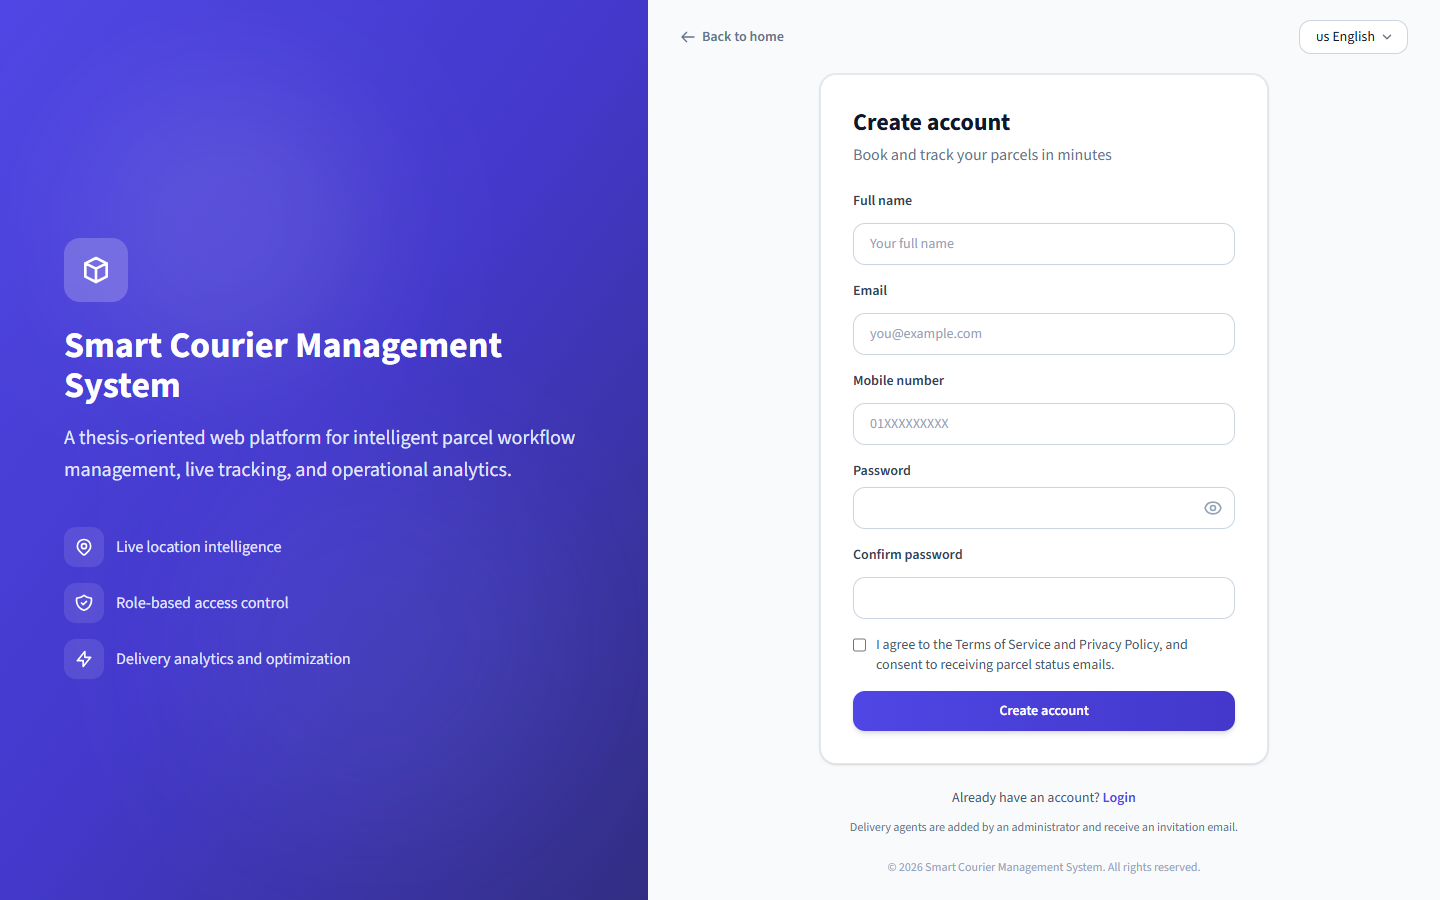
\includegraphics[width=0.85\textwidth]{figures/screenshots/register.png}
\caption{Customer registration page (running system)}
\label{fig:shot-register}
\end{figure}

\textbf{Login.} The login handler looks up the user with the hidden lockout fields. For unknown e-mails it still performs a bcrypt comparison against a dummy hash, so response time does not reveal whether an account exists. The lock is checked \emph{before} the password, so a correct guess during a lockout also fails. Five consecutive failures lock the account for 15 minutes. The account's active and verified states are revealed only after the password has been proven correct.

\textbf{Tokens and sessions.} A successful sign-in returns a JWT access token (HS256, issuer-checked, 15 minutes) containing the user id, role and \code{tokenVersion} (\code{tv}). It also sets a refresh cookie \code{scpms_rt}, a 384-bit random value, \code{HttpOnly}, \code{Secure} in production, \code{SameSite=Lax}, with path \code{/api/auth}. The frontend keeps the access token only in a JavaScript variable (\code{api.js}), never in \code{localStorage}. A timer refreshes the token one minute before expiry, and concurrent 401 responses share a single refresh request. Figure~\ref{fig:seq-session} shows the complete flow. When a refresh request arrives, the server handles the presented cookie as follows:
\begin{enumerate}
  \item It looks up the session by the hash of the cookie value. An unknown, expired or revoked session is refused (\code{NO_SESSION}).
  \item If the session was already rotated less than 30 seconds earlier, the request is treated as a harmless race between two browser tabs (\code{REFRESH_RACE}).
  \item If the session was rotated longer ago, the old cookie has been replayed, which indicates theft. Every session in the same rotation family is revoked (\code{TOKEN_REUSE}), so the legitimate user must also sign in again.
  \item Otherwise the session is marked as rotated, a new session with a fresh cookie is created in the same family, and a new access token is returned.
\end{enumerate}

\begin{figure}[htbp]
\centering
\resizebox{0.95\textwidth}{!}{% Sequence: sign-in, silent refresh with rotation and reuse detection
% (derived from auth.controller.js, session.service.js, frontend/src/api.js)
\begin{tikzpicture}[font=\scriptsize, >=Stealth]
\def\B{-12.2}
\seqhead{0}{b}{cCust}{Browser (React)}{\B}
\seqhead{6.0}{api}{cCore}{Express API}{\B}
\seqhead{11.0}{db}{cData}{Session collection}{\B}

% ---------------- sign in
\seqphase{-3.0}{12.2}{-0.75}{-3.85}{cCust}{1  SIGN IN}
\seqact{6.0}{-1.2}{-3.55}{cCore}
\seqmsg[cCust]{0}{5.91}{-1.35}{1}{POST /auth/login \{email, password, remember\}}
\seqnote{6.25}{-1.55}{lock check $\rightarrow$ bcrypt compare\\$\rightarrow$ active and verified}
\seqmsg[cData]{6.09}{11.0}{-2.65}{2}{store SHA-256(token), new family}
\seqret{5.91}{0}{-3.4}{access JWT (15 min, in memory)\\+ HttpOnly refresh cookie}

% ---------------- refresh
\seqphase{-3.0}{12.2}{-4.05}{-7.5}{cCore}{2  REFRESH}
\seqmsg[cCust]{0}{5.91}{-4.6}{3}{API requests with Authorization: Bearer}
\seqnote{0.3}{-4.95}{token near expiry, or 401 TOKEN\_EXPIRED}
\seqact{6.0}{-5.95}{-7.3}{cCore}
\seqmsg[cCust]{0}{5.91}{-6.1}{4}{POST /auth/refresh\\(cookie + X-Requested-With)}
\seqmsg[cData]{6.09}{11.0}{-6.6}{5}{mark old token rotated; store new hash}
\seqret{5.91}{0}{-7.15}{new access JWT + rotated cookie}

% ---------------- reuse detection
\seqphase{-3.0}{12.2}{-7.65}{-11.9}{cRed}{3  REUSE}
\pic at (-2.0,-8.05) {person=cRed};
\draw[cRed!60, line width=0.7pt, dash pattern=on 3pt off 2pt] (-2.0,-8.75) -- (-2.0,\B+0.3);
\seqact{6.0}{-8.25}{-11.45}{cRed}
\seqmsg[cRed]{-2.0}{5.91}{-8.4}{6}{attacker replays the old (already rotated) cookie}
\seqnote{6.25}{-8.6}{rotated more than 30 s ago\\$\Rightarrow$ reuse detected}
\seqmsg[cRed]{6.09}{11.0}{-9.65}{7}{revoke the whole token family}
\seqret[cRed]{5.91}{-2.0}{-10.3}{401 TOKEN\_REUSE}
\seqret[cRed]{5.91}{0}{-11.15}{legitimate session also ends: sign in again}
\end{tikzpicture}
}
\caption{Sequence diagram: sign-in, silent refresh with rotation, and reuse detection}
\label{fig:seq-session}
\end{figure}

The 30-second grace window handles a real case found during development: two browser tabs refreshing at the same moment present the same cookie, and the second request should not be treated as theft. The client retries once after a short delay when it receives \code{REFRESH_RACE}. Sessions last one day, or 30 days with ``Keep me signed in''. The two cookie-authenticated endpoints (\code{/auth/refresh} and \code{/auth/logout}) additionally require the header \cmd{X-Requested-With: XMLHttpRequest}, which a cross-site form cannot send.

\textbf{Password reset and revocation.} The forgot-password endpoint always returns the same message. When the account exists, it e-mails a single-use link whose token is stored hashed and expires after 30 minutes. Completing a reset increments \code{tokenVersion} and revokes all sessions. The same mechanism signs a user out everywhere when an administrator disables the account. \code{requireAuth} reloads the user on every request and rejects a token whose \code{tv} no longer matches.

\section{Authorisation}
\label{sec:impl-authz}

Authorisation is enforced on the server in two layers. The first layer is route guards: \code{requireAuth} verifies the token and loads the user, and \code{requireRoles(...)} admits only the listed roles. For example, booking is \code{requireRoles('customer')}, assignment and deletion are \code{requireRoles('admin')}, and location updates are \code{requireRoles('agent')}. The second layer is object-level checks in the controllers. \code{getParcel} returns a parcel only to its owner, its assigned agent or an administrator. \code{listParcels} adds a filter on \code{customer} or \code{agent} according to the role. \code{updateStatus} and \code{updateLocation} accept agents only for parcels assigned to them.

On the client, \code{ProtectedRoute}, \code{AdminRoute}, \code{DeliveryAgentRoute} and \code{CustomerRoute} redirect users away from pages for other roles. These guards improve usability but are not a security boundary, since the server repeats every check.

\section{Parcel Booking and Lifecycle}
\label{sec:impl-lifecycle}

\textbf{Booking.} Customers book from their dashboard (Figure~\ref{fig:shot-customer}). \code{createParcel} validates the addresses (1--300 characters), the enumerated fields, the COD amount (0--500{,}000, forced to 0 for prepaid parcels) and the notes ($\leq$500 characters). It then creates the parcel with an initial Pending history entry. The tracking code consists of ten characters drawn with \code{crypto.randomInt} from a 32-symbol alphabet that omits the easily confused characters 0, O, 1 and I. This gives $32^{10} = 2^{50}$ possible codes, which together with the rate limit on the public endpoint makes enumeration impractical. On the rare event of a duplicate code, creation is retried up to three times.

\begin{figure}[htbp]
\centering
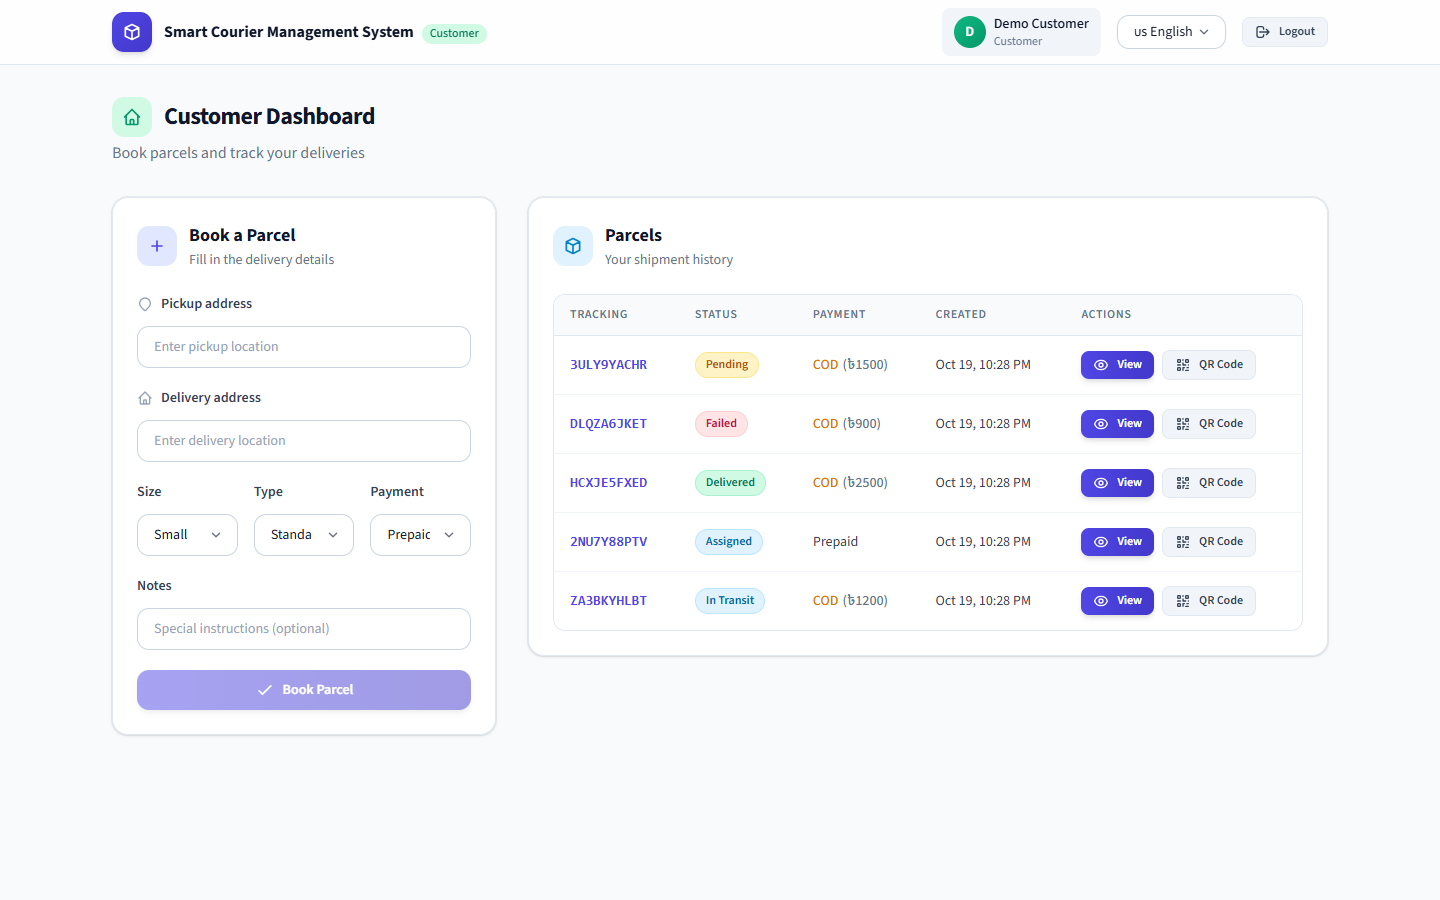
\includegraphics[width=0.9\textwidth]{figures/screenshots/customer-dashboard.png}
\caption{Customer dashboard with booking form and parcel list (running system, demonstration data)}
\label{fig:shot-customer}
\end{figure}

\textbf{Transitions.} All status changes go through one server-side rule, which encodes the state machine of Figure~\ref{fig:statemachine}. The rule applies its checks in a fixed order (Table~\ref{tab:transition-checks}). The first check that fails produces an explanatory error message, and the change is refused.

\begin{table}[htbp]
\centering
\caption{Order of checks applied to every requested status change}
\label{tab:transition-checks}
\small
\begin{tabularx}{\textwidth}{@{}p{0.6cm}LP{4.2cm}@{}}
\toprule
\textbf{No.} & \textbf{Check} & \textbf{Outcome} \\
\midrule
1 & The requested status equals the current status & Refused (``already in this state'') \\
2 & The parcel is Delivered or Failed & Refused for every role (final states are locked) \\
3 & The requester is an administrator & Allowed \\
4 & The parcel is not yet assigned to an agent (Pending) & Refused for agents \\
5 & The requested status is Failed & Allowed for the assigned agent \\
6 & The requested status lies before the current one, or is Pending or Assigned & Refused (agents only move forward) \\
7 & Any other forward move, including skipping states & Allowed \\
\bottomrule
\end{tabularx}
\end{table}

After a permitted change, the controller appends a history entry (status, time, actor and role) and saves the parcel. It then refreshes the agent's cached room list, pushes \code{parcel:update} to the watchers, and starts the status e-mail without waiting for it.

The agent's parcel page (Figure~\ref{fig:shot-agent-parcel}) shows the progress along the lifecycle, a status selector and controls for sending the current or a searched location.

\begin{figure}[htbp]
\centering
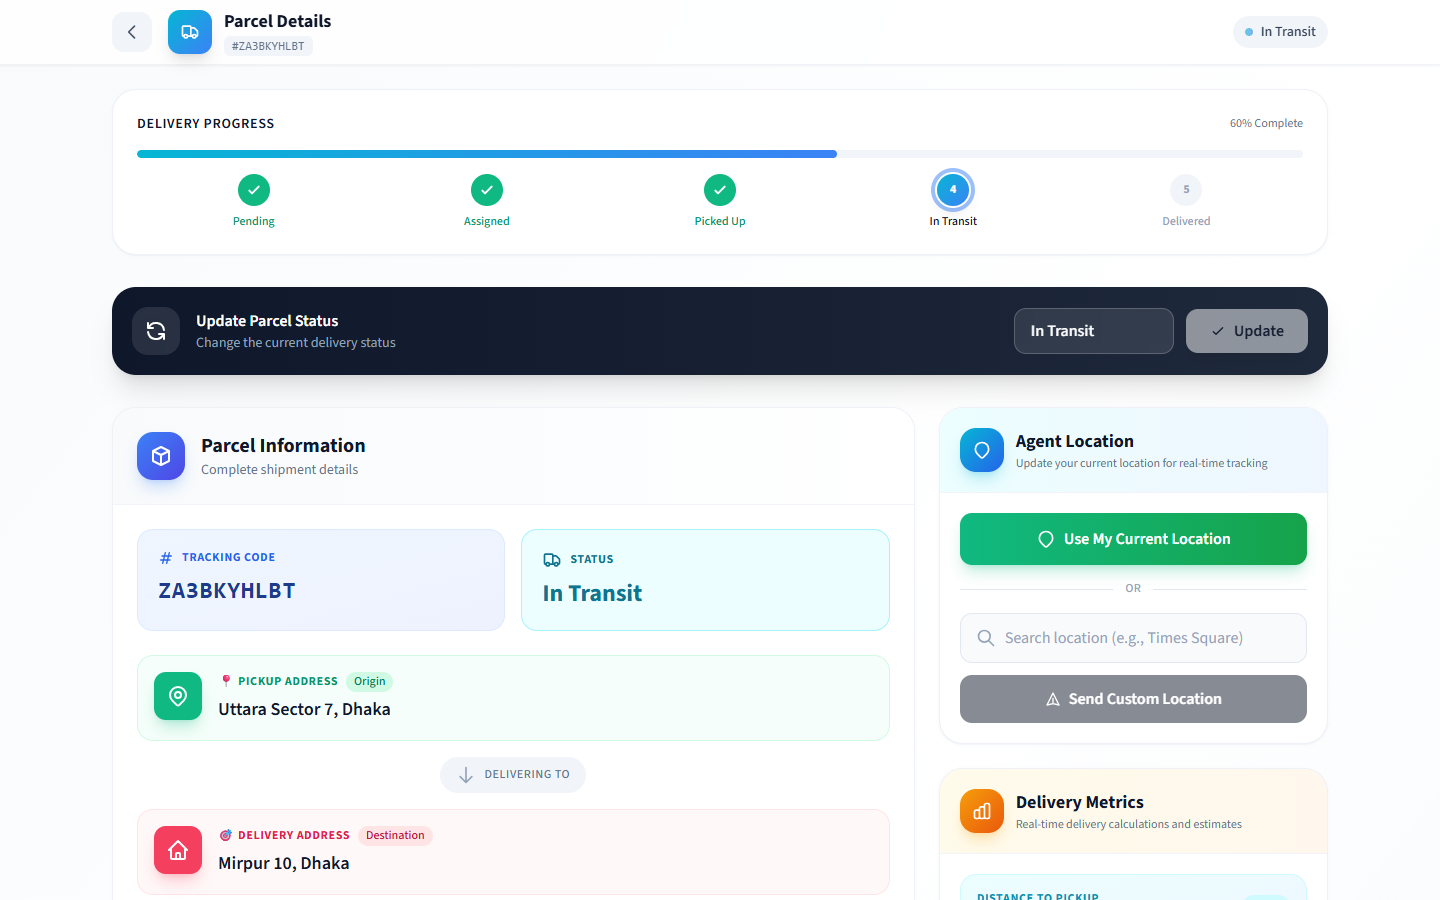
\includegraphics[width=0.9\textwidth]{figures/screenshots/agent-parcel-view.png}
\caption{Agent parcel page with lifecycle progress, status update and location controls (running system)}
\label{fig:shot-agent-parcel}
\end{figure}

\section{Real-Time Layer}
\label{sec:impl-realtime}

\code{services/socket.js} registers a Socket.IO middleware that reads \code{socket.handshake.auth.token}. If the token is valid and the user is active with a matching \code{tokenVersion}, it attaches \texttt{\{id, role\}} to the socket. Otherwise the socket stays anonymous. On connection, authenticated sockets join \code{user:<id>}, and administrators also join \code{role:admin}. The client reads the in-memory token at every (re)connection and reconnects after sign-in and sign-out, so the server always re-evaluates identity.

\code{services/realtime.js} provides \code{emitToParcel}, which sends to \code{role:admin}, \code{parcel:<id>}, the owning customer's room and the assigned agent's room, and \code{emitToAdmins}. Controllers emit only through these helpers. When an agent's browser sends a position, the server processes it in four steps:
\begin{enumerate}
  \item It discards the message unless the socket belongs to a signed-in agent and the agent identifier in the message is that agent's own identifier. This prevents anyone from spoofing another agent's position.
  \item It discards coordinates outside the valid latitude and longitude ranges.
  \item It stores the position in memory as the agent's last known location, with a timestamp.
  \item It forwards the position only to the administrators' room and to the rooms of the agent's active parcels (their watchers and owning customers).
\end{enumerate}
To avoid one database query per GPS update, the list of rooms for an agent's active parcels is cached for 15 seconds and refreshed whenever an assignment or status changes.

Administrators follow agents on the tracking page (Figure~\ref{fig:shot-tracking}). Selecting an agent loads that agent's parcels and sends \code{request:agent:location}. The server replies with the last known position and asks that agent's client, and only that client, for a fresh one.

\begin{figure}[htbp]
\centering
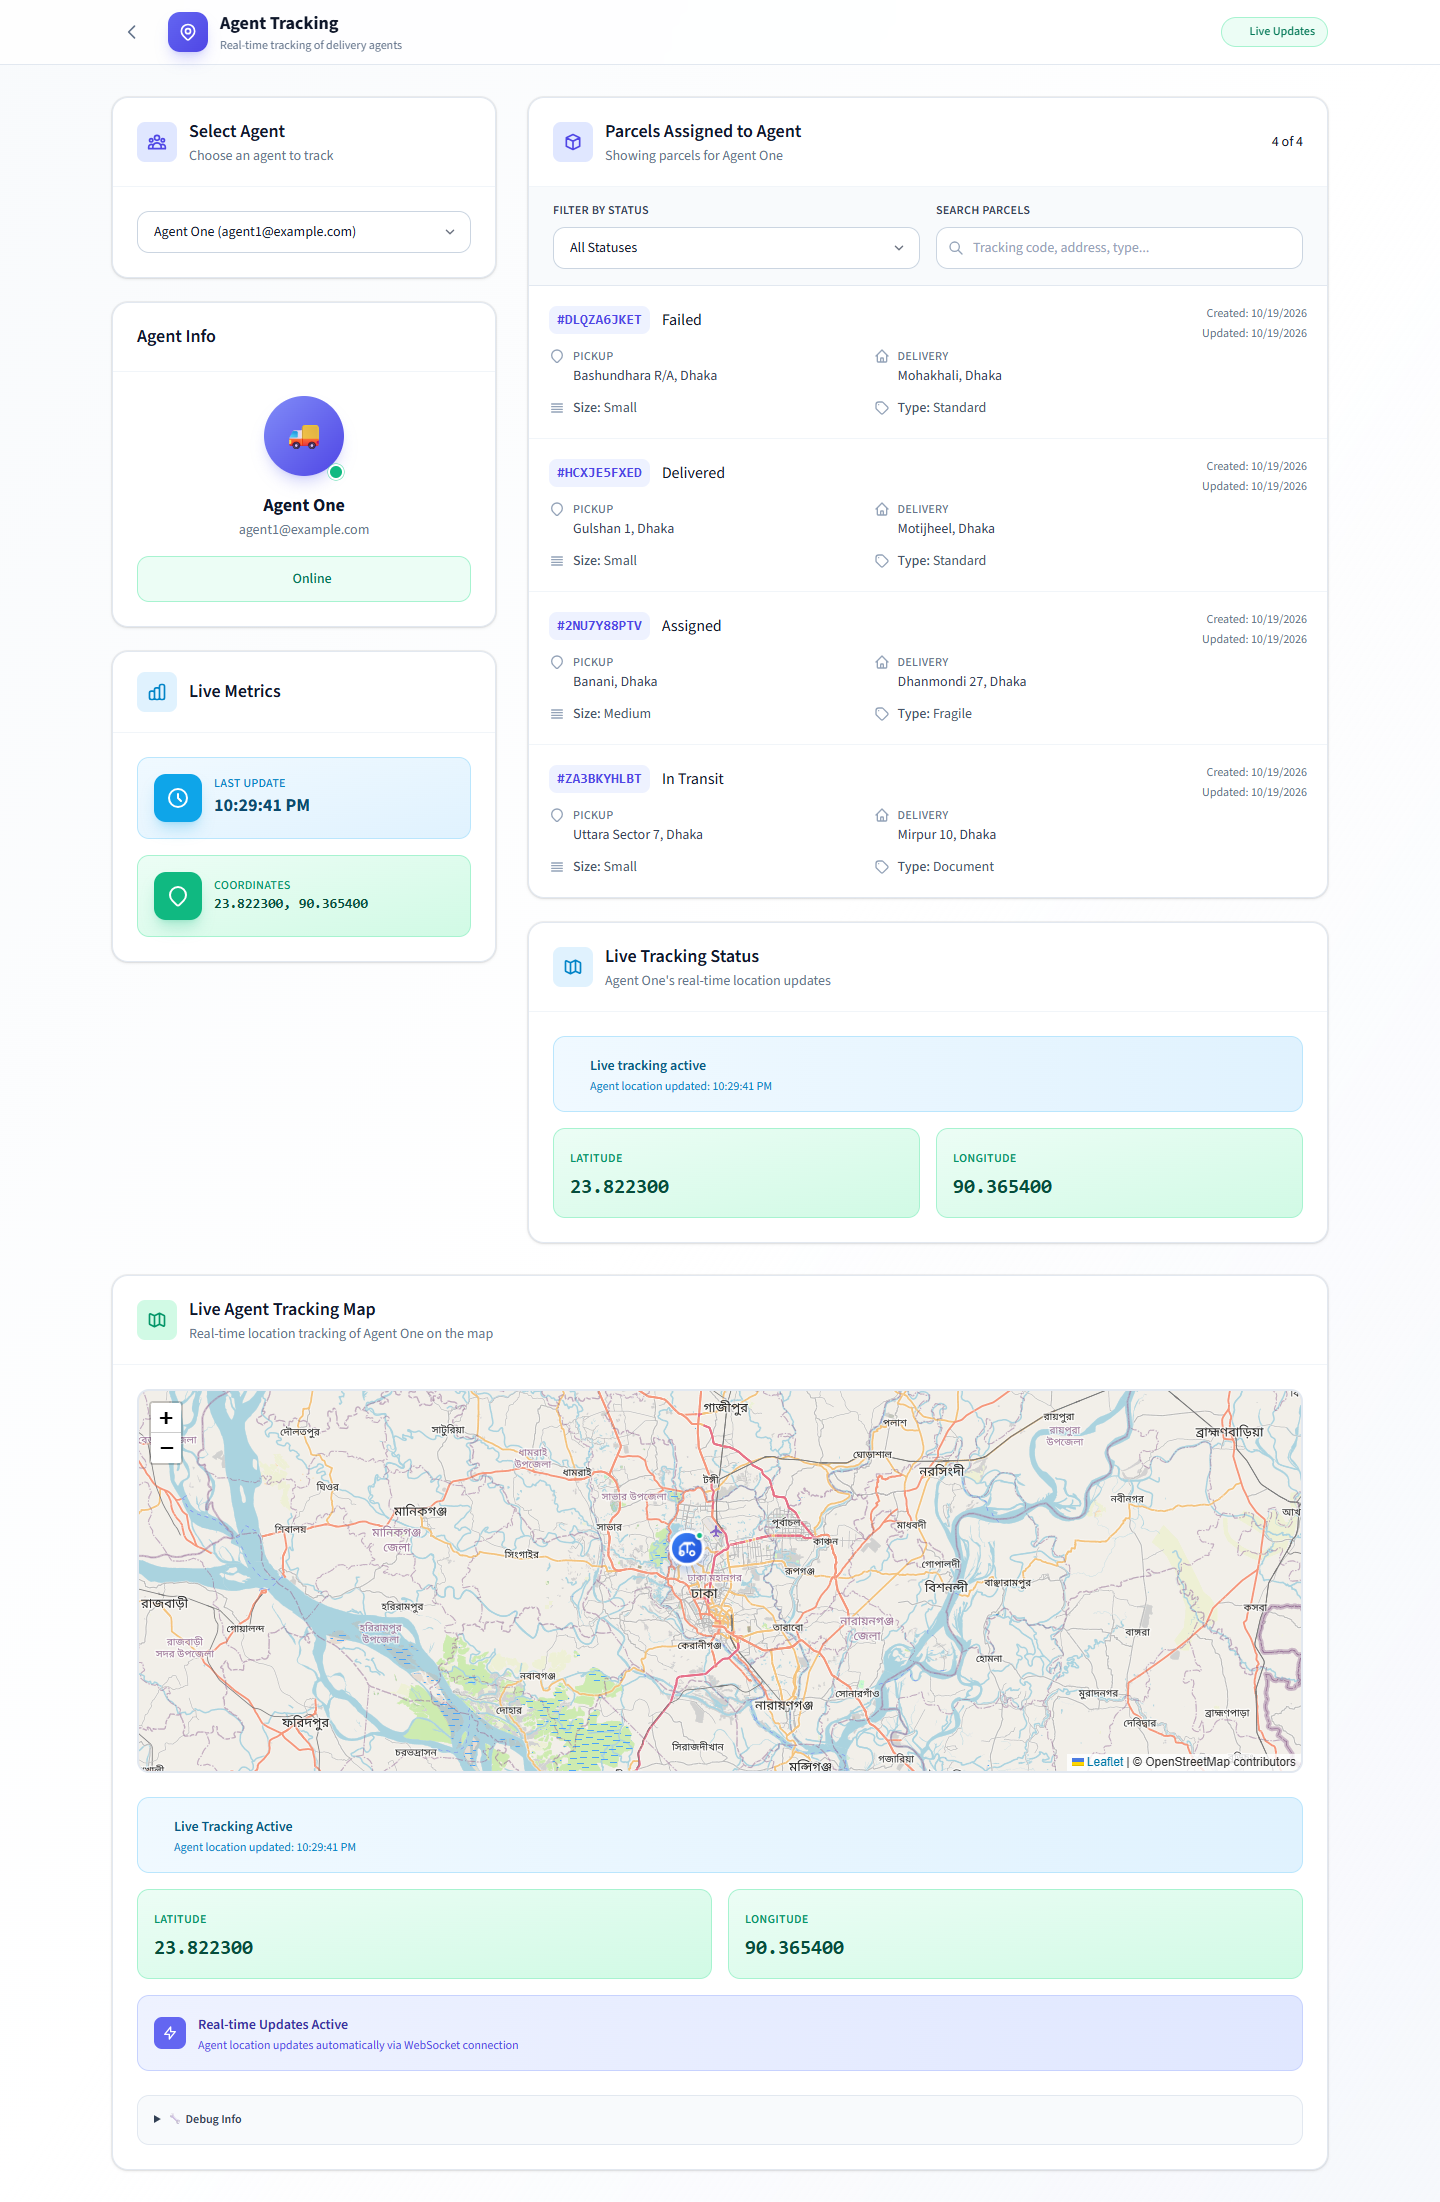
\includegraphics[width=0.78\textwidth]{figures/screenshots/admin-agent-tracking.png}
\caption{Administrator agent-tracking page receiving a live position from a connected agent (running system; position simulated)}
\label{fig:shot-tracking}
\end{figure}

\section{Location, Maps and Estimated Arrival}
\label{sec:impl-maps}

\textbf{Capturing location.} The agent dashboard calls \code{navigator.geolocation.watchPosition} with high accuracy. Each new position is throttled and skipped if unchanged, emitted on the socket, and posted through REST to every parcel that is In Transit. The agent's parcel page additionally sends the current position every 20 seconds, and allows a typed address to be geocoded and sent instead (for example when GPS is unavailable). The server accepts REST location updates only from the assigned agent and only for active parcels.

\textbf{Geocoding.} Addresses are free text. The backend route \code{/api/geocode/search} appends ``Bangladesh'', queries Photon biased towards Dhaka, and falls back to Nominatim with \code{countrycodes=bd} and an identifying \code{User-Agent} header. The route is rate-limited and caps the number of results at five, so it cannot be used for bulk lookups.

\textbf{Maps and routes.} Leaflet renders OSM tiles. leaflet-routing-machine requests a road route between the geocoded pickup and delivery points from the public OSRM demonstration server and draws it (Figures~\ref{fig:shot-public} and~\ref{fig:shot-customer-detail}). One page (\code{PublicTrack.jsx}, at \code{/track/:code}) uses the Google Maps JavaScript API instead. Its API key is not present in the repository's production environment file, so that page shows a map error unless the key is configured on the hosting platform. The Leaflet page \code{/track-parcel}, linked from status e-mails, does not depend on Google.

\begin{figure}[htbp]
\centering
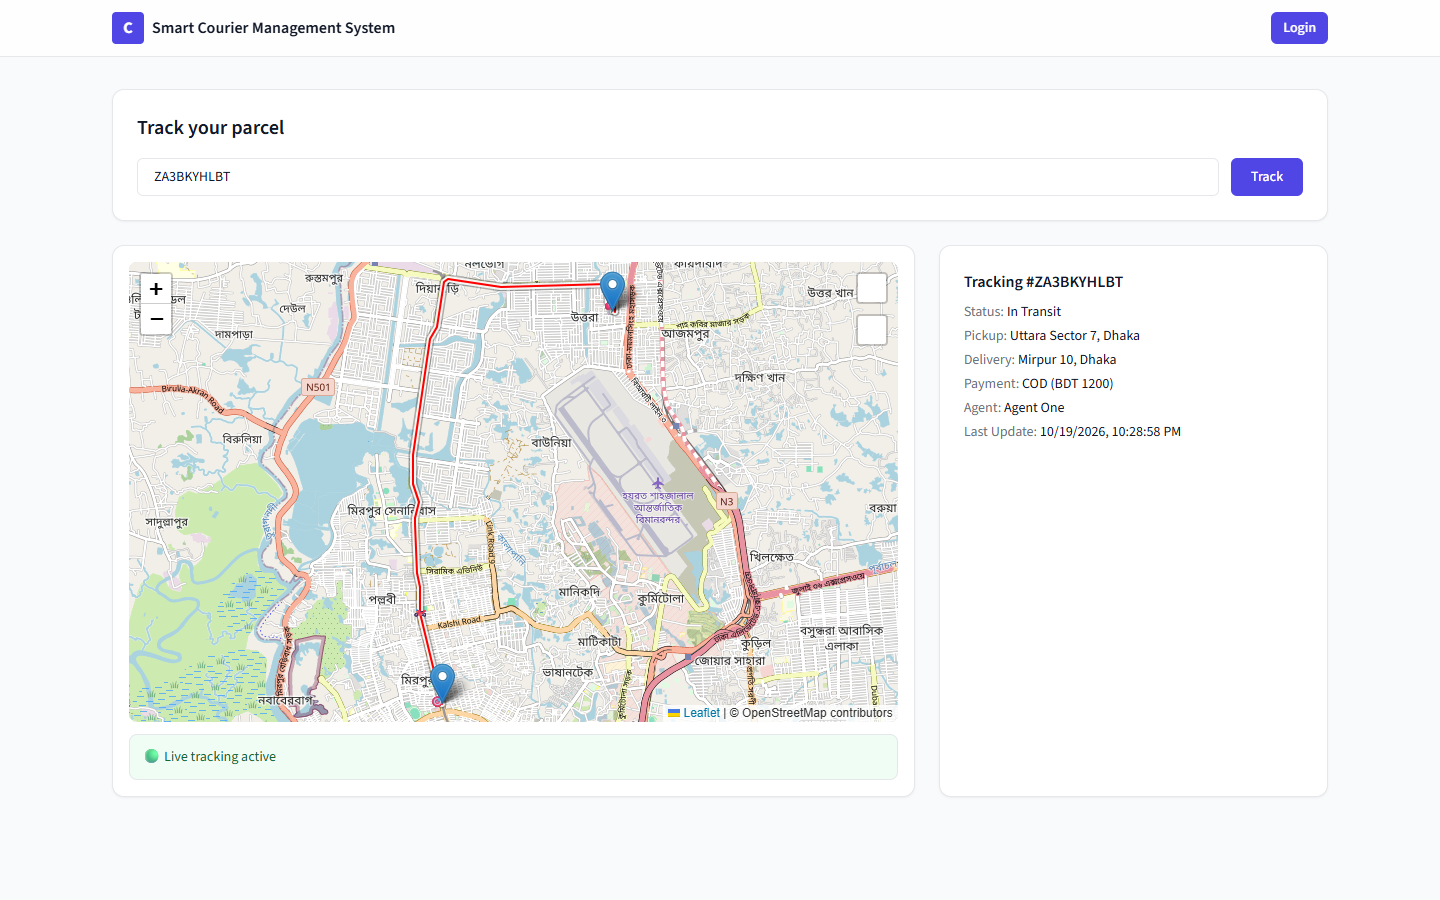
\includegraphics[width=0.9\textwidth]{figures/screenshots/public-tracking.png}
\caption{Public tracking by code with OSM map and OSRM route; no customer data is shown (running system)}
\label{fig:shot-public}
\end{figure}

\textbf{Estimated arrival.} The customer parcel page computes the straight-line (haversine) distance from the agent's latest position to the geocoded delivery point. It divides this distance by the agent's observed speed, or by 25\,km/h when no speed is known, to display an ETA (Figure~\ref{fig:shot-customer-detail}). This is a simple heuristic, not a road-network or traffic-aware prediction, and it is presented as such in this report. The server stores \code{etaMinutes} only when a client supplies it.

\begin{figure}[htbp]
\centering
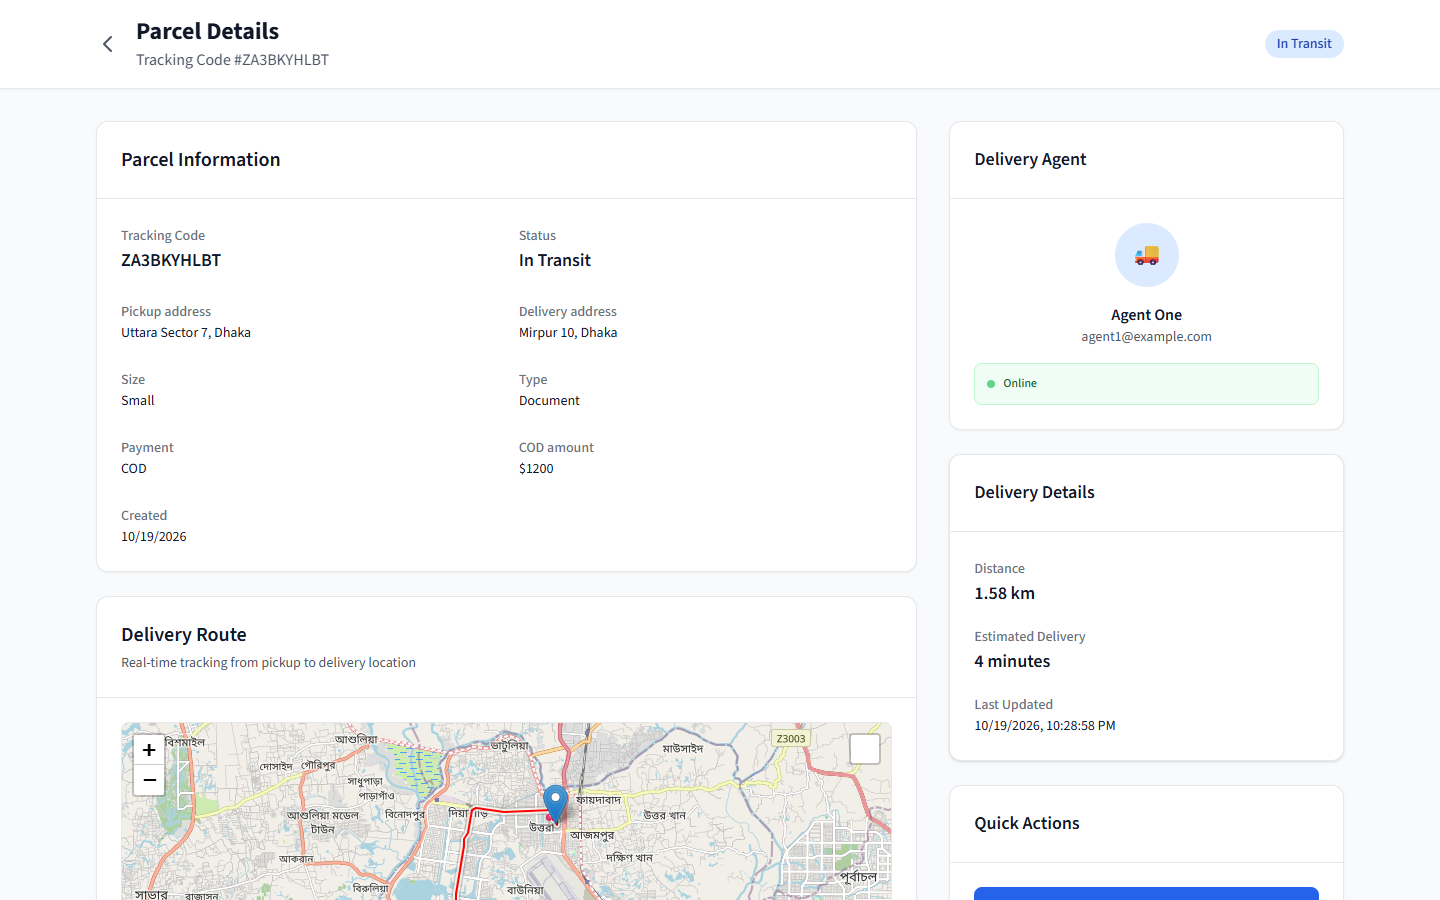
\includegraphics[width=0.9\textwidth]{figures/screenshots/customer-parcel-detail.png}
\caption{Customer parcel page with agent card, distance and heuristic ETA (running system). The COD amount is shown with a ``\$'' sign, a currency-symbol defect recorded in Chapter~\ref{chap:results}}
\label{fig:shot-customer-detail}
\end{figure}

\section{QR-Assisted Pickup}
\label{sec:impl-qr}

For each parcel the customer can open a QR page (Figure~\ref{fig:shot-qr}). The page encodes the URL \code{<origin>/customer/parcel/qr/<parcelId>} with the \code{qrcode} library at error-correction level~M, and offers a print button. The agent opens ``Pickup Scan'' from the dashboard. The scanner uses the browser's native \code{BarcodeDetector} when available, sampling the rear camera every 250\,ms, and otherwise falls back to ZXing. It extracts the parcel id from the scanned URL and opens the confirmation page (Figure~\ref{fig:shot-pickup}). Confirming sends \texttt{\{status: "Picked Up"\}}. If the camera cannot be used, the agent can paste the link or the parcel id.

\begin{figure}[htbp]
\centering
\begin{subfigure}[t]{0.49\textwidth}
  \centering
  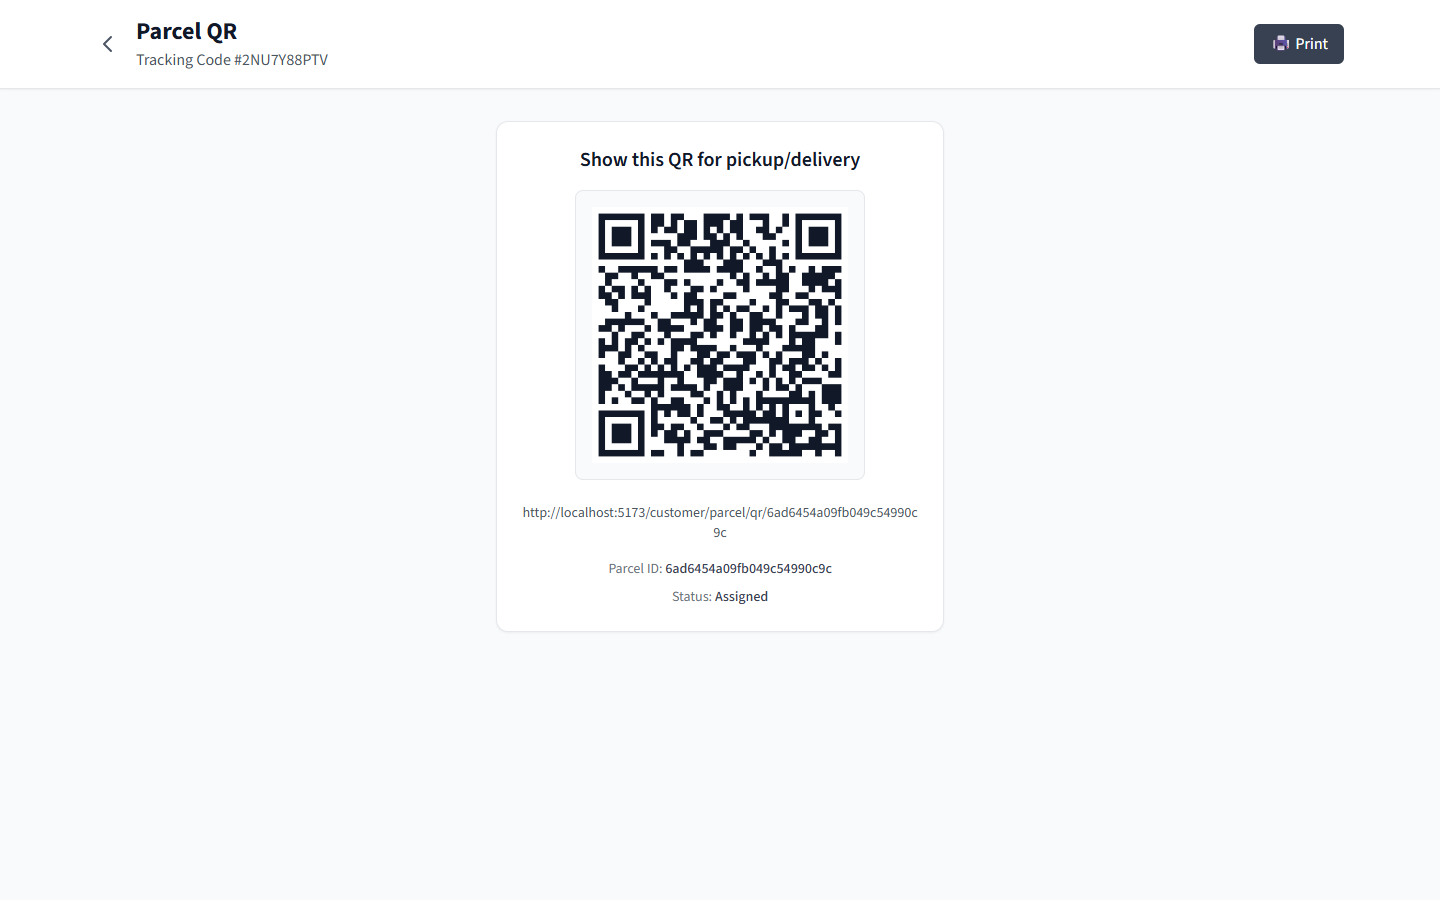
\includegraphics[width=\textwidth]{figures/screenshots/customer-qr.png}
  \caption{Customer's parcel QR page}
  \label{fig:shot-qr}
\end{subfigure}\hfill
\begin{subfigure}[t]{0.49\textwidth}
  \centering
  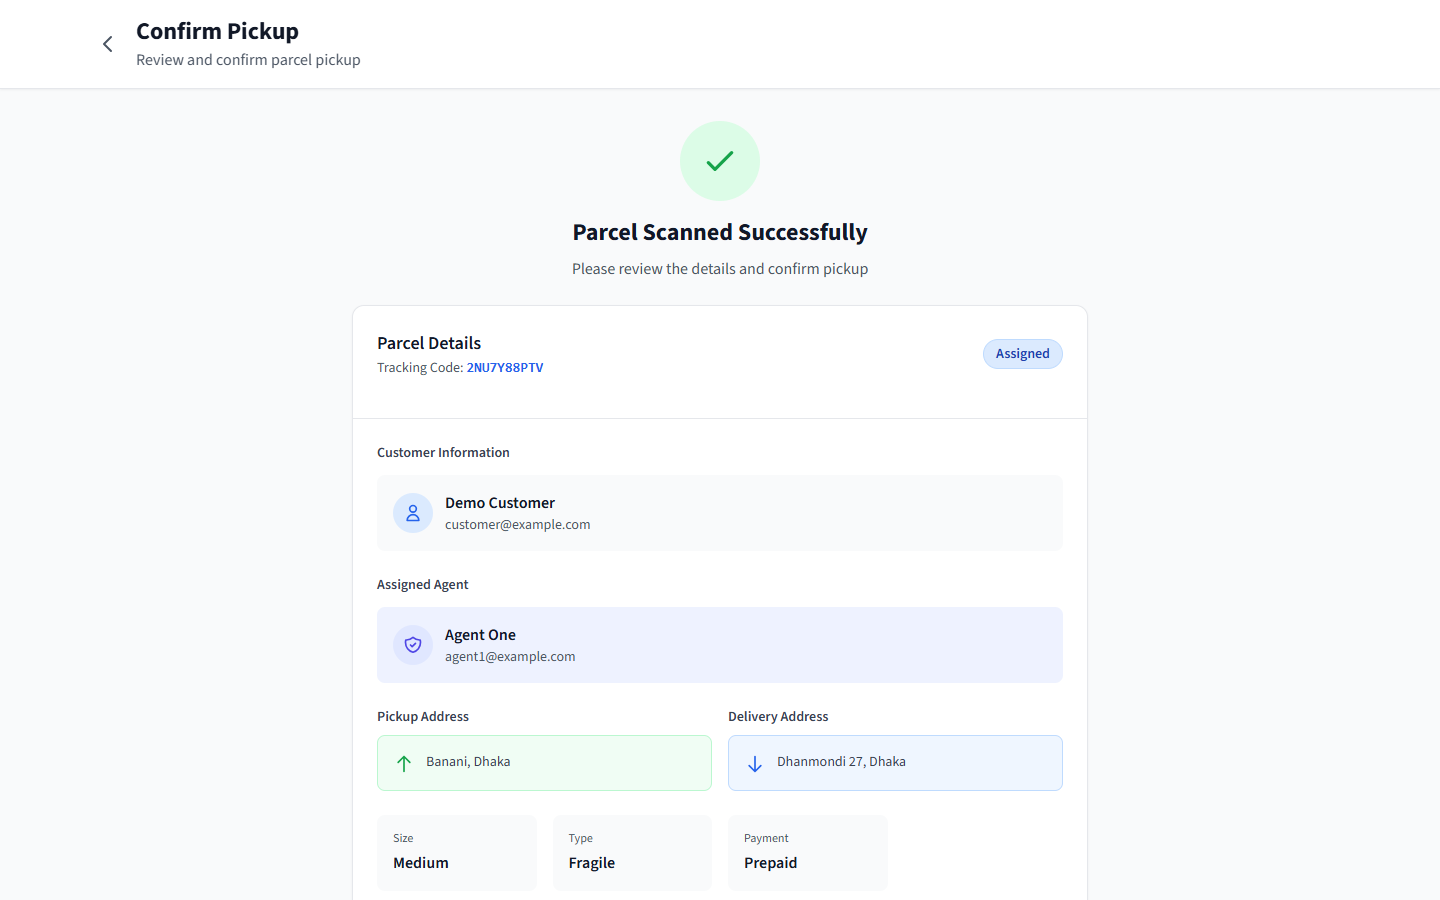
\includegraphics[width=\textwidth]{figures/screenshots/agent-pickup-confirm.png}
  \caption{Agent's pickup confirmation page}
  \label{fig:shot-pickup}
\end{subfigure}
\caption{QR-assisted pickup (running system). The confirmation page is normally reached by scanning; for the screenshot it was opened directly by URL}
\label{fig:shot-qrflow}
\end{figure}

It is important to state precisely what the QR step achieves. It \emph{identifies} the parcel quickly and reduces the chance that an agent confirms the wrong parcel. It is \emph{not} a cryptographic proof of handover. The QR content is the parcel's database identifier, and the manual fallback accepts the same identifier. The security guarantee comes from the server, which accepts the Picked Up transition only from the agent assigned to that parcel. The QR page's heading mentions ``pickup/delivery'', but scanning is implemented only for pickup. Earlier project documents that describe QR verification at delivery, or OTP delivery confirmation, describe features that are not present: the OTP interface was removed during the security review because it had no backend.

\section{Notifications}
\label{sec:impl-notify}

\code{utils/mailer.js} builds HTML e-mails with a shared layout and escapes all user-supplied text to prevent HTML injection. Four message types exist: the verification code, the password-reset link, the agent invitation (72-hour link) and the status-change notification. The status notification links to the public tracking page. It is sent asynchronously after the database update, and failures are only logged, so an unavailable SMTP server cannot delay or fail a status change. In production, an unconfigured mailer makes the verification, reset and invitation operations return 503. If an invitation cannot be e-mailed, the administrator is shown the link to share by another channel.

\section{Analytics, Export and User Management}
\label{sec:impl-analytics}

The administrator dashboard (Figure~\ref{fig:shot-admin}) shows three indicators computed by \code{dashboardMetrics}: bookings created since local midnight, the number of parcels in the Failed state, and the sum of COD amounts of delivered COD parcels (a MongoDB aggregation). The indicators refresh when \code{parcel:created} or \code{parcel:update} events arrive. The bookings table supports text search by tracking code or status and per-row assignment, and the assignment control locks once a parcel is past Assigned. The CSV export streams one row per parcel (tracking code, status, payment type, COD amount, creation time) with proper quoting. The PDF export writes the same fields as a simple list with PDFKit. The users panel lists all accounts with their state (active, unverified or invitation pending, disabled) and lets the administrator add agents, resend invitations and disable or re-enable accounts.

\begin{figure}[htbp]
\centering
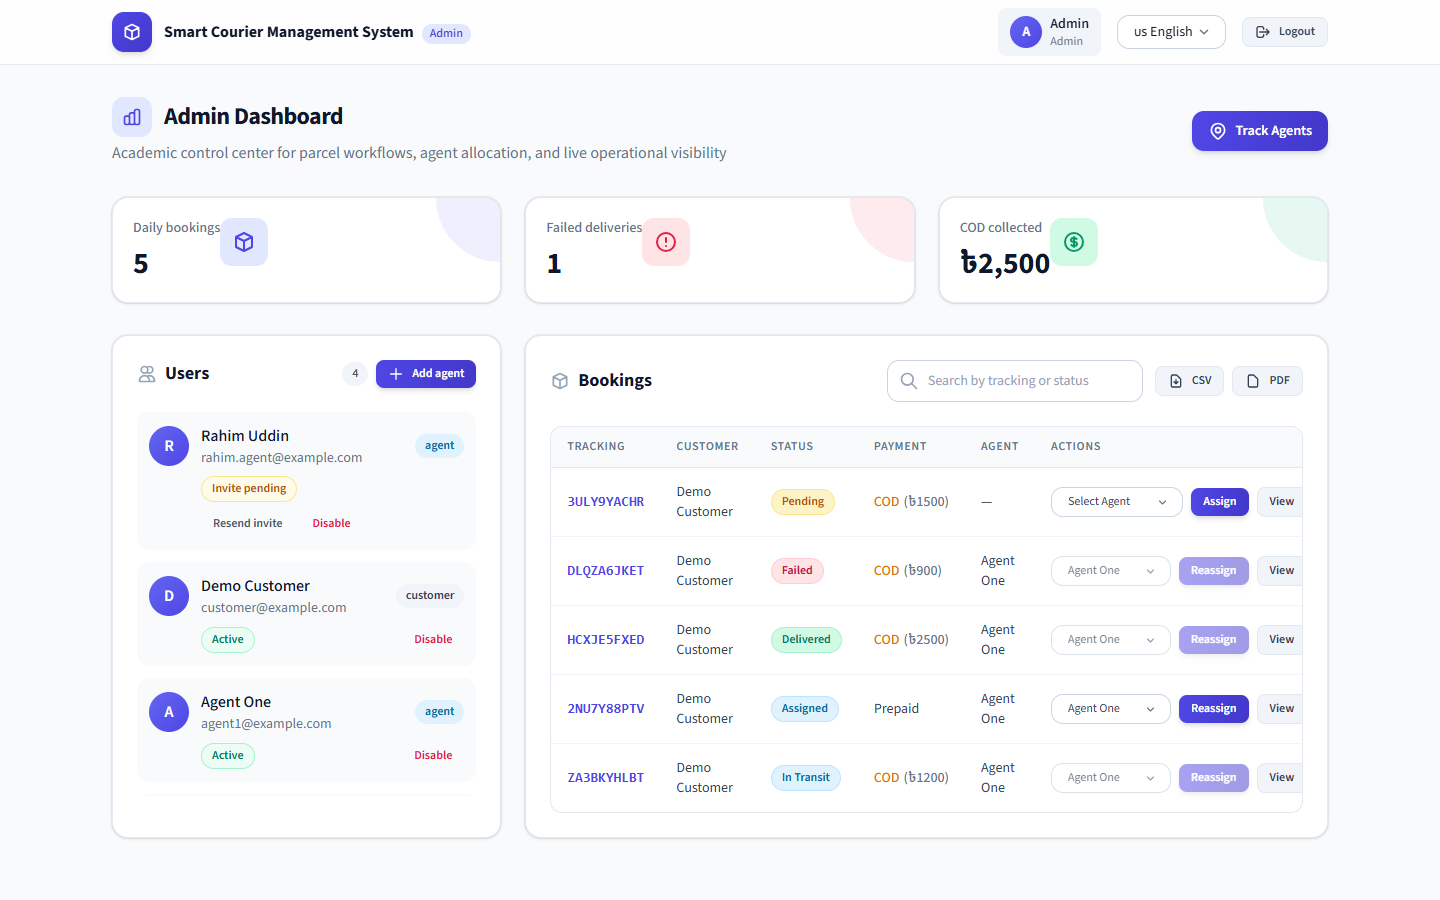
\includegraphics[width=0.95\textwidth]{figures/screenshots/admin-dashboard.png}
\caption{Administrator dashboard: indicators, user management, bookings with assignment and CSV/PDF export (running system, demonstration data)}
\label{fig:shot-admin}
\end{figure}

The analytics are deliberately basic. The system does not compute success rates over time, revenue trends, monthly reports, heat maps or delay risk, although some early documents listed them. They remain future work.

\section{Frontend Implementation and Internationalisation}
\label{sec:impl-frontend}

The frontend is a React single-page application. \code{App.jsx} defines public routes (landing, tracking, login, registration, verification, password reset), guest-only routes and role-guarded route groups. \code{AuthContext} restores the session on page load by calling the refresh endpoint (the access token is not persisted), schedules the next refresh and reconnects the shared socket when identity changes. \code{api.js} attaches the bearer token, retries once after a successful refresh on token errors, and converts server errors into an \code{ApiError} carrying the machine-readable code (for example \code{EMAIL_NOT_VERIFIED}). The UI uses these codes to show helpful messages.

\begin{figure}[htbp]
\centering
\begin{subfigure}[t]{0.49\textwidth}
  \centering
  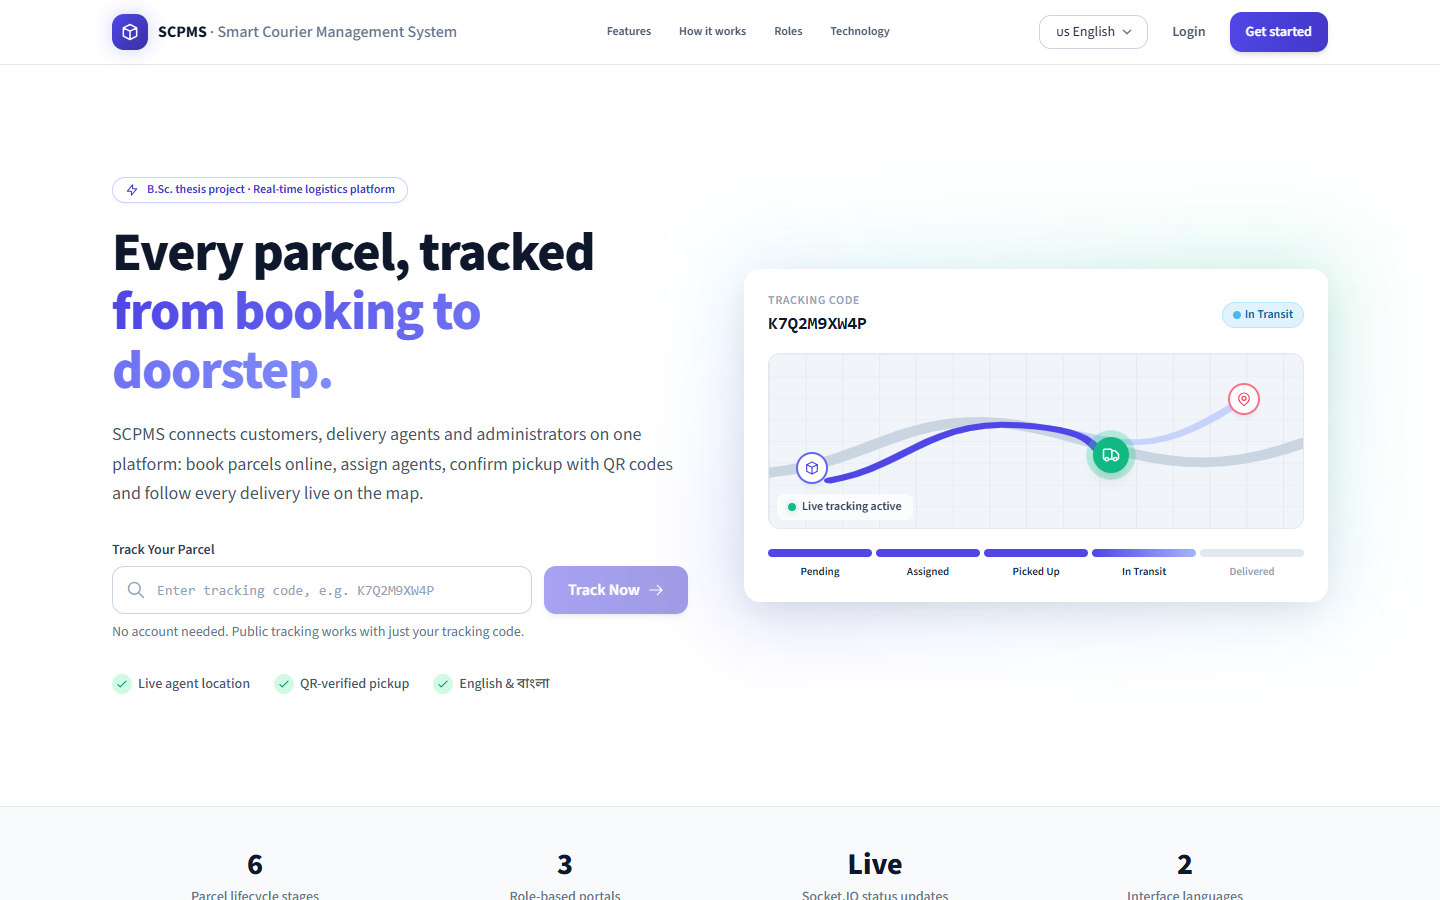
\includegraphics[width=\textwidth]{figures/screenshots/landing.png}
  \caption{English}
\end{subfigure}\hfill
\begin{subfigure}[t]{0.49\textwidth}
  \centering
  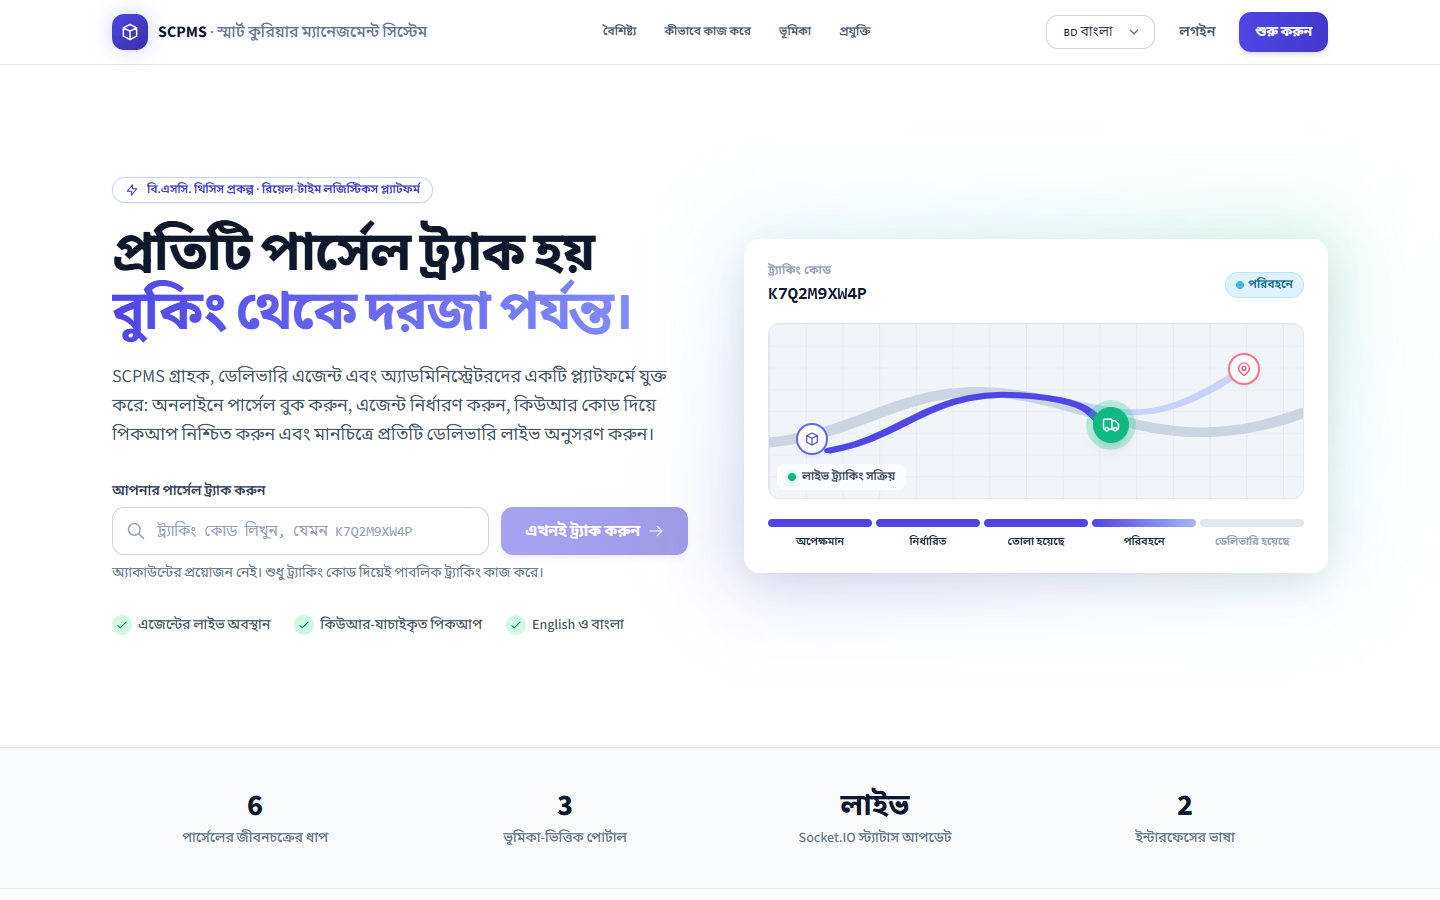
\includegraphics[width=\textwidth]{figures/screenshots/landing-bn.png}
  \caption{Bangla}
\end{subfigure}
\caption{Landing page with public tracking entry in both interface languages (running system)}
\label{fig:shot-landing}
\end{figure}

\code{LanguageContext} stores the chosen language in \code{localStorage}, and each component reads its strings from \code{translations/en.js} or \code{bn.js}, which hold about 320 entries each. Figure~\ref{fig:shot-landing} shows the landing page in both languages. The agent dashboard (Figure~\ref{fig:shot-agent}) summarises the agent's parcels, shows the socket connection state and a live OSM map of the agent's own position, and links to the pickup scanner.

\begin{figure}[htbp]
\centering
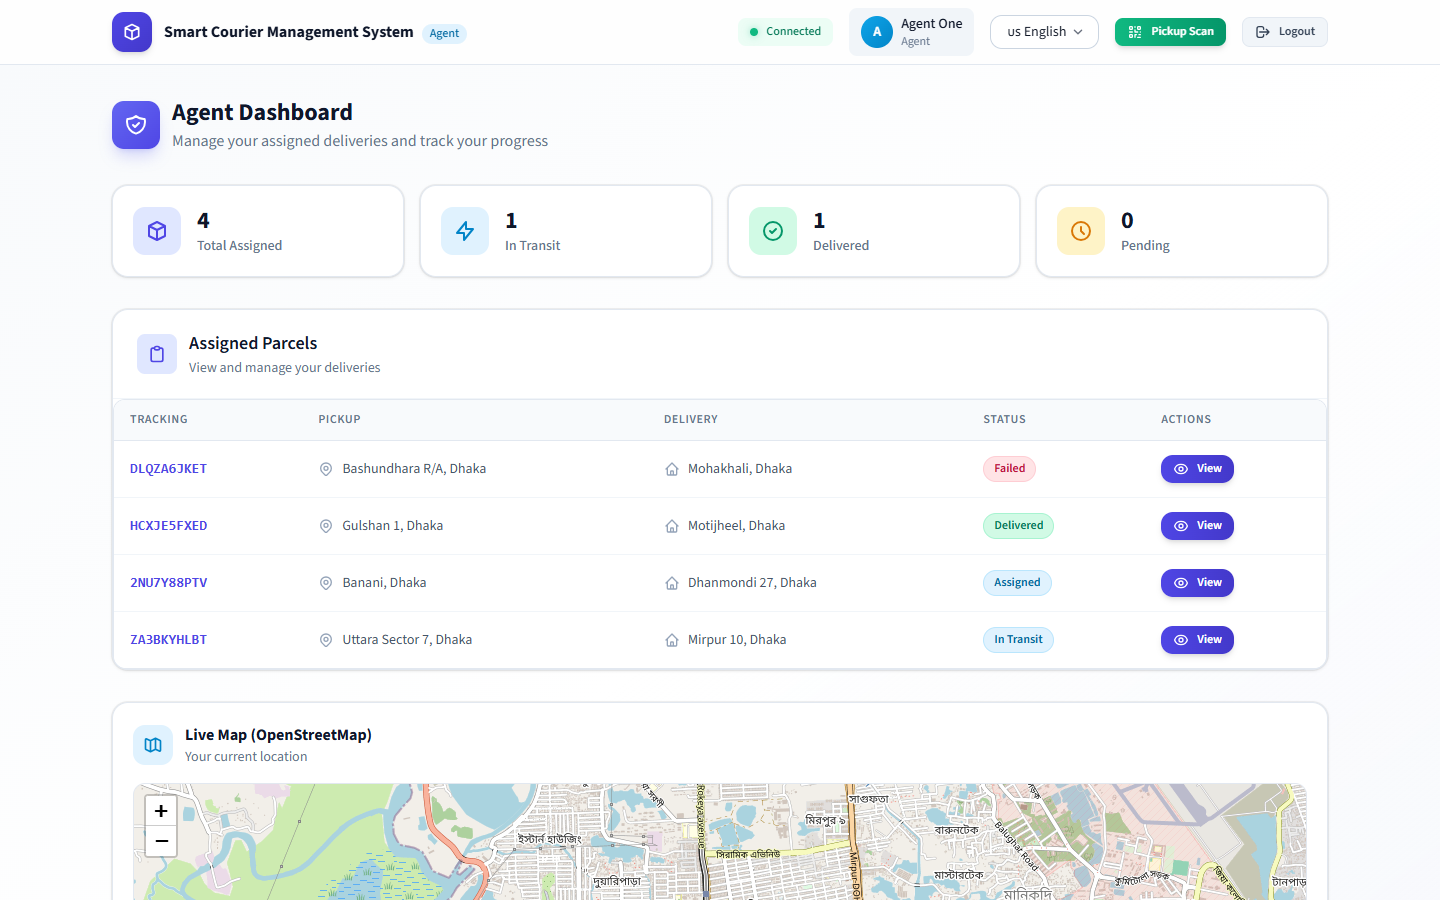
\includegraphics[width=0.9\textwidth]{figures/screenshots/agent-dashboard.png}
\caption{Delivery-agent dashboard (running system, demonstration data)}
\label{fig:shot-agent}
\end{figure}

\section{Validation, Error Handling and Hardening}
\label{sec:impl-hardening}

Input is validated at three levels. First, \code{middleware/sanitize.js} recursively removes every key that begins with \code{$} or contains \code{.} from the body, query string and route parameters, so values such as \texttt{\{"\$ne": null\}} can never reach MongoDB as operators \cite{ron2016nosql}. Second, controllers check types and ranges explicitly: identifiers with \code{isObjectId}, coordinates with \code{isValidLatLng}, strings with length limits, and enumerations against the shared constants. Third, Mongoose schema constraints act as a final safeguard. Mongoose's \code{strictQuery} option discards unknown query fields.

Rate limits are applied per endpoint: login (20 per 15 minutes), registration (10 per hour), code verification and password reset (20 per 15 minutes), e-mail-sending endpoints (5 per 15 minutes), refresh (120), public tracking (120) and geocoding (300 per 15 minutes), on top of the global limit. The number of trusted proxy hops is configurable (\code{TRUST_PROXY_HOPS}), so that the limiter sees real client addresses behind the hosting proxies. The frontend hosting configuration adds \code{X-Frame-Options}, \code{X-Content-Type-Options}, \code{Referrer-Policy}, HSTS and a \code{Permissions-Policy} that allows camera and geolocation only for the site itself.

\section{Deployment and Execution}
\label{sec:impl-deploy}

Figure~\ref{fig:deployment} shows the deployment that the repository is configured for. \code{backend/render.yaml} defines a Render web service with a \code{/health} check, \code{NODE_ENV=production}, two trusted proxy hops, a generated \code{JWT_SECRET}, and placeholders for the database URI, allowed origin, application URL and SMTP credentials. \code{frontend/vercel.json} and \code{netlify.toml} serve the built SPA, rewrite \code{/api/*} to the Render service and set security headers. \code{frontend/.env.production} sets \code{VITE_API_BASE=/api} and the socket URL. Whether this deployment is currently running was not verified as part of this work.

\begin{figure}[htbp]
\centering
\resizebox{\textwidth}{!}{% Deployment view (derived from backend/render.yaml, frontend/vercel.json, netlify.toml,
% frontend/.env.production). Whether the deployment is currently live was not verified.
\begin{tikzpicture}[font=\scriptsize, >=Stealth,
  box/.style={card=#1, minimum width=3.8cm, minimum height=1.9cm, align=center, text width=3.5cm},
  svc/.style={card=#1, minimum width=2.9cm, minimum height=1.5cm, align=center, text width=2.6cm}]

% ---------- zones
\node[panel=cCust, minimum width=4.6cm, minimum height=6.4cm] at (0,-1.15) {};
\node[tag=cCust] at (0,1.75) {CLIENT DEVICES};
\node[panel=cExt, minimum width=4.6cm, minimum height=3.1cm] at (5.8,0.5) {};
\node[tag=cExt] at (5.8,1.75) {STATIC HOSTING / EDGE};
\node[panel=cCore, minimum width=4.6cm, minimum height=3.1cm] at (11.6,0.5) {};
\node[tag=cCore] at (11.6,1.75) {APPLICATION TIER};
\node[panel=cData, minimum width=10.4cm, minimum height=2.6cm] at (8.7,-3.05) {};
\node[tag=cData, anchor=west] at (3.65,-4.35) {DATA AND THIRD-PARTY SERVICES};

% ---------- main nodes (icons sit in the reserved top area of each card)
\node[box=cCust] (browser) at (0,0.25) {\iconspace[8mm]\textbf{Browser}\\desktop or phone};
\pic at (-0.5,0.78) {browser=cCust}; \pic at (0.6,0.78) {phone=cCust};
\node[box=cExt] (cdn) at (5.8,0.25) {\iconspace[8mm]\textbf{Vercel / Netlify}\\SPA files, \code{/api/*} rewrite,\\security headers};
\node[cloud, cloud puffs=10, aspect=2, draw=cExt, fill=cExt!20, line width=0.8pt, minimum width=1.2cm, minimum height=0.65cm] at (5.8,0.85) {};
\node[box=cCore] (render) at (11.6,0.25) {\iconspace[8mm]\textbf{Render web service}\\Express + Socket.IO,\\health check \code{/health}};
\pic at (11.6,0.82) {server=cCore};

\node[svc=cData] (db) at (5.6,-3.25) {\iconspace[7mm]\textbf{MongoDB}\\\code{MONGODB_URI}};
\pic at (5.6,-2.88) {db=cData};
\node[svc=cExt] (smtp) at (8.7,-3.25) {\iconspace[7mm]\textbf{SMTP}\\Gmail (app password)};
\pic at (8.7,-2.86) {mail=cExt};
\node[svc=cExt] (geo) at (11.8,-3.25) {\iconspace[7mm]\textbf{Geocoding}\\Photon / Nominatim};
\pic at (11.8,-2.82) {pin=cRed};
\node[box=cExt, minimum height=1.6cm] (maps) at (0,-3.25) {\iconspace[7mm]\textbf{Map services}\\OSM tiles, OSRM demo, Google Maps JS};
\pic at (0,-2.82) {mapicon=cExt};

% ---------- connections
\draw[flow=cCust] (browser.east) -- node[elabel, above=2pt]{HTTPS: pages\\and \code{/api}} (cdn.west);
\draw[flow=cExt] (cdn.east) -- node[elabel, above=2pt]{proxied\\\code{/api}} (render.west);
\draw[rtflow] ($(browser.north east)+(-0.5,0.25)$) -- ++(0,1.25) -| node[pos=0.25, above, font=\scriptsize\bfseries, text=cSock]{WebSocket connection directly to the backend (\code{VITE_SOCKET_URL})} ($(render.north east)+(-0.25,0.25)$);
\draw[bflow=cData] ($(render.south)+(-1.2,0)$) -- (db.north east);
\draw[flow=cExt] ($(render.south)+(-0.3,0)$) -- (smtp.north);
\draw[bflow=cExt] ($(render.south)+(0.3,0)$) -- (geo.north);
\draw[bflow=cExt] (browser.south) -- (maps.north);

\node[font=\tiny, text=cExt, anchor=north west] at (-2.3,-4.75) {Configuration as defined in the project files; whether this deployment is currently live was not verified.};
\end{tikzpicture}
}
\caption{Deployment view as configured in the repository}
\label{fig:deployment}
\end{figure}

For local execution, the dependencies of both packages are installed from the repository root. A seed script creates the first administrator and agent; in production, their passwords must be supplied through environment variables. A single development script then starts the API on port 5000 and the web client on port 5173.

\section{Implementation Challenges}
\label{sec:challenges}

\begin{itemize}
  \item \textbf{Securing real-time channels.} The first version trusted the \code{agentId} sent by any socket and broadcast all agent positions to every client, so locations could be spoofed and leaked. Authenticating sockets with the access token and scoping every event to rooms solved both problems. It required the room cache to keep database load low during continuous GPS updates.
  \item \textbf{Cookies across hosting providers.} With the frontend and API on different domains, browsers that block third-party cookies dropped the refresh cookie. Routing \code{/api} through the frontend host made the cookie first-party.
  \item \textbf{Configuration loaded too late.} Some modules read \code{process.env} when imported, before \code{.env} had been loaded, so local SMTP and JWT settings were silently ignored. Loading \code{dotenv} as the first import fixed this.
  \item \textbf{Concurrent refreshes.} Rotating refresh tokens broke sessions when two tabs refreshed together. The 30-second grace window and a single client retry handle this race without weakening reuse detection.
  \item \textbf{Free map services.} Geocoding of informal Bangladeshi addresses is sometimes imprecise, and public routing and geocoding services impose rate limits. A backend proxy with Bangladesh bias and a Photon-to-Nominatim fallback mitigates, but does not remove, this dependency.
  \item \textbf{Camera access.} Browser camera access requires HTTPS and user permission, and \code{BarcodeDetector} is not available everywhere. The ZXing fallback and manual entry keep pickup possible.
\end{itemize}

\section{Summary}

This chapter turned the problem and the literature into 21 functional and seven non-functional requirements, presented the design that meets them and described its implementation. The design consists of a layered single-process backend with a three-collection data model, a server-enforced six-state lifecycle with an embedded audit trail, room-scoped real-time events, and a layered security design mapped to the OWASP Top~10. The implementation realises this design in about 11,000 lines of JavaScript. The backend enforces authentication, authorisation and the parcel lifecycle in one place and delivers real-time events only to authorised rooms. The frontend provides three role-specific interfaces, public tracking, maps, QR-assisted pickup and a bilingual interface. The screenshots confirm that these features run end to end. Chapter~\ref{chap:results} evaluates the implementation against the requirements.


\chapter{Analysis, Results and Discussion}\label{chap:results}
\section{Overview}

This chapter evaluates the implemented system against the requirements of Chapter~\ref{chap:method} and answers engineering question EQ3. It first states the evaluation objectives, environment and strategy (Sections~\ref{sec:evalobj}--\ref{sec:strategy}). It then reports static analysis and build results (Section~\ref{sec:static}), executed functional, security and real-time tests (Sections~\ref{sec:functional}--\ref{sec:rt-tests}), local performance observations (Section~\ref{sec:perf}) and visual verification of the running system (Section~\ref{sec:visual}). It closes with the defects found, requirements traceability and a discussion of the results. The evaluations that were not performed are listed in Chapter~\ref{chap:limits}.

Throughout, the chapter distinguishes four kinds of evidence: (a) checks that were \textbf{executed} with recorded output; (b) behaviour verified by \textbf{inspection} of the code or of the running interface; (c) checks that were \textbf{not executed} but for which a procedure is proposed; and (d) earlier project documents whose claims could \textbf{not be verified}. The progress report and earlier slides contain figures such as a ``98.6\% booking success rate'', a ``0.96 test pass ratio'', ``180\,ms average API response time'' and ``under 2\,s location latency''. Those documents label these figures as estimates for demonstration, so they are \textbf{not used} here.

\section{Evaluation Objectives}
\label{sec:evalobj}

\begin{enumerate}[label=E\arabic*.]
  \item Verify that each functional requirement behaves as specified for valid input and rejects invalid input.
  \item Verify that access control holds for every role, including attempts to act on other users' data.
  \item Verify the session and account-security mechanisms (verification, lockout, rotation, reuse detection, revocation, CSRF defence, rate limits).
  \item Verify that real-time events reach authorised watchers and do not reach others.
  \item Assess code quality and dependency hygiene with standard tools.
  \item Obtain indicative, honestly qualified latency measurements on a local machine.
\end{enumerate}

\section{Test Environment}
\label{sec:testenv}

Table~\ref{tab:testenv} describes the environment of the executed evaluation. The system under test was the unmodified backend source in the repository. The harness started it as a separate process in a temporary working directory, so the developers' private \code{backend/.env} file (which may contain production credentials) was not loaded. The database was a throw-away in-memory MongoDB, and no production data or real e-mail was involved.

\begin{table}[htbp]
\centering
\caption{Environment of the executed evaluation}
\label{tab:testenv}
\small
\begin{tabularx}{\textwidth}{@{}P{3.6cm}L@{}}
\toprule
\textbf{Item} & \textbf{Detail} \\
\midrule
Date of run & 19 October 2026 \\
Hardware & AMD Ryzen~5 5600X (6 cores, 12 threads), 15.9\,GB RAM \\
Operating system & Windows~11 Pro (build 26200), x64 \\
Runtime & Node.js v24.20.0 \\
Database & MongoDB 7.0.14 started by mongodb-memory-server (in-memory) \\
Backend configuration & \code{NODE_ENV=development}; random 64-character JWT secret; \code{EMAIL_VERIFICATION=required}; no SMTP credentials (e-mails printed to the log); \code{BCRYPT_ROUNDS=10} to shorten the run; seeded with \code{backend/scripts/seed.js} \\
Test clients & Node.js \code{fetch} with a cookie jar; socket.io-client 4.8.1 (WebSocket transport) \\
Static tools & ESLint~9.33 (frontend configuration), Vite~7.3 production build, npm dependency audit, Node.js syntax check \\
Visual verification & Headless Google Chrome via puppeteer-core 23.11, viewport 1440$\times$900, fake camera device \\
Artefacts & \code{report/evidence/} (scripts, \code{results.json}, redacted server log, tool outputs, screenshots) \\
\bottomrule
\end{tabularx}
\end{table}

\section{Testing Strategy}
\label{sec:strategy}

The repository contained no automated tests before this evaluation. A complete unit-test suite could not be added without restructuring the application code, which was outside the scope of documenting the system. The strategy therefore treats the backend as a black box and exercises it through its public interfaces, as a client would:

\begin{itemize}
  \item \textbf{Static analysis and build} of the frontend, and syntax checks of all backend files, to assess code quality.
  \item \textbf{System-level black-box tests} of the REST API and Socket.IO events against the real backend and a real (in-memory) MongoDB. Each test case corresponds to one or more requirements and checks HTTP status codes, machine-readable error codes, response content and which sockets receive which events. Because the tests pass through the complete middleware chain, controllers, models and database, they act as integration tests as well as functional tests.
  \item \textbf{Negative and adversarial cases}: invalid input, other users' identifiers, forged and replayed tokens, injected query operators and spoofed socket messages.
  \item \textbf{Visual end-to-end verification}: scripted navigation of the running frontend in a browser, with screenshots (Chapter~\ref{chap:method}).
  \item \textbf{Local latency sampling} during the same run.
\end{itemize}

The harness consists of 66 test cases in \code{report/evidence/api-test/run-api-tests.cjs}. It creates its own data through the API (three customers, the seeded administrator and agent, and one invited agent), so each run starts from an empty database and is repeatable. A run takes under two minutes, including a deliberate 31-second wait that is needed to test token-reuse detection after the grace window.

\section{Static Analysis and Build Results}
\label{sec:static}

\textbf{Frontend build.} The Vite production build completed successfully and transformed 448 modules. It produced a 1,879\,kB JavaScript bundle (428\,kB gzip-compressed) and a 108\,kB stylesheet. Vite warned that the main chunk exceeds 500\,kB, because the whole application, including map, QR and scanner libraries, ships as one bundle.

\textbf{Frontend lint.} ESLint with the project's own configuration reported 105 problems, 98 errors and 7 warnings (Table~\ref{tab:lint}). None of them prevents the build. They do show maintenance debt and contradict an earlier internal note that the lint result was clean. The three \code{no-undef} errors concern \code{process.env.NODE_ENV}. Vite replaces this expression at build time, and the string is absent from the built bundle, so these three are false positives. The 30 duplicate keys in the translation files are genuine defects, since a later definition silently overrides an earlier one.

\begin{table}[htbp]
\centering
\caption{ESLint findings for the frontend}
\label{tab:lint}
\small
\begin{tabularx}{\textwidth}{@{}P{4.2cm}rL@{}}
\toprule
\textbf{Rule} & \textbf{Count} & \textbf{Interpretation} \\
\midrule
\code{no-unused-vars} (error) & 45 & Unused imports, state and helper functions in ten page components \\
\code{no-dupe-keys} (error) & 30 & 15 duplicate keys in each of \code{en.js} and \code{bn.js} \\
\code{no-empty} (error) & 18 & Empty \code{catch} blocks that silently ignore errors \\
\code{no-undef} (error) & 3 & \code{process.env.NODE_ENV}; false positives (replaced by Vite) \\
\code{react-refresh/only-export-components} (error) & 2 & Context files export hooks and components together (development hot-reload only) \\
\code{react-hooks/exhaustive-deps} (warning) & 7 & Effects with incomplete dependency lists; possible stale values \\
\midrule
\textbf{Total} & \textbf{105} & 98 errors, 7 warnings \\
\bottomrule
\end{tabularx}
\end{table}

\textbf{Backend.} The Node.js syntax check reported no syntax errors in any of the 26 backend files. No backend lint configuration exists.

\textbf{Dependencies.} The npm audit of production dependencies reported \textbf{0 vulnerabilities} in the dependencies shipped to production. The full audit, including development tools, reported 8 advisories (6 high, 2 moderate) in the Tailwind~CSS~3 build chain (\code{braces}, \code{postcss-selector-parser}). These affect only the build machine, and fixing them requires a major upgrade to Tailwind~CSS~4.

\section{Functional and Integration Test Results}
\label{sec:functional}

All 66 executed test cases passed (Table~\ref{tab:test-summary}). The paragraphs below describe the cases by area; each case is identified by its test ID.

% Generated by report/evidence/api-test/make-tables.cjs from results.json -- do not edit by hand
\begin{table}[htbp]
\centering
\caption{Summary of executed black-box tests by area}
\label{tab:test-summary}
\small
\begin{tabularx}{\textwidth}{@{}P{3.0cm}rrL@{}}
\toprule
\textbf{Area} & \textbf{Tests} & \textbf{Passed} & \textbf{Test IDs} \\
\midrule
System & 3 & 3 & T01, T03, T04 \\
Robustness & 1 & 1 & T33 \\
Auth & 19 & 19 & T05, T06, T07, T08, T09, T10, T11, T12, T13, T14, T15, T16, T17, T18, T19, T20, T21, T22, T38 \\
Users & 4 & 4 & T24, T37, T61, T62 \\
Access control & 9 & 9 & T23, T25, T30, T31, T32, T39, T41, T50, T58 \\
Booking & 4 & 4 & T26, T27, T28, T29 \\
Parcels & 1 & 1 & T64 \\
Tracking & 4 & 4 & T34, T35, T48, T49 \\
Assignment & 3 & 3 & T36, T42, T46 \\
Lifecycle & 9 & 9 & T40, T44, T45, T47, T52, T53, T54, T55, T56 \\
Real-time & 2 & 2 & T43, T51 \\
Analytics & 1 & 1 & T57 \\
Reports & 2 & 2 & T59, T60 \\
Security & 4 & 4 & T02, T63, T65, T66 \\
\midrule
\textbf{Total} & \textbf{66} & \textbf{66} & \\
\bottomrule
\end{tabularx}
\end{table}


\textbf{Accounts and authentication (FR-01--FR-03, FR-05, FR-17).} Registration rejected a weak password, an invalid mobile number and missing terms acceptance with distinct error codes (T05--T07). A registration that tried to set \cmd{role: "admin"} produced a customer account that required verification (T08, T11). An unverified account could not sign in (T09), a wrong code was rejected (T10), and the correct code signed the user in with a correctly scoped \code{HttpOnly} cookie (T11). Duplicate e-mails were refused (T12). An administrator-created agent could not be assigned work until it had set a password through the invitation link (T24, T36--T38). Password reset is exercised through the same endpoint by T37, and the forgot-password response was identical for existing and unknown accounts (T65).

\textbf{Parcels and lifecycle (FR-06--FR-11, FR-13, FR-16).} Invalid sizes, excessive COD amounts and missing addresses were rejected (T26--T28). A valid booking produced a Pending parcel with a ten-character code drawn from the documented alphabet (T29). Assignment, pickup, transit and delivery followed the state machine (T42, T44, T47, T52). Backward moves, reassignment after pickup and any change after delivery were refused, even for an administrator (T45, T46, T53). The history recorded the full sequence with the actor's role (T54), and an active parcel could be marked Failed (T55). T56 confirmed that an agent can move a parcel directly from Assigned to Delivered. This is consistent with the forward-only rule but is reported as a design finding (Section~\ref{sec:defects}).

\textbf{Analytics and export (FR-14, FR-15).} After the scripted scenario, the dashboard returned exactly the expected values: 3 bookings today, 1 failed delivery, and 2,000 taka of COD collected from the two delivered COD parcels (T57). The CSV export contained a header and one row per parcel, and the PDF export was a valid PDF document (T59, T60).

\section{Security and Access-Control Test Results}
\label{sec:sec-tests}

All test cases that target access control and security passed. In summary:

\begin{itemize}
  \item \textbf{Role checks.} Customers could not list users, create agents, assign agents, change statuses or read analytics, and administrators could not book parcels (T23, T25, T30, T39, T41, T58).
  \item \textbf{Ownership checks.} A customer could not read another customer's parcel by its identifier (IDOR, T32) and saw only their own parcels (T31). Agents could not update or locate parcels that were not assigned to them (T40, T50).
  \item \textbf{Tokens and sessions.} Missing and forged tokens were rejected (T16, T17). The refresh endpoint refused requests without the CSRF header (T18), rotated the cookie (T19), tolerated a concurrent reuse within the grace window (T20) and, after the window, revoked the whole token family, including the legitimate holder's session (T21). Logout ended the session (T22). Disabling an account invalidated an access token that was still within its lifetime and blocked sign-in (T62).
  \item \textbf{Brute force and enumeration.} Five failed attempts locked the account, and a correct password during the lock was refused (T14). Wrong-password and unknown-account responses were identical (T13), and the sixth e-mail-sending request in the window was rate-limited with HTTP~429 (T66).
  \item \textbf{Injection and robustness.} A login body containing \code{$ne} operators was neutralised and returned 400 without a session (T63). Malformed JSON, malformed identifiers and unknown routes produced 4xx responses (T03, T04, T33), and \code{helmet} headers were present (T02).
  \item \textbf{Privacy.} The public tracking response contained no customer object, no notes and no actor identifiers in the history (T34).
\end{itemize}

\section{Real-Time Behaviour}
\label{sec:rt-tests}

Seven sockets were connected during the scenario: an administrator, the parcel owner, an unrelated customer, an anonymous viewer that proved the tracking code, an anonymous viewer that supplied a wrong code, the agent, and a customer socket used to attempt spoofing. When the parcel was assigned, \code{parcel:update} reached the administrator, the owner and the code-holding viewer, and did \emph{not} reach the unrelated customer or the wrong-code viewer (T43). A stored location update reached the public viewer as \code{parcel:location} (T49). A forged \code{agent:location:update} sent from a customer socket on behalf of the agent was dropped. The agent's genuine update reached the administrator and the owner of the agent's active parcel, but not the unrelated customer (T51). These results confirm the room-scoping design of Figure~\ref{fig:rooms}.

\section{Performance Observations}
\label{sec:perf}

Latency was sampled during the same run (Table~\ref{tab:latency}). Requests were sent \emph{sequentially} from the same machine over the loop-back interface to the in-memory database.

% Generated by report/evidence/api-test/make-tables.cjs from results.json -- do not edit by hand
\begin{table}[htbp]
\centering
\caption{Locally measured latencies (sequential requests, loop-back interface, in-memory database)}
\label{tab:latency}
\small
\begin{tabularx}{\textwidth}{@{}Lrrrrr@{}}
\toprule
\textbf{Measurement (ms)} & \textbf{n} & \textbf{Mean} & \textbf{Median} & \textbf{P95} & \textbf{Max} \\
\midrule
HTTP round trip: \texttt{GET /health} & 200 & 14.28 & 15.31 & 18.59 & 23.89 \\
HTTP round trip: \texttt{GET /api/parcels/track/:code (public)} & 100 & 14.72 & 15.3 & 22.46 & 26.79 \\
HTTP round trip: \texttt{GET /api/parcels (admin, 2 parcels)} & 100 & 14.36 & 15.29 & 17.08 & 20.34 \\
Socket: agent emit $\rightarrow$ admin receives \texttt{agent:location:update} & 50 & 0.32 & 0.29 & 0.46 & 1.15 \\
\midrule
\multicolumn{6}{@{}L@{}}{Status request issued $\rightarrow$ owner socket has \texttt{parcel:update} (includes the HTTP round trip): 14.24, 15.23, 14.99\,ms (3 samples)} \\
\bottomrule
\end{tabularx}
\end{table}


These figures need careful interpretation:
\begin{itemize}
  \item The median HTTP round trip was about 15.3\,ms for all three endpoints, including \code{/health}, which does no database work. An identical floor for a trivial and a non-trivial endpoint indicates that the value is dominated by client-side and operating-system overheads on this Windows machine (consistent with its timer granularity of about 15.6\,ms), not by application processing. The values are therefore an \emph{upper bound} for local processing time. They are not a measure of the server.
  \item The socket fan-out median of 0.29\,ms shows that room-scoped delivery adds negligible overhead on one machine with a warm room cache.
  \item No network latency, concurrent load, realistic data volume or remote database was involved. The numbers \textbf{must not} be generalised to a deployed system, and they say nothing about scalability. A load test is proposed in Section~\ref{sec:notdone}.
\end{itemize}

\section{Visual Verification of the Running System}
\label{sec:visual}

The screenshots in Chapter~\ref{chap:method} were produced by a script that started the backend and frontend, created demonstration data through the API and visited each page in headless Chrome. Inspecting them confirmed, by observation rather than assertion, that:
\begin{itemize}
  \item the landing, registration and login pages render, and the interface switches completely to Bangla (Figure~\ref{fig:shot-landing});
  \item the customer dashboard lists parcels in all six states with correct status badges and COD amounts (Figure~\ref{fig:shot-customer});
  \item the QR page renders a scannable QR code encoding the parcel URL, and the pickup confirmation page shows the correct parcel and assigned agent (Figure~\ref{fig:shot-qrflow});
  \item the public tracking page geocodes both addresses, draws an OSRM road route on OSM tiles and shows no customer data (Figure~\ref{fig:shot-public});
  \item the administrator dashboard shows indicators consistent with the demonstration data, invitation states and assignment locking (Figure~\ref{fig:shot-admin});
  \item with an agent signed in on another tab, the administrator tracking page marks the agent online and displays the live (simulated) coordinates on the map (Figure~\ref{fig:shot-tracking}).
\end{itemize}

Camera scanning itself was not verified with a physical QR code: headless Chrome supplies only a synthetic test pattern. E-mail rendering was not verified with a real SMTP server.

\section{Defects and Findings}
\label{sec:defects}

Table~\ref{tab:defects} lists the defects and design findings identified during the evaluation. Severity reflects the impact on the current single-operator use.

\begin{longtable}{@{}P{0.7cm}P{5.6cm}P{1.7cm}P{5.4cm}@{}}
\caption{Defects and findings}\label{tab:defects}\\
\toprule
\textbf{ID} & \textbf{Finding} & \textbf{Severity} & \textbf{Evidence and recommendation} \\
\midrule
\endfirsthead
\toprule
\textbf{ID} & \textbf{Finding} & \textbf{Severity} & \textbf{Evidence and recommendation} \\
\midrule
\endhead
F1 & Agents may skip lifecycle states (e.g.\ Assigned $\rightarrow$ Delivered), so the history need not contain every step & Medium & T56; require consecutive transitions for agents, or record skipped states explicitly \\
F2 & Google Maps API key absent from the production environment file; \code{/track/:code} shows a map error unless configured on the host & Medium & \code{frontend/.env.production}; configure the key or consolidate on the Leaflet tracking page \\
F3 & Routes and geocoding recomputed on location updates; dependence on rate-limited public OSRM and geocoding services & Medium & Code inspection; cache geocoded coordinates on the parcel and recompute routes only when endpoints change \\
F4 & Debug button ``Test agent location'' visible to customers on the parcel page & Low & \code{CustomerParcelDetail.jsx}; remove or restrict to development builds \\
F5 & COD amount shown with ``\$'' instead of taka on the customer parcel page & Low & Figure~\ref{fig:shot-customer-detail}; use the taka sign as elsewhere \\
F6 & 98 lint errors, including 30 duplicate translation keys and 18 empty \code{catch} blocks & Low & Table~\ref{tab:lint}; fix and enforce lint in CI \\
F7 & Two public tracking pages with different maps and live-update behaviour & Low & \code{PublicTrack.jsx} vs \code{TrackPublicParcel.jsx}; consolidate \\
F8 & \code{/parcel/:id/route} is a public route but calls an authenticated endpoint & Low & \code{App.jsx}, \code{ParcelRoute.jsx}; guard the route or remove it \\
F9 & QR page heading mentions ``pickup/delivery'' but scanning exists only at pickup & Low & \code{CustomerQrScanner.jsx}; correct the wording or implement delivery confirmation \\
F10 & 1.88\,MB single JavaScript bundle & Low & Build output; split map and scanner code with dynamic imports \\
F11 & Last-known agent positions kept in process memory; single-instance Socket.IO & Limitation & \code{services/socket.js}; persist positions and use a shared adapter to scale \\
F12 & Password composition rule and no breached-password screening, contrary to NIST guidance & Low & \code{utils/validation.js}; adopt length-based policy with a blocklist \cite{nist80063b} \\
F13 & Development-only dependency advisories (8) & Low & npm audit; upgrade the Tailwind toolchain \\
F14 & No automated test suite in the repository before this work; Postman collection outdated & Process & Adopt the harness in CI; regenerate the collection \\
\bottomrule
\end{longtable}

\section{Requirements Traceability}
\label{sec:traceability}

Table~\ref{tab:trace} links every requirement to its implementation and evidence. ``Test'' means verified by an executed test case. ``Inspection'' means verified by reading the code or observing the running interface, without an automated assertion.

\begin{longtable}{@{}P{1.9cm}P{4.3cm}P{3.8cm}P{3.6cm}@{}}
\caption{Requirements traceability matrix}\label{tab:trace}\\
\toprule
\textbf{Req.} & \textbf{Implementation} & \textbf{Evidence} & \textbf{Status} \\
\midrule
\endfirsthead
\toprule
\textbf{Req.} & \textbf{Implementation} & \textbf{Evidence} & \textbf{Status} \\
\midrule
\endhead
FR-01 & \code{register} & T05--T08, T11, T12 & Met (test) \\
FR-02 & \code{login}, \code{verifyEmail} & T09--T11, T13--T15, T38 & Met (test) \\
FR-03 & \code{session.service}, \code{refresh}, \code{logout} & T16--T22 & Met (test) \\
FR-04 & \code{requireRoles}, ownership checks & T23, T25, T30--T32, T39--T41, T50, T58 & Met (test) \\
FR-05 & \code{user.routes.js} & T24, T36--T38, T61, T62 & Met (test) \\
FR-06 & \code{createParcel} & T26--T30 & Met (test) \\
FR-07 & \code{utils/tokens.js} & T29 & Met (test) \\
FR-08 & \code{listParcels} & T31 & Met (test) \\
FR-09 & \code{getParcelByTrackingCode} & T34, T35; Fig.~\ref{fig:shot-public} & Met (test) \\
FR-10 & \code{assignAgent} & T36, T42, T46 & Met (test) \\
FR-11 & \code{transitionError}, \code{updateStatus} & T40--T47, T52--T56 & Met, with finding F1 \\
FR-12 & \code{updateLocation}, socket handlers & T48--T51; Fig.~\ref{fig:shot-tracking} & Met (test) \\
FR-13 & \code{statusHistory} & T54 & Met (test) \\
FR-14 & \code{dashboardMetrics} & T57 & Met (test) \\
FR-15 & \code{exportCsv}, \code{exportPdf} & T59, T60 & Met (test) \\
FR-16 & \code{deleteParcel} & T64 & Met (test) \\
FR-17 & \code{forgotPassword}, \code{resetPassword} & T65, T37 (shared endpoint) & Met (test; e-mail delivery not tested) \\
FR-18 & QR and scanner pages & Fig.~\ref{fig:shot-qrflow}; T44 (server side) & Met at pickup (inspection); physical scan not tested \\
FR-19 & \code{sendStatusEmail} & Code inspection & Implemented; not exercised (needs SMTP) \\
FR-20 & \code{translations/} & Fig.~\ref{fig:shot-landing} & Met (inspection); duplicate keys (F6) \\
FR-21 & Leaflet, OSRM, geocode proxy & Figs.~\ref{fig:shot-public}, \ref{fig:shot-customer-detail} & Met (inspection); F2, F3 \\
\midrule
Security & See Table~\ref{tab:threats} & T02, T11--T22, T62--T63, T65--T66 & Met for tested controls \\
Privacy & Public view, room scoping & T34, T43, T51 & Met (test) \\
Responsive. & Socket.IO rooms & T43, T49, T51; Table~\ref{tab:latency} & Met locally; not load-tested \\
Robustness & Error handler, validation & T03, T04, T33 & Met (test) \\
Usability & Responsive UI, Bangla, fallbacks & Screenshots & Not formally evaluated \\
Maintain. & Layered modules & Code inspection; lint & Partly met (F6, F14) \\
Deploy. & Env configuration, health check & T01; configuration files & Configured; live deployment not verified \\
\bottomrule
\end{longtable}

\section{Discussion}
\label{sec:discussion}

The executed evidence supports a positive answer to EQ3 within clear limits. Every functional requirement that can be exercised through the API is met, and the security mechanisms behave as designed under adversarial input. The tests found no failures in authorisation, lifecycle enforcement or event scoping. In particular, behaviours that are easy to get wrong in web applications were verified rather than assumed: IDOR protection, revocation of still-valid tokens, refresh-token reuse detection and the exclusion of unauthorised sockets from parcel rooms.

The evaluation also shows where the system falls short. Code quality on the frontend is uneven (98 lint errors). Some user-interface defects remain (F2, F4, F5, F7--F9). One lifecycle rule (F1) is weaker than the word ``sequential'' would suggest. The QR step identifies parcels but does not prove a handover. Performance has been observed only locally, and the free map and geocoding services are an operational dependency (F3).

These results are consistent with the project's framing as an applied engineering project: the contribution is a working, secure and verifiable system, not a measured improvement over an existing operation. No claim of operational improvement (for example fewer delays or higher customer satisfaction) can be made without the field and user studies of Section~\ref{sec:notdone}.

\section{Summary}

Static analysis, a production build, a dependency audit and 66 executed black-box tests were used to evaluate \scpms. All tests passed, covering accounts, sessions, access control, the parcel lifecycle, analytics, exports, injection resistance, rate limiting and real-time event scoping. The production dependencies have no known vulnerabilities. Local latency figures are reported with their limitations. Fourteen defects and findings were documented. The evaluations that could not be performed are listed in Chapter~\ref{chap:limits}, together with procedures for carrying them out.


\chapter{Limitations}\label{chap:limits}
\section{Overview}

This chapter states the limitations of the work. Section~\ref{sec:limits-list} lists the limitations of the system and of its evaluation. Section~\ref{sec:notdone} lists the evaluations that were not carried out, each with a procedure for future work. Identifiers such as F1 refer to the defects and findings in Table~\ref{tab:defects}.

\section{Limitations of the System and the Evaluation}
\label{sec:limits-list}

\begin{itemize}
  \item \textbf{Evaluation scope.} Tests were run locally against an in-memory database. There was no usability study, load test, field trial or verification of the live deployment, and latency figures are local upper bounds only.
  \item \textbf{Handover assurance.} QR codes identify parcels at pickup but contain only the database identifier and can be bypassed through manual entry. There is no confirmation step at delivery, so a delivery is recorded on the agent's word.
  \item \textbf{Lifecycle strictness.} Agents can skip intermediate states (F1).
  \item \textbf{Scalability and state.} The backend is a single process. Socket rooms and last-known agent positions live in memory, so they are lost on restart and not shared across instances.
  \item \textbf{External services.} Maps, routing and geocoding rely on free public services with usage limits. One tracking page depends on a Google Maps key that is not in the repository configuration.
  \item \textbf{Analytics.} Only three indicators and two simple exports exist.
  \item \textbf{Code quality.} The frontend has 98 lint errors and duplicated logic across map pages, and before this work the repository had no automated tests.
  \item \textbf{Records.} Some early project documents describe features that were never built.
\end{itemize}

\section{Evaluations Not Performed}
\label{sec:notdone}

The following evaluations would strengthen the conclusions but were \textbf{not carried out}. No results are claimed for them. Each is listed with a reproducible procedure for future work.

\begin{itemize}
  \item \textbf{Usability study.} No participants were recruited. Proposed procedure: 8--12 participants per role complete scripted tasks (book a parcel, confirm a pickup, assign an agent), measuring task completion, time on task and errors, followed by the System Usability Scale questionnaire.
  \item \textbf{Load and scalability test.} Proposed procedure: deploy the backend and a managed MongoDB in the target region; use a load generator (for example k6 or Artillery) to simulate increasing numbers of agents emitting a location every 5--10\,s and customers polling or subscribing; record latency percentiles, error rates and CPU and memory use until saturation.
  \item \textbf{Field trial.} Agents' phones on real routes in Dhaka, measuring GPS accuracy, update frequency, battery impact and the time between a status change and its appearance on the customer's screen over mobile networks.
  \item \textbf{Cross-browser and device testing} of camera scanning (BarcodeDetector and ZXing paths) with printed QR codes on Android and iOS browsers.
  \item \textbf{E-mail delivery} through a real SMTP provider, including spam-folder placement.
  \item \textbf{Live-deployment verification} of the Render and Vercel/Netlify configuration.
\end{itemize}

\section{Summary}

The system was tested for functional correctness and security on a single machine, but not with real users, under load, in the field or as a live deployment. These limitations bound the conclusions drawn in Chapter~\ref{chap:conclusion}, and the evaluations listed above are the natural next steps.


\chapter{Conclusion}\label{chap:conclusion}
\section{Overview}

This chapter summarises the project, assesses each objective against the evidence of Chapter~\ref{chap:results}, answers the engineering questions, and discusses contributions, lessons learned and future work. The limitations of the work are stated in Chapter~\ref{chap:limits}.

\section{Summary of the Project}

The project set out to address the lack of parcel visibility, unclear responsibility, missing accountability and limited operational insight in manually coordinated courier operations. The resulting system, \scpms, is a MERN web application with Socket.IO real-time messaging. Customers book and follow parcels, delivery agents confirm pickups with a QR scan and share their location, administrators assign work and monitor operations, and anyone holding a tracking code can follow a parcel without seeing personal data. The design centres on a server-enforced six-state lifecycle with an embedded audit trail, room-scoped real-time events and a layered security design. The implementation was evaluated with static analysis, a production build, a dependency audit, 66 executed black-box tests and screenshots of the running system.

\section{Achievement of Objectives}

Table~\ref{tab:obj-achieved} assesses the objectives of Table~\ref{tab:objectives}.

\begin{table}[htbp]
\centering
\caption{Assessment of objectives against evidence}
\label{tab:obj-achieved}
\small
\begin{tabularx}{\textwidth}{@{}p{0.6cm}P{2.3cm}LP{2.6cm}@{}}
\toprule
\textbf{ID} & \textbf{Assessment} & \textbf{Evidence and qualification} & \textbf{Open issues} \\
\midrule
O1 & Achieved & Verification, lockout, rotation with reuse detection and revocation all verified by tests (T05--T22, T61--T62) & Password policy deviates from NIST (F12) \\
O2 & Achieved & Role and ownership checks held in every attempted violation (Section~\ref{sec:sec-tests}) & Client guards are convenience only, as intended \\
O3 & Largely achieved & Lifecycle, locking of final states and audit trail verified (T42--T56) & Forward skips allowed (F1) \\
O4 & Achieved & Events reach authorised watchers only; public view is reduced (T34, T43, T49, T51) & Scalability not tested (F11) \\
O5 & Partly achieved & QR identification at pickup and route maps work in the running system & No delivery-side confirmation; QR is not cryptographic proof; map service dependencies (F2, F3) \\
O6 & Achieved within stated scope & Metrics, CSV/PDF export and user management verified (T24, T57--T62) & Analytics deliberately basic \\
\bottomrule
\end{tabularx}
\end{table}

\section{Answers to the Engineering Questions}

\textbf{EQ1: role-appropriate visibility of a shared lifecycle.} A single parcel record, accessed through one API that applies role checks and ownership checks, gives each role a consistent but filtered view of the same lifecycle. Because all lifecycle rules live in one server function, every client sees the same states and transitions, and the embedded history provides a common account of what happened. Tests T31, T32, T34 and T54 confirm that customers, agents, administrators and public viewers each see exactly their permitted portion.

\textbf{EQ2: real-time propagation without disclosure.} Combining authenticated sockets, per-user and per-role rooms, and parcel rooms that require ownership or proof of the tracking code makes it possible to push changes immediately while confining each event to its legitimate audience. Agent positions are accepted only from the agent concerned and forwarded only to watchers of that agent's active parcels. Tests T43, T49 and T51 confirm both delivery to authorised sockets and non-delivery to others.

\textbf{EQ3: satisfaction of requirements.} All 66 executed test cases passed. These cover every functional requirement that can be exercised through the API, together with the security, privacy and robustness requirements. The remaining requirements (QR scanning, status e-mail delivery, the bilingual interface and maps) were verified by inspection of the code and the running interface, not by automated assertions. Usability, scalability and behaviour in the field were not evaluated. The requirements are therefore satisfied for functional correctness and security on a single machine, with fourteen documented defects or findings, most of them minor.

\section{Key Technical Contributions}

\begin{enumerate}
  \item A complete, documented courier management system for a single operator, covering registration through delivery with three role-specific interfaces, public tracking and a bilingual user interface.
  \item A real-time design in which no event is broadcast globally and anonymous viewers must prove knowledge of a tracking code, so that live tracking does not leak data across customers.
  \item A session design that applies refresh-token rotation with reuse detection, together with \code{tokenVersion} revocation, in a small web system, verified by adversarial tests.
  \item A reproducible evaluation package: a black-box API and socket test harness that runs the unmodified backend against a disposable database, a screenshot capture script, and generated result tables. Future maintainers can rerun all of it.
\end{enumerate}

\section{Lessons Learned}

\begin{itemize}
  \item \textbf{Authorisation belongs on the server and next to the data.} The most serious early defects (role escalation at sign-up, IDOR on parcel reads, unauthenticated assignment and deletion) were fixed by moving checks into route guards \emph{and} controllers. The tests show that both layers are needed.
  \item \textbf{Real-time features need the same care as REST.} Socket messages were initially trusted and broadcast globally. Treating them as untrusted input and scoping them to rooms was as important as securing the HTTP API.
  \item \textbf{Documentation drifts unless it is checked against code.} The audit for this report found several documents that described planned features as implemented. Writing claims only from code and executed tests produced a smaller but defensible account.
  \item \textbf{Evidence is cheap once automated.} A single harness that starts the real system against a disposable database gave repeatable evidence for dozens of requirements in under two minutes.
\end{itemize}

\section{Recommendations for Future Work}

\textbf{Short term (corrective).}
\begin{enumerate}
  \item Resolve the defects in Table~\ref{tab:defects}: remove the customer debug control, fix the currency symbol, consolidate the two public tracking pages, correct the QR page wording, guard \code{/parcel/:id/route}, and clear the lint errors.
  \item Decide whether agents must pass through every lifecycle state and enforce the decision in \code{transitionError}.
  \item Store geocoded coordinates on the parcel at booking and recompute routes only when endpoints change. Adopt a length-based password policy with breached-password screening.
  \item Add the test harness to continuous integration and extend it with backend unit tests and frontend component tests.
\end{enumerate}

\textbf{Medium term (functional).}
\begin{enumerate}
  \item Delivery confirmation using a signed, single-use code (for example a one-time code sent to the recipient or a signed QR token) so that a delivery requires evidence from the recipient.
  \item Persistent location history and a shared Socket.IO adapter (for example Redis) to survive restarts and allow horizontal scaling.
  \item Richer analytics: on-time rate, failure reasons, per-agent workload and time-series charts.
  \item SMS notifications through a local gateway, and a progressive web app or native companion app for agents with background location.
\end{enumerate}

\textbf{Research directions.} Once real operational data is available, the system could support the optimisation problems surveyed in the literature \cite{boysen2021lastmile,savelsbergh2016city}, such as automatic agent assignment, route optimisation and data-driven delivery-time prediction. It could also support a controlled field study measuring whether live visibility reduces customer enquiries and failed deliveries.

\section{Final Conclusion}

\scpms{} demonstrates that a small team can build, with widely used open-source web technologies, a courier management system in which responsibilities are explicit, every status change is recorded, live tracking is available to the right people and only to them, and the security mechanisms withstand the attacks most common in web applications. The evaluation supports these claims for functional correctness and security on a single machine, and it states plainly what remains unproven: usability, scalability and operational benefit in the field. The system is a sound foundation for those next steps, but it is not yet a production-ready, independently validated platform.


% ---------- References ----------
\cleardoublepage\phantomsection
\addcontentsline{toc}{chapter}{References}
\renewcommand\bibname{References}
\bibliographystyle{IEEEtran}
\bibliography{backmatters/references}

\end{document}
